%
% PROJECT: <ETD> Electronic Thesis and Dissertation Initiative
%   TITLE: LaTeX report template for ETDs in LaTeX
%  AUTHOR: Neill Kipp, nkipp@vt.edu
%     URL: http://etd.vt.edu/latex/
% SAVE AS: etd.tex
% REVISED: September 6, 1997 [GMc 8/30/10]
% 

% Instructions: Remove the data from this document and replace it with your own,
% keeping the style and formatting information intact.  More instructions
% appear on the Web site listed above.

% \documentclass[12pt]{report}
% \documentclass[12pt,dvips]{report} %% TODO CHANGED THIS .. removed dvips .. printer friendly

\documentclass[12pt]{report}
%\documentclass[12pt,dvips]{report}
\setlength{\textwidth}{6.5in}
\setlength{\textheight}{8.5in}
\setlength{\evensidemargin}{0in}
\setlength{\oddsidemargin}{0in}
\setlength{\topmargin}{0in}

\setlength{\parindent}{0pt}
\setlength{\parskip}{0.1in}

\renewcommand{\baselinestretch}{2}

\usepackage{pdfpages}

\usepackage{graphicx}
\usepackage{caption}
\usepackage{subcaption}
\graphicspath{ {images/} }
\usepackage{url, listings, color}
\usepackage{etoolbox}
\usepackage [ruled,vlined,algo2e]{algorithm2e}
\newbool{toShowBibliography} % var to show bibliography

\usepackage{titlesec}
\usepackage{hyperref}

\titleclass{\subsubsubsection}{straight}[\subsection]

\newcounter{subsubsubsection}
\renewcommand\thesubsubsubsection{\thesubsubsection.\arabic{subsubsubsection}}
\renewcommand\theparagraph{\thesubsubsubsection.\arabic{paragraph}} % optional; useful if paragraphs are to be numbered

\titleformat{\subsubsubsection}
  {\normalfont\normalsize\bfseries}{\thesubsubsubsection}{1em}{}
\titlespacing*{\subsubsubsection}
{0pt}{3.25ex plus 1ex minus .2ex}{1.5ex plus .2ex}

\makeatletter
\renewcommand\paragraph{\@startsection{paragraph}{5}{\z@}%
  {3.25ex \@plus1ex \@minus.2ex}%
  {-1em}%
  {\normalfont\normalsize\bfseries}}
\renewcommand\subparagraph{\@startsection{subparagraph}{6}{\parindent}%
  {3.25ex \@plus1ex \@minus .2ex}%
  {-1em}%
  {\normalfont\normalsize\bfseries}}
\def\toclevel@subsubsubsection{4}
\def\toclevel@paragraph{5}
\def\toclevel@paragraph{6}
\def\l@subsubsubsection{\@dottedtocline{4}{7em}{4em}}
\def\l@paragraph{\@dottedtocline{5}{10em}{5em}}
\def\l@subparagraph{\@dottedtocline{6}{14em}{6em}}
\makeatother
\setcounter{secnumdepth}{4}
\setcounter{tocdepth}{4}


\begin{document}

\thispagestyle{empty}
\pagenumbering{roman}
\begin{center}

% TITLE
{\Large 
Performance Optimization for Isolated Driver Domains.
}

\vfill

Sushrut Shirole

\vfill

Thesis submitted to the Faculty of the \\
Virginia Polytechnic Institute and State University \\
in partial fulfillment of the requirements for the degree of

\vfill

Master of Science \\
in \\
Computer Science \& Applications

\vfill

Dr. Godmar Back, Chair \\
Dr. Keith Bisset \\
Dr. Kirk Cameron\\


\vfill

Dec 12, 2013 \\
Blacksburg, Virginia

\vfill

Keywords: Device driver, Virtual machines, domain,  
\\
Copyright 2013, Sushrut Shirole

\end{center}

\pagebreak

\thispagestyle{empty}
\begin{center}

{\large 
Device driver isolation using virtual machines.
}
\\[8mm]
Sushrut Shirole
\\[8mm]
(ABSTRACT)
\\[10mm]
\end{center}
In most of today's operating system architectures, a device driver is tightly coupled with the kernel components. In such systems, a malicious or faulty device driver often leads to a system failure, thereby reducing the reliability of the system. Even though a majority of the operating systems provide a protection mechanism at the user level, they do not provide the same level of protection between kernel components. The Isolated Driver Domain is a conceptual framework presented by Xen, which takes advantage of the protection present between the domains and it isolates the device driver and the operating system kernel in separate domains. The Isolated Device Driver (IDDR) implements this framework. Unfortunately, the isolated driver domain solution incurs performance overhead. 
\\[3mm]
Even after many advances in virtualization technologies, current inter-domain communication techniques have significant performance overheads. In this thesis, we propose a solution for performance improvement in inter-domain communication. We implement the proposed solution in the IDDR system. 
\\[3mm]
To evaluate the performance improvement, we implement the prototype based on the block device driver. We isolate and run the block device driver in a separate domain than the Linux kernel. Our prototype retains the compatibility with current applications and kernel components. Our solution outperforms Xen's isolated driver domain in most scenarios. In other scenarios, its performance matches that of Xen's isolated driver domain. 
\vfill

\pagebreak

\chapter*{Acknowledgments}
% TODO edit
Firstly, I would like to thank my advisor, Dr. Godmar Back. Under his guidance, I have acquired knowledge across a broad spectrum of computer science topics. I greatly appreciate the time he has dedicated toward our weekly meetings. I would like to thank Dr. Keith Bisset and Dr. Madhav Marathe for supporting me throughout my masters. I would like to thank Dr. Cameron for his role as a committee member and offering Computer Architecture course, which helped me learn the fundamentals.
\\
Last but not least, I am grateful to my family for their exceptional love, support and encouragement.  
% ref
\ifbool{toShowBibliography}{\bibliography{references}}{}

\tableofcontents
\pagebreak

\listoffigures
\pagebreak

\listoftables
\pagebreak

\pagenumbering{arabic}
\pagestyle{myheadings}

%%%%%%%%%%%%%%%%%%%%%%%%%%%%%%%%

\chapter{Introduction} 
\markright{Sushrut Shirole \hfill Chapter 1. Introduction \hfill}

A system is judged by the quality of the services it offers and by its ability to function reliably. Even though the reliability of operating systems has been studied for several decades, it remains a major concern today.
\\[3mm]
The analysis of the Linux kernel code conducted by Coverity in 2009, found 1000 bugs in the source code of version 2.4.1 of the Linux kernel, and 950 bugs in version 2.6.9. This study also shows that 53\% of the bugs are present in the device driver portions of the kernel~\cite{coveritykernel}. 
\\[3mm]
In order to protect against bugs, operating systems provide protection mechanisms. These protection mechanisms protect resources such as memory and CPU.
Memory protection controls memory access rights. It prevents a user process from accessing memory that has not been allocated to it. It prevents a bug within a user process from affecting other processes, or the operating system~\cite{denning1970virtual, Galvin}. However, kernel modules do not have the same level of protection user level applications have. In the Linux kernel, any portion of the kernel can access and potentially overwrite kernel data structures used by unrelated components. Such non-existent isolation between kernel components can cause a bug in a device driver to corrupt memory used by other kernel components, which in turn may lead to a system crash. Thus, an underlying cause of unreliability in operating systems is the lack of isolation between device drivers and a Linux kernel.

\section {Problem Statement}
\label{sec:problem}
Virtualization based solutions increase the reliability of a system were proposed by LeVasseur et. al.~\cite{LeVasseur04UnmodifiedDriverReuse} and Fraser et. al.~\cite{Fraser04safehardware}. Frazer et. al. proposed isolated driver domains for the Xen hypervisor. In a virtualized environment, virtual machines are unaware of and isolated from the other virtual machines. Malfunctions in one virtual machine cannot spread to the others, providing strong fault isolation. 
\\[3mm]
In a virtualized environment, all virtual machines run as separate guest domains in different address spaces. The virtualization based solutions mentioned above exploit the memory protection between these guest domains. They improve the reliability of the system by executing device drivers in separate virtual machines from the kernel. The Xen hypervisor provides a platform to the isolate device drivers from the monolithic kernel. These isolated driver domains are based on the split device driver model exploited by Xen~\cite{driverdomain}. 
\\[3mm]
The Xen virtual machine monitor (VMM) does not include device drivers, instead it is relying on a dedicated guest domain to provide sudo drivers. The guest typically runs in a privileged domain. This model is called a split device driver model~\cite{Chisnall:2007:DGX:1407351}. The split device driver model is shown in the figure~\ref{fig:xen-split}.
\begin{figure}[!ht]
\centering
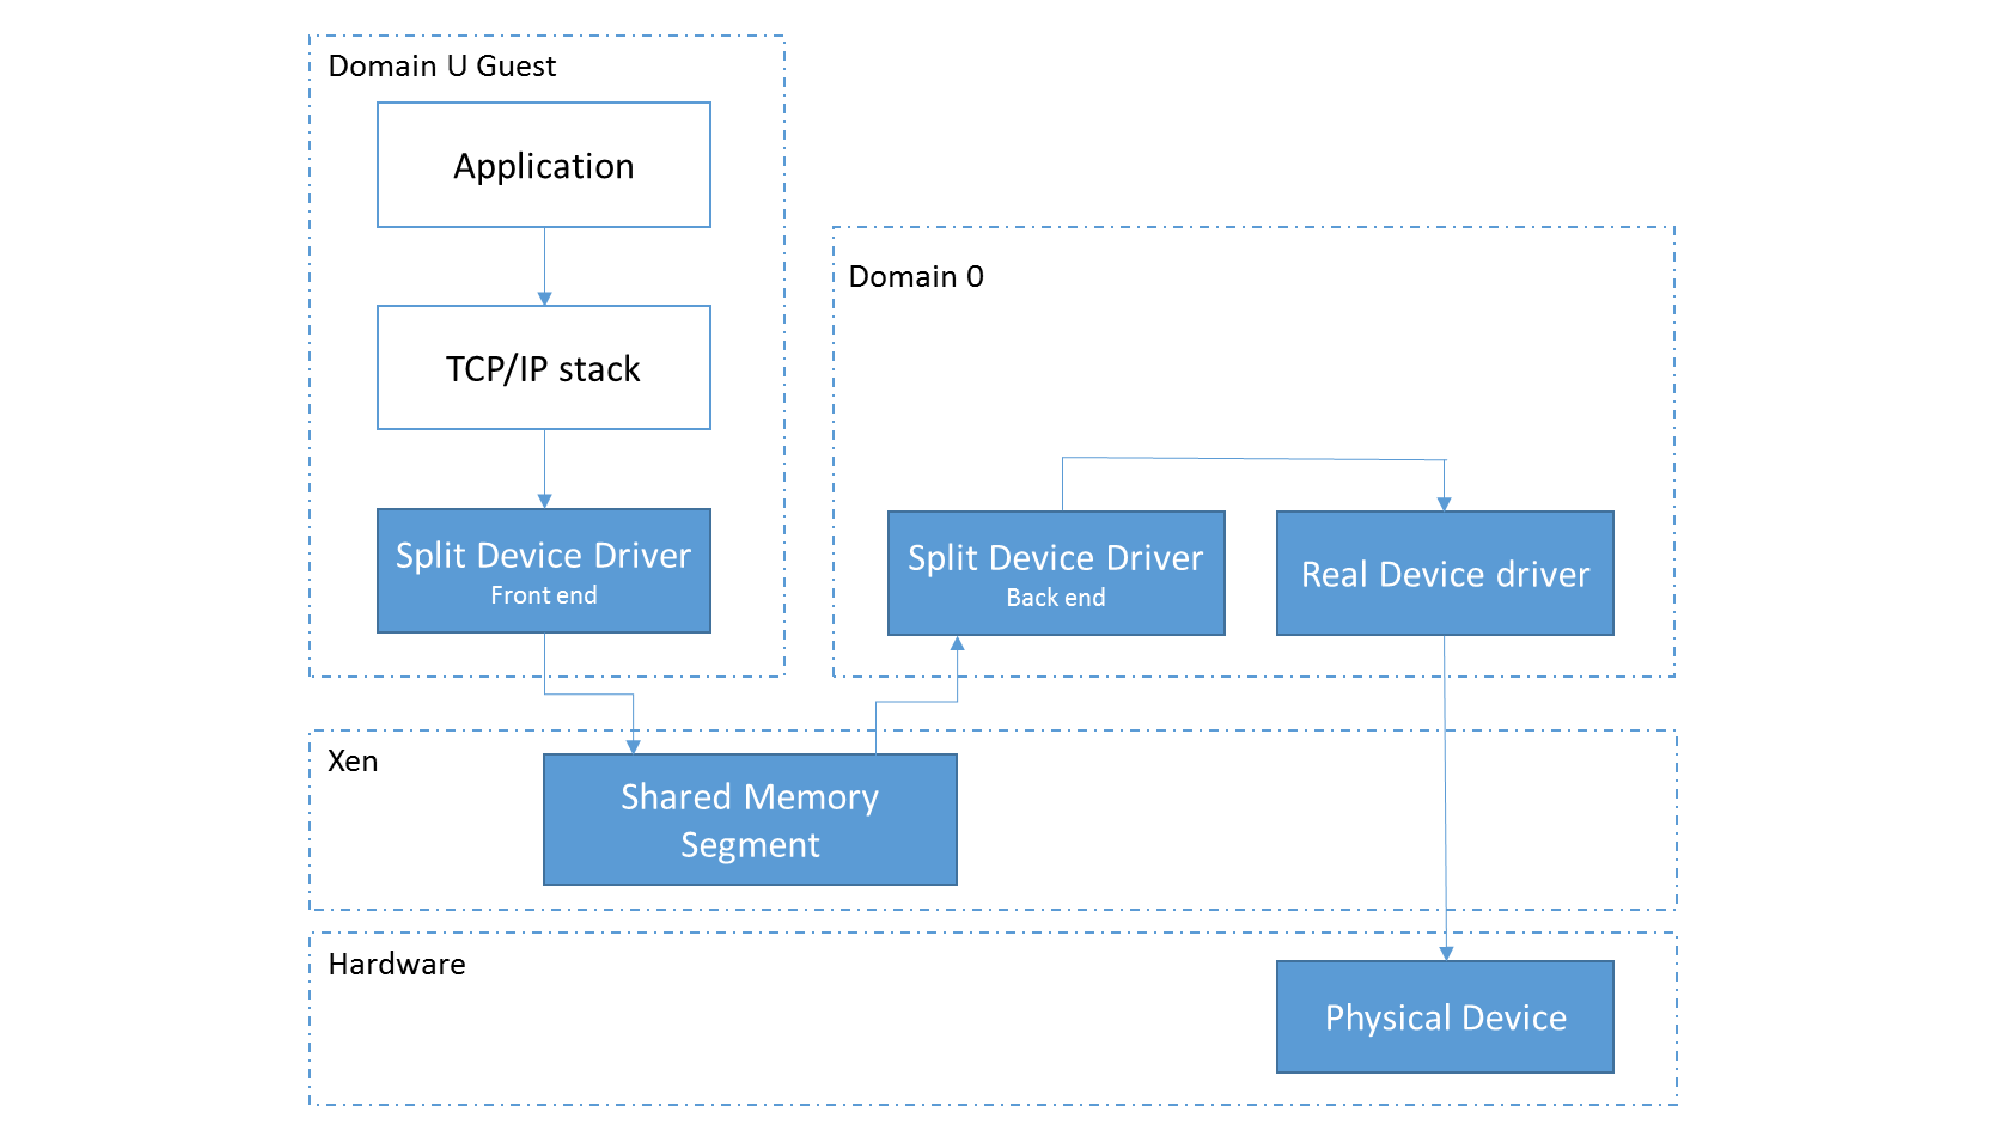
\includegraphics[scale=.50]{xen-split-tcp.pdf}
\caption{Split device driver model}
\label{fig:xen-split}
\end{figure}
Xen has a frontend driver in a domain U guest and a backend driver in the domain 0. The frontend and the backend driver transfer data between domains over a channel that is provided by the Xen VMM. Within the driver domain, the backend driver is used to demultiplex incoming data to the device and to multiplex outgoing data between the device and the guest domain~\cite{driverdomain}.
\\[3mm]
In the isolated driver domain system, user applications and a kernel are executed in a guest domain, and a device driver is executed in a driver domain. As a result, a device driver is isolated from the Linux kernel, making it impossible for the device driver to corrupt kernel data structures in the virtual machine running user applications. 
\\[3mm]
Despite advances in virtualization technology, the overhead of communication between guest and driver domains significantly affects the performance of applications~\cite{barham2003xen, Sugerman:2001:VID:647055.715774, Menon:2006:ONV:1267359.1267361}. Isolated driver domains follow an interrupt based approach for sending notifications~\cite{barham2003xen}. The frontend and backend notify each other of the receipt of a service request and corresponding responses by sending an interrupt. The Xen hypervisor needs to schedule the other domain to deliver the interrupt, which may require a context switch~\cite{barham2003xen}. Such context switches can cause system overhead~\cite{Li:2007:QCC:1281700.1281702, Mogul:1991:ECS:106973.106982}.

\section {Proposed Solution}
In this thesis, we propose and evaluate an optimization for improving the performance of the communication between guest and driver domains. We propose a solution in which a thread in the backend driver spins for some amount of time, checking for incoming service requests, and the frontend driver spins for some amount of time, checking for the responses. 
\\[3mm]
In uniprocessor and multiprocessor environment, a context switch takes a significant amount of time. In a multi-processor environment, it is more efficient for each process to keep its own CPU and spin while waiting for a resource~\cite{Bovet:2005:ULK:1077084}. Since our solution follows a spinning based approach, it performs better than the interrupt based approach used in the original implementation.
\\[3mm]
The source code of the isolated driver domain is not available in the open source Xen hypervisor code. In this thesis, we re-implement Xen's isolated driver domains, we refer to our implementation as Isolated Device Driver (IDDR). We then implement our spinning based optimization within IDDR.
\\[3mm]
The performance of the system is evaluated for multiple block device types, including ramdisks, loop devices, and SATA disks. A block device is formatted with a ext2 file system and the IDDR system is evaluated by measuring the performance of the system with SysBench benchmark. The integrity of the system is checked by executing reads and writes on a block device, with and without read ahead, file system tests on the variety of block devices. Our evaluation shows that the performance of the system can be improved by avoiding the context switches in the communication channel. The IDDR system trades off CPU cycles for the better performance. It uses CPU cycles spinning while waiting for requests and responses. Otherwise, these CPU cycles would have been used by an application.

\section{Core Contributions}
The core contributions of this project are listed below: 
\begin{enumerate}
\item Re-implementation of Xen's isolated driver domain - Isolated Device Driver (IDDR).
\item Improvement in the performance of the IDDR by implementing the spinning based communication channel instead of the interrupt based communication channel. 
\item A performance comparison of the spinning based IDDR and interrupt based IDDR.
\end{enumerate}
\section {Organization}
This section provides the organization and roadmap of the thesis.
\begin{enumerate}
\item Chapter 2 provides background on Processes, Threads, Memory Protection, Virtualization, Hypervisor and Inter-domain Communication.
\item Chapter 3 provides an introduction to design of the system to isolate device driver. 
\item Chapter 4 discusses the detailed design and implementation of IDDR. 
\item Chapter 5 evaluates the performance of IDDR.
\item Chapter 6 reviews related work in the area of kernel fault tolerance.
\item Chapter 7 concludes the thesis and lists possible topics where this work can be extended.
\end{enumerate}
\pagebreak
\ifbool{toShowBibliography}{\bibliography{references}}{}

\chapter{Background}  
\markright{Sushrut Shirole \hfill Chapter 2. Background \hfill}

This section provides background on operating system terminology such
as processes, threads, memory protection, virtualization and hypervisors.

\section{Processes and Threads}
\paragraph{Process:} A process can be viewed both as a program in execution
and as an abstraction of a processor. Each process has its own address
space~\cite{Galvin}.

\paragraph{Threads:} A process has either a single or multiple threads
sharing its address space. Each thread represents a separate flow of
control~\cite{Galvin}.

A thread is also called a light-weight process. The implementation of
threads and processes differs between operating systems. A process's 
threads share resources such as code and data segments, whereas 
different processes do not share such resources.
\begin{figure}[!ht]
    \centering
    \begin{subfigure}[b]{0.45\textwidth}
	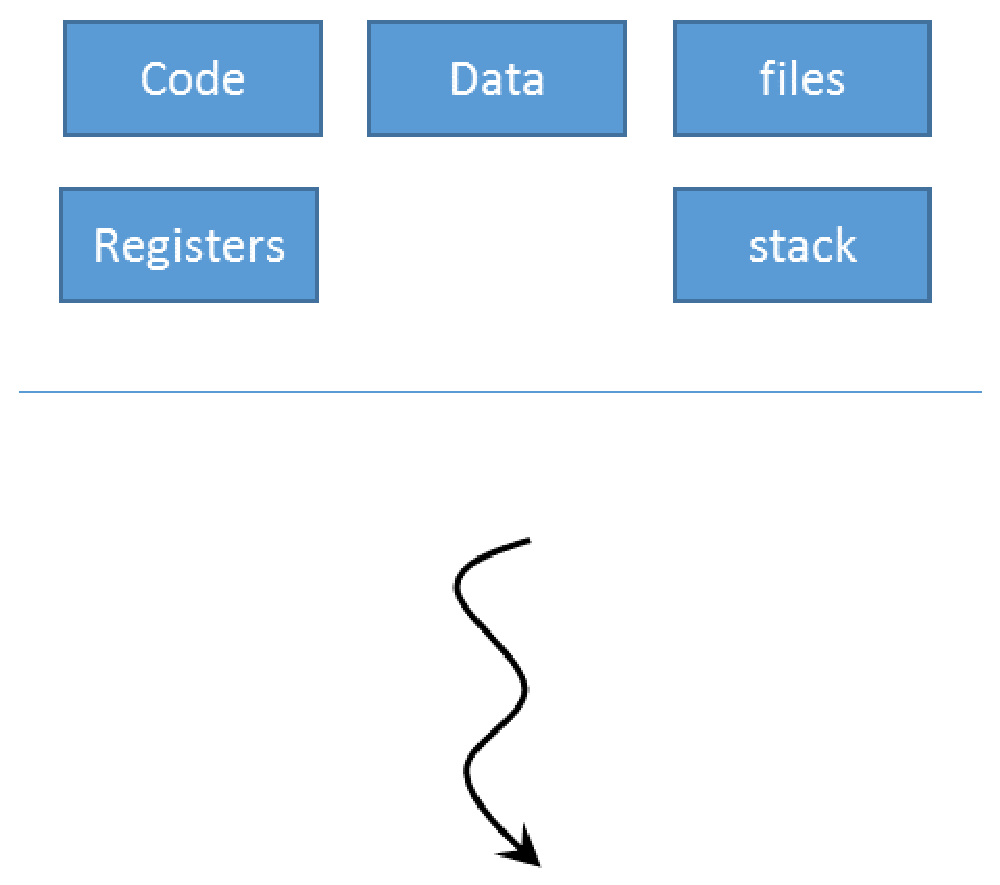
\includegraphics[scale=.25]{thread1}
	\caption{Single-threaded process}
	\label{fig:thread1}
    \end{subfigure}
	\hfill
    \begin{subfigure}[b]{0.45\textwidth}
	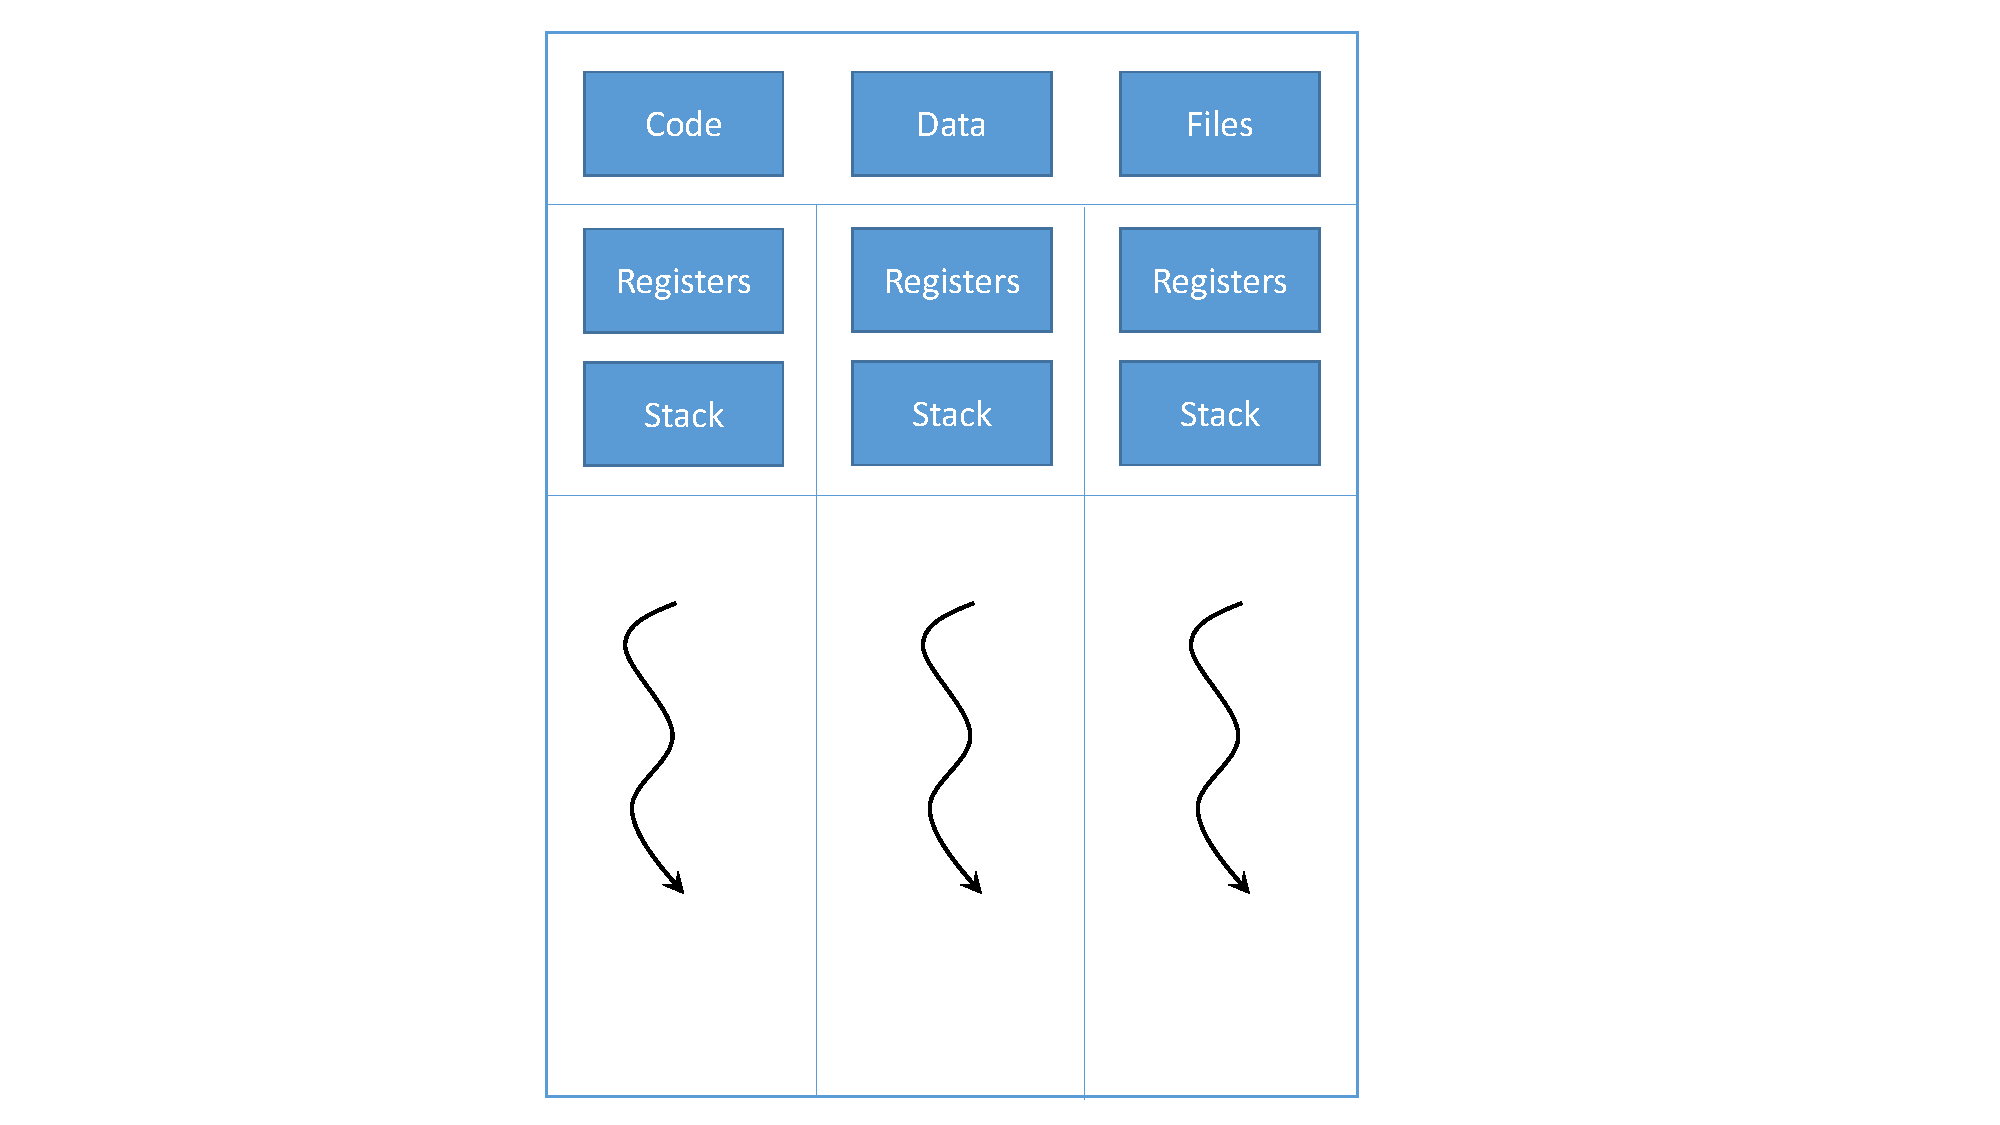
\includegraphics[scale=.25]{thread2}
	\caption{Multithreaded process}
	\label{fig:thread2}
    \end{subfigure}
    \caption{Thread}\label{fig:threads}
\end{figure}

\section{Context Switch}
Multiple threads typically employ time division multiplexing when sharing
a single processor.  In time division multiplexing, the processor switches
between executing threads, interleaving their execution. The process of 
switching between threads is called a context switch. Continuous context switching
creates the impression for the user that threads and processes are
running concurrently. On multiprocessor systems, threads can also run
simultaneously on multiple processors, each of which may perform time
division multiplexing.

During a context switch the state of a thread is saved so that its
execution can be resumed from the same point at a later time. The
composition of the saved state is determined by the processor and the operating system
~\cite{Galvin}. The costs of context switches can be divided into direct and
indirect costs. The direct cost is the time required to save and restore
processor registers, execute the scheduler code, flush TLB entries and
to flush the processor pipeline. Indirect costs include subsequent cache miss 
penalties that are due to processor 
pollution~\cite{Soares+:osdi10, Li:2007:QCC:1281700.1281702}.

\section{Spinlocks}
In uniprocessor and multiprocessor environments, a context switch takes a
significant amount of time.  In a multi-processor environment, it may be more
efficient for each process to keep its own CPU and spin while waiting
for a resource.

A spinlock is a locking mechanism designed to work in a multiprocessor
environment. A spinlock causes a thread that is trying to acquire lock
to spin if the lock is not immediately available~\cite{Bovet:2005:ULK:1077084}.

\textbf{Adaptive Spinning} is a spinlock optimization technique. 
After unsuccessfully spinning for a set threshold amount of time, a thread
will block as for regular locks.
In the adaptive spinning technique, the spinning threshold is determined by
an algorithm based on the rate of successes and failures of recent spinning
attempts to acquire the lock.  Adaptive spinning helps threads to avoid
spinning in conditions where it would not be beneficial.

\section{Device Driver}
\label{sec:device driver}

A device driver is a program that provides a software interface to a
particular hardware device. It enables the operating system and other
programs to access its hardware functions. Device drivers are hardware
dependent and operating system specific.  A driver issues commands to 
a device in response to system calls requested by user programs.
After executing these commands,
the device sends data back to the driver. The driver informs the caller by 
invoking callback routines after receiving the data. The Linux
kernel distinguishes between three device types: character devices,
block devices, and network interfaces.

\begin{figure}[!ht]
\centering
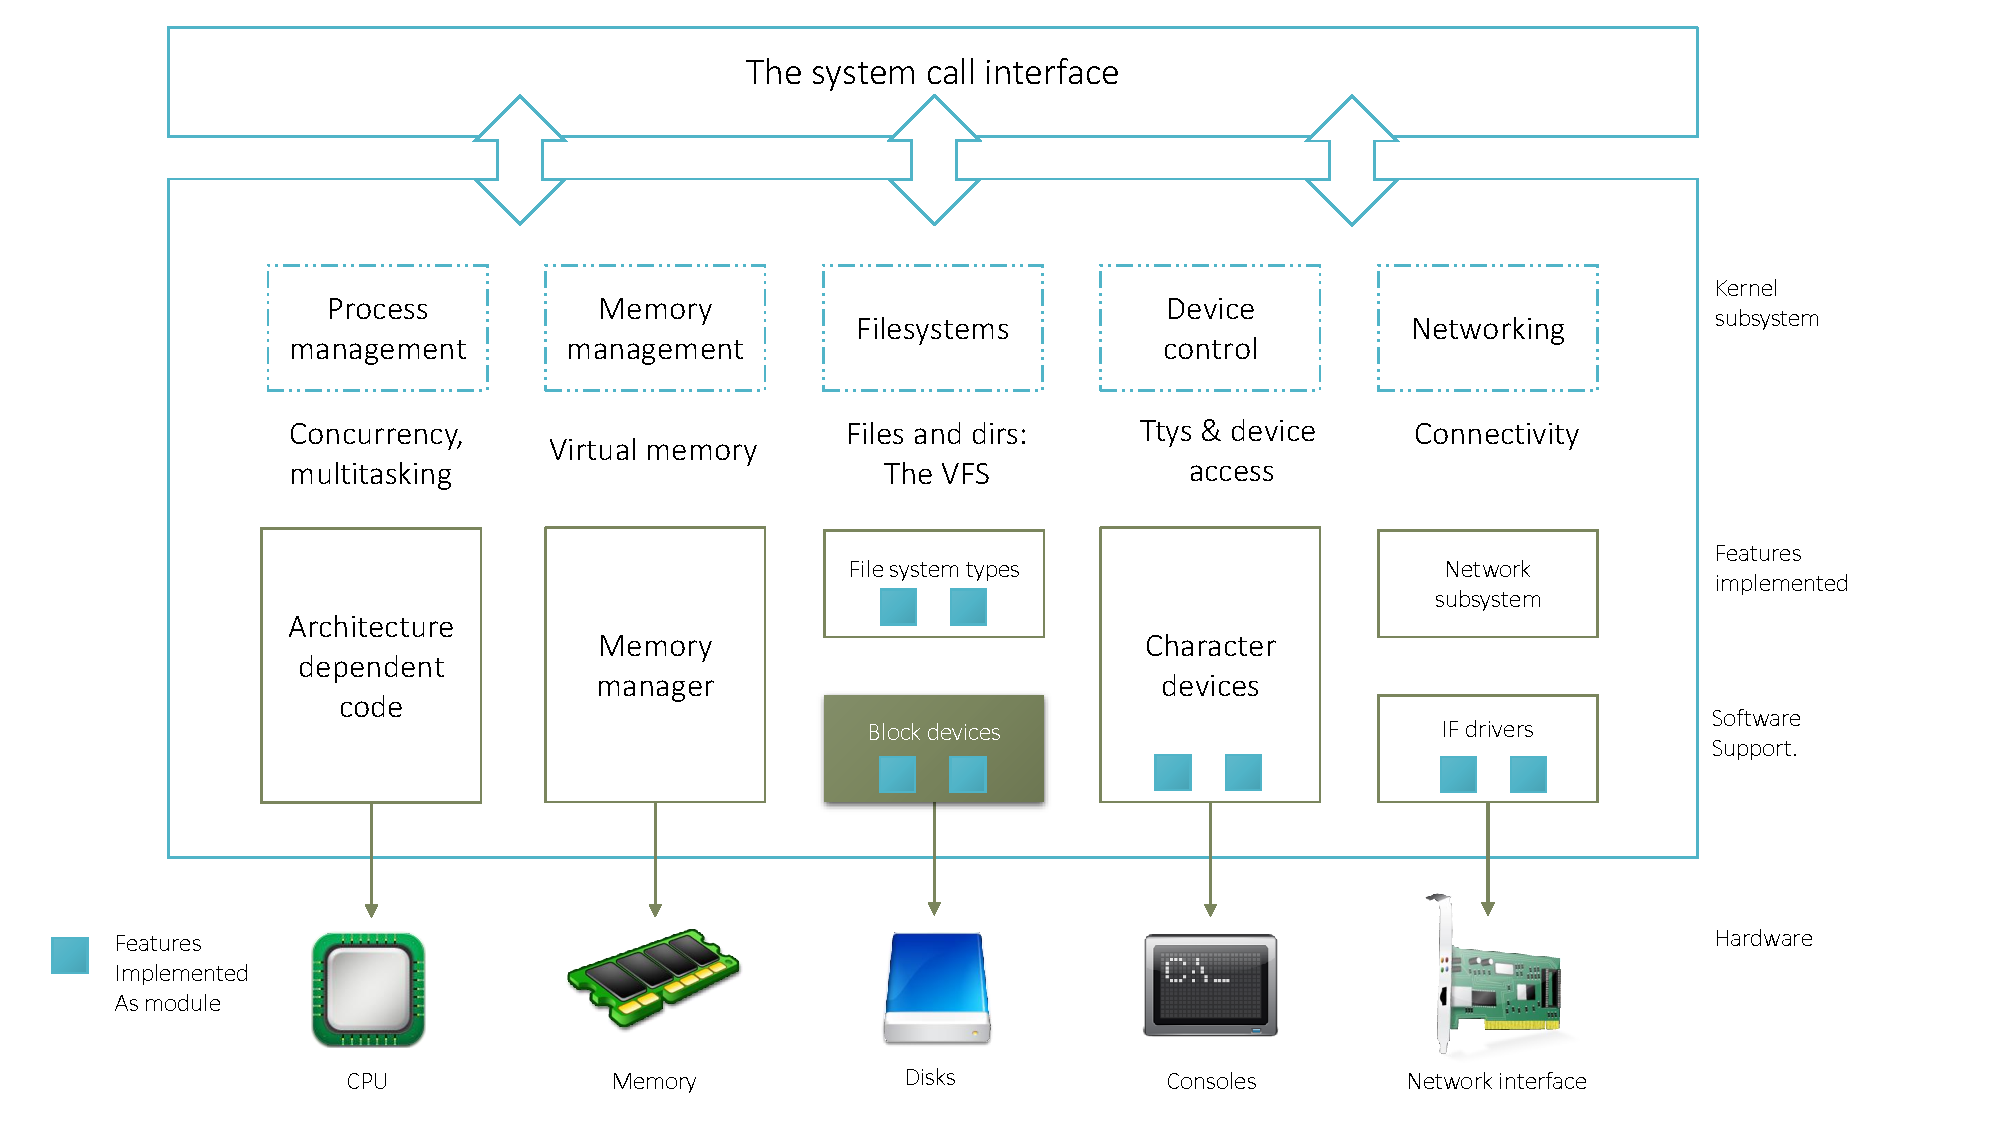
\includegraphics[scale=.5 ]{kernel}
\caption{Split view of a kernel}
\label{fig:kernel}
\end{figure}

\paragraph{Character devices:} A character device can be accessed as
a stream of bytes. A character driver usually implements at least the
open, close, read, and write functions. The text console (/dev/console)
and the serial ports (/dev/ttyS0) are examples of character devices.

\paragraph{Network Interfaces:} A network interface is a device that
is able to exchange data with other hosts. Usually, a network interface
is a hardware device, but it can be a software device such as the loopback
interface.

\paragraph{Block Devices:} Unlike character devices, block devices
are accessed as blocks of data. Whereas most Unix implementations
support only I/O operations that involve entire blocks,
Linux also allows applications to read and write individual bytes within
a block. As a result, in Linux, block and char devices
differ only in the way data is managed internally by the kernel. 
Examples of block devices are disks and CDs~\cite{Corbet:2005:LDD:1209083}.

\subsection*{Block Device Driver}
\subsubsection*{Request processing in a block device driver}

\label{subsec:request queue}
A block device driver maintains a request queue to store read and write
requests. In order to initialize a request queue, a spinlock and a
request function pointer is required.  The request function forms
the central part of the block device driver. Requests are added to
the request queue when a request is made by higher level code in the
Linux kernel, such as a file system. A block device driver's
request function is called after receiving a new request. The request function
must remove all requests from the head of the request queue and send
them to the block device for execution. The Linux kernel acquires a
spinlock before calling the request function and releases it after
returning. As a result, a request function runs in a mutually 
exclusive context~\cite{Corbet:2005:LDD:1209083}.

A request is a linked list of \texttt{struct bio} objects. The \texttt{bio} 
structure contains all the information required to execute a read or write
operation on a block device. The block I/O code receives the bio
structure from the higher level code in the Linux kernel. The
block I/O code may add the received bio structure to an existing
request~\cite{Corbet:2005:LDD:1209083}, if any, or it must create
a new request.

Each bio structure in a request describes the low level block I/O
request. If possible, the Linux kernel merges several independent
requests to form one block I/O request. Usually the kernel combines
multiple requests if they require access to adjacent sectors on
the disk. However, it never combines read and write requests.

\section{Memory Protection}

The memory protection mechanism of a computer system controls
access to resources. The goal of memory protection is to prevent
malicious misuse of the system by users or programs. Memory
protection also ensures that a resource is used in accordance
with the system policies. In addition, it also helps to
ensure that errant programs cause minimal damage~\cite{Galvin,
Graham:1971:PPP:1478873.1478928}. Subsection~\ref{subsec:user level}
and subsection~\ref{subsec:kernel level} explain the policies implemented
at kernel level and user level.

\subsection{User Level}
\label{subsec:user level}
%
% ............. CONTINUE HERE
%

Typically in a monolithic kernel, the lowest \texttt{X Gb} of memory is
reserved for user processes. The upper \texttt{Virtual Memory size - X Gb}
is reserved for the kernel. The kernel puts its private data structures
in the upper memory and always accesses them at the same virtual address.

\begin{figure}[!ht]
\centering
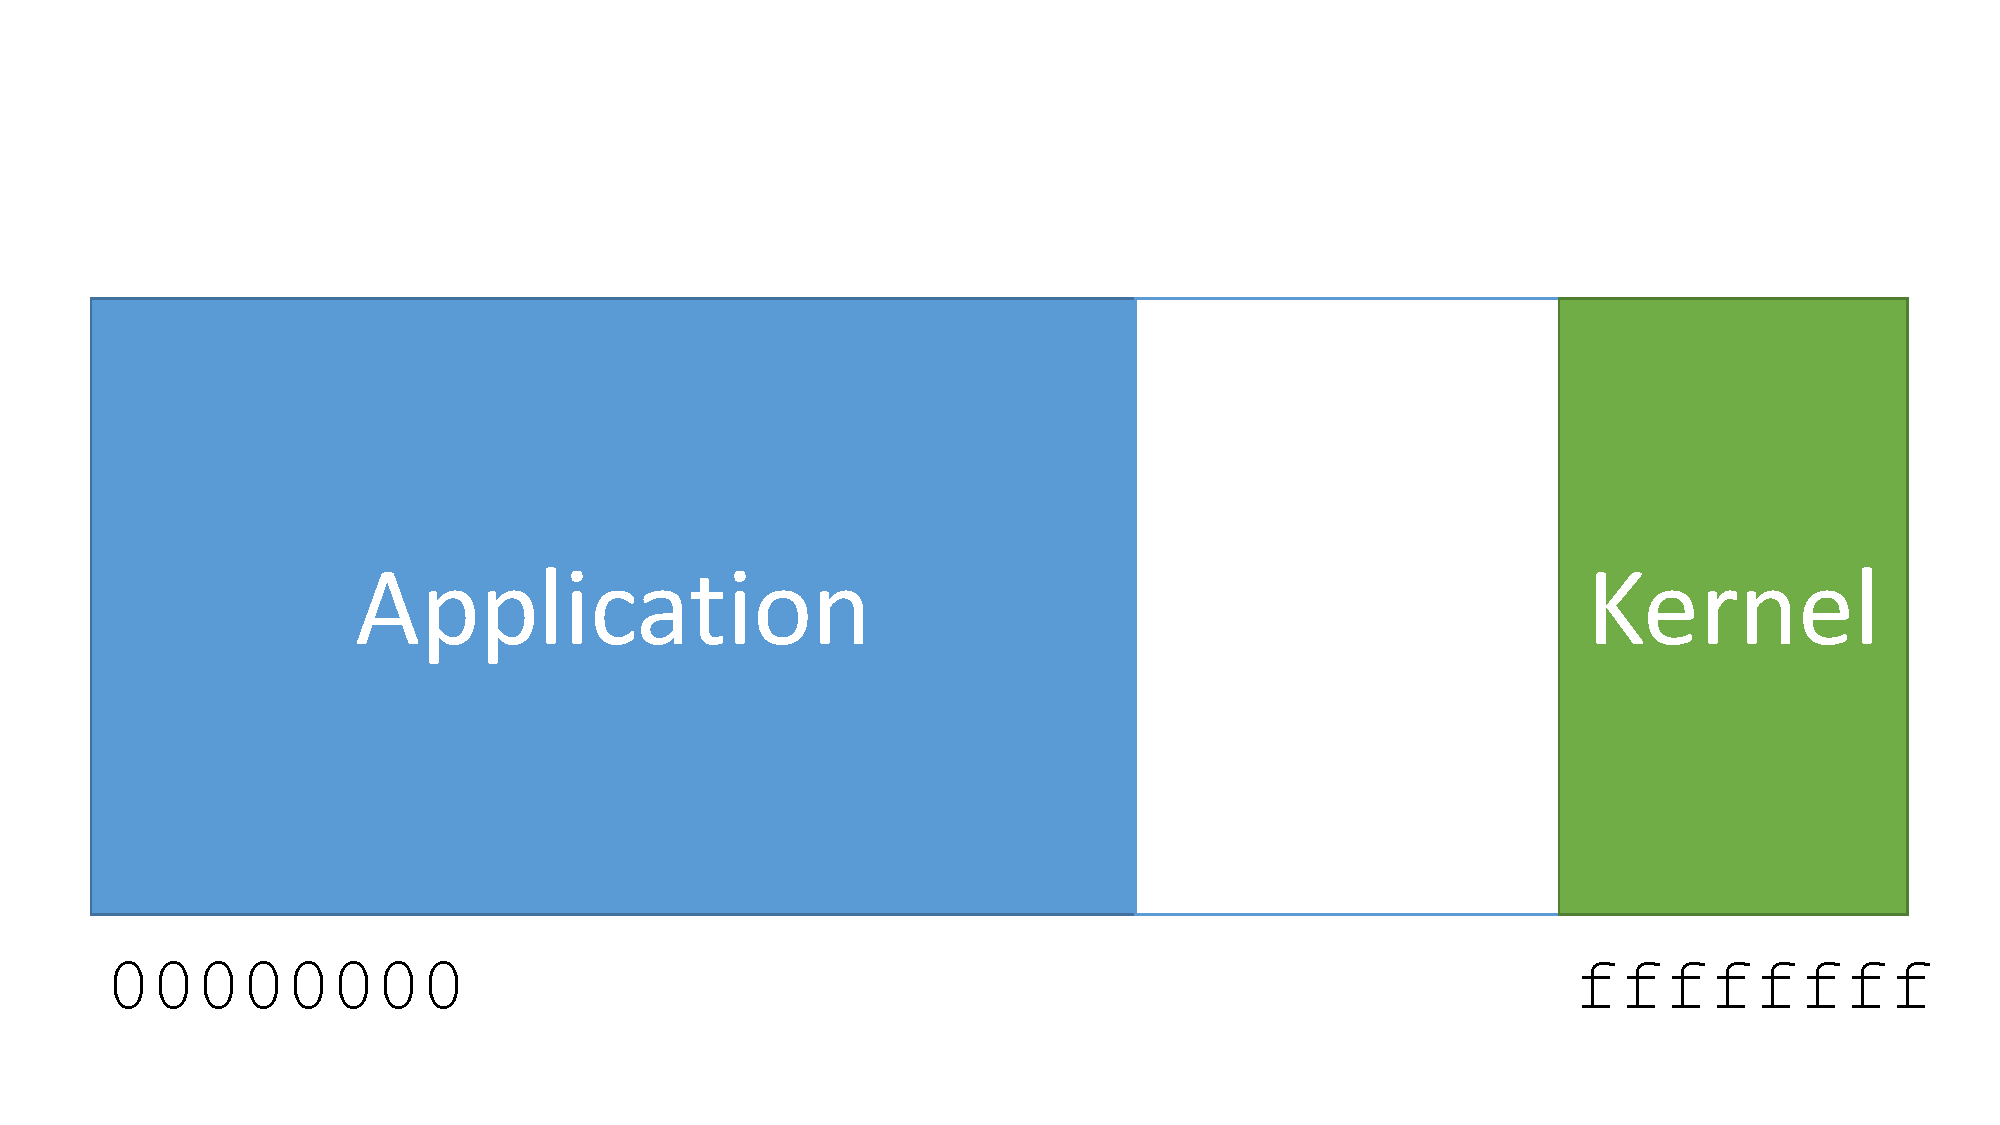
\includegraphics[scale=.25 ]{memory_map}
\caption{Physical memory}
\label{fig:memmap}
\end{figure}

At the user space, each application runs as a separate process. Each
process is associated with an address space and believes that it owns the
entire memory, starting with the virtual address 0. However, a translation
table translates every memory reference by these processes from virtual
to physical addresses. The translation table maintains \texttt{$<$base,
bound$>$} entries. If a process tries to access virtual address that
is outside the \texttt{base + bound} address, then an error is reported
by the operating system, otherwise the physical address \texttt{base +
virtual address} is returned. This allows multiple processes to be run in
the memory with protection. Since address translation provides protection,
a process cannot access addresses outside its address space.

Consider the example shown in Figure~\ref{fig:User space}.
\begin{enumerate}
\item This system is running 3 different user processes
\item One of the processes encounters a bug and tries to access a memory address outside its address space
\item Access to the address is restricted by the memory protection mechanism
\begin{figure}[!ht]
    \centering
    \begin{subfigure}[b]{0.49\textwidth}
	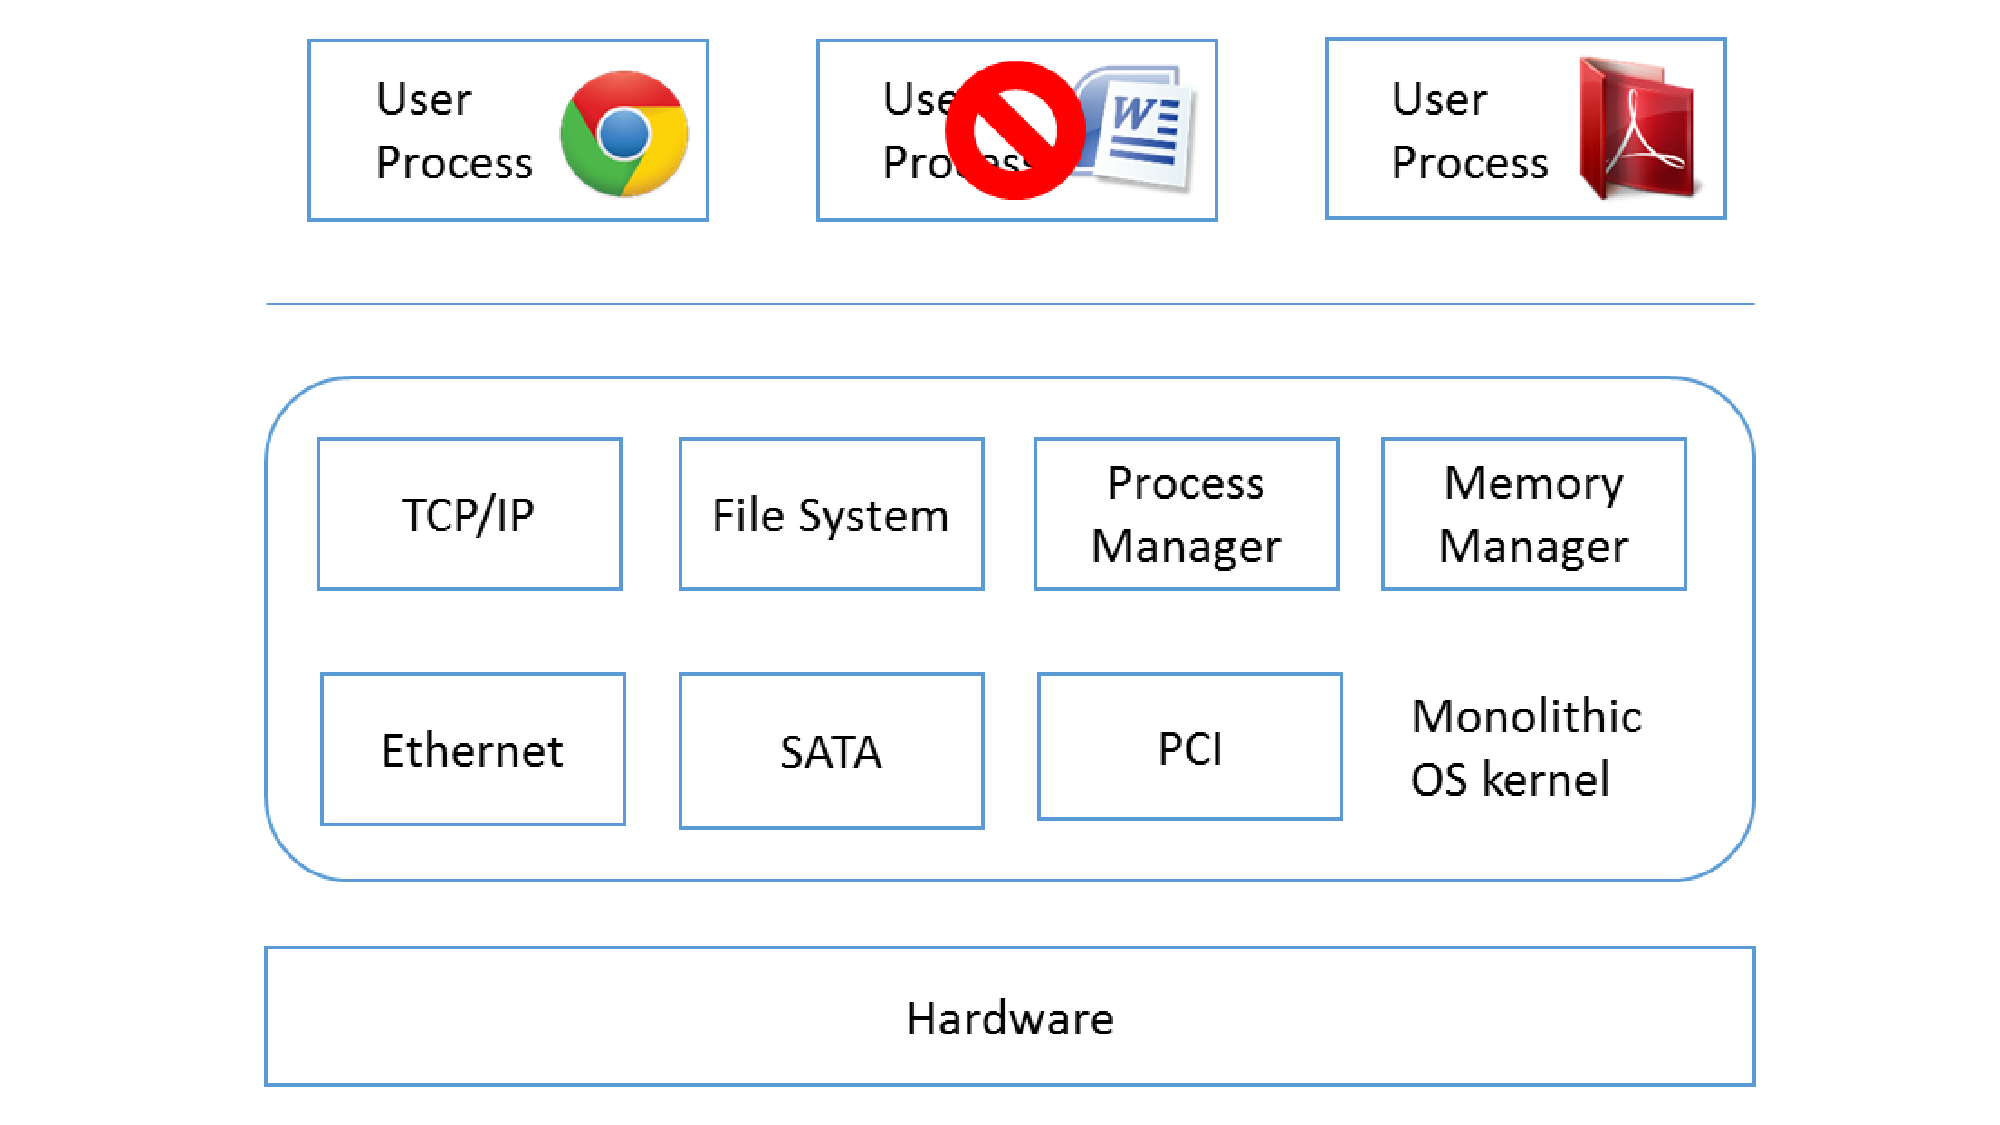
\includegraphics[scale=.25]{user-space-1}
	\caption{A process encounters a bug}
    \end{subfigure}
	\hfill
    \begin{subfigure}[b]{0.49\textwidth}
	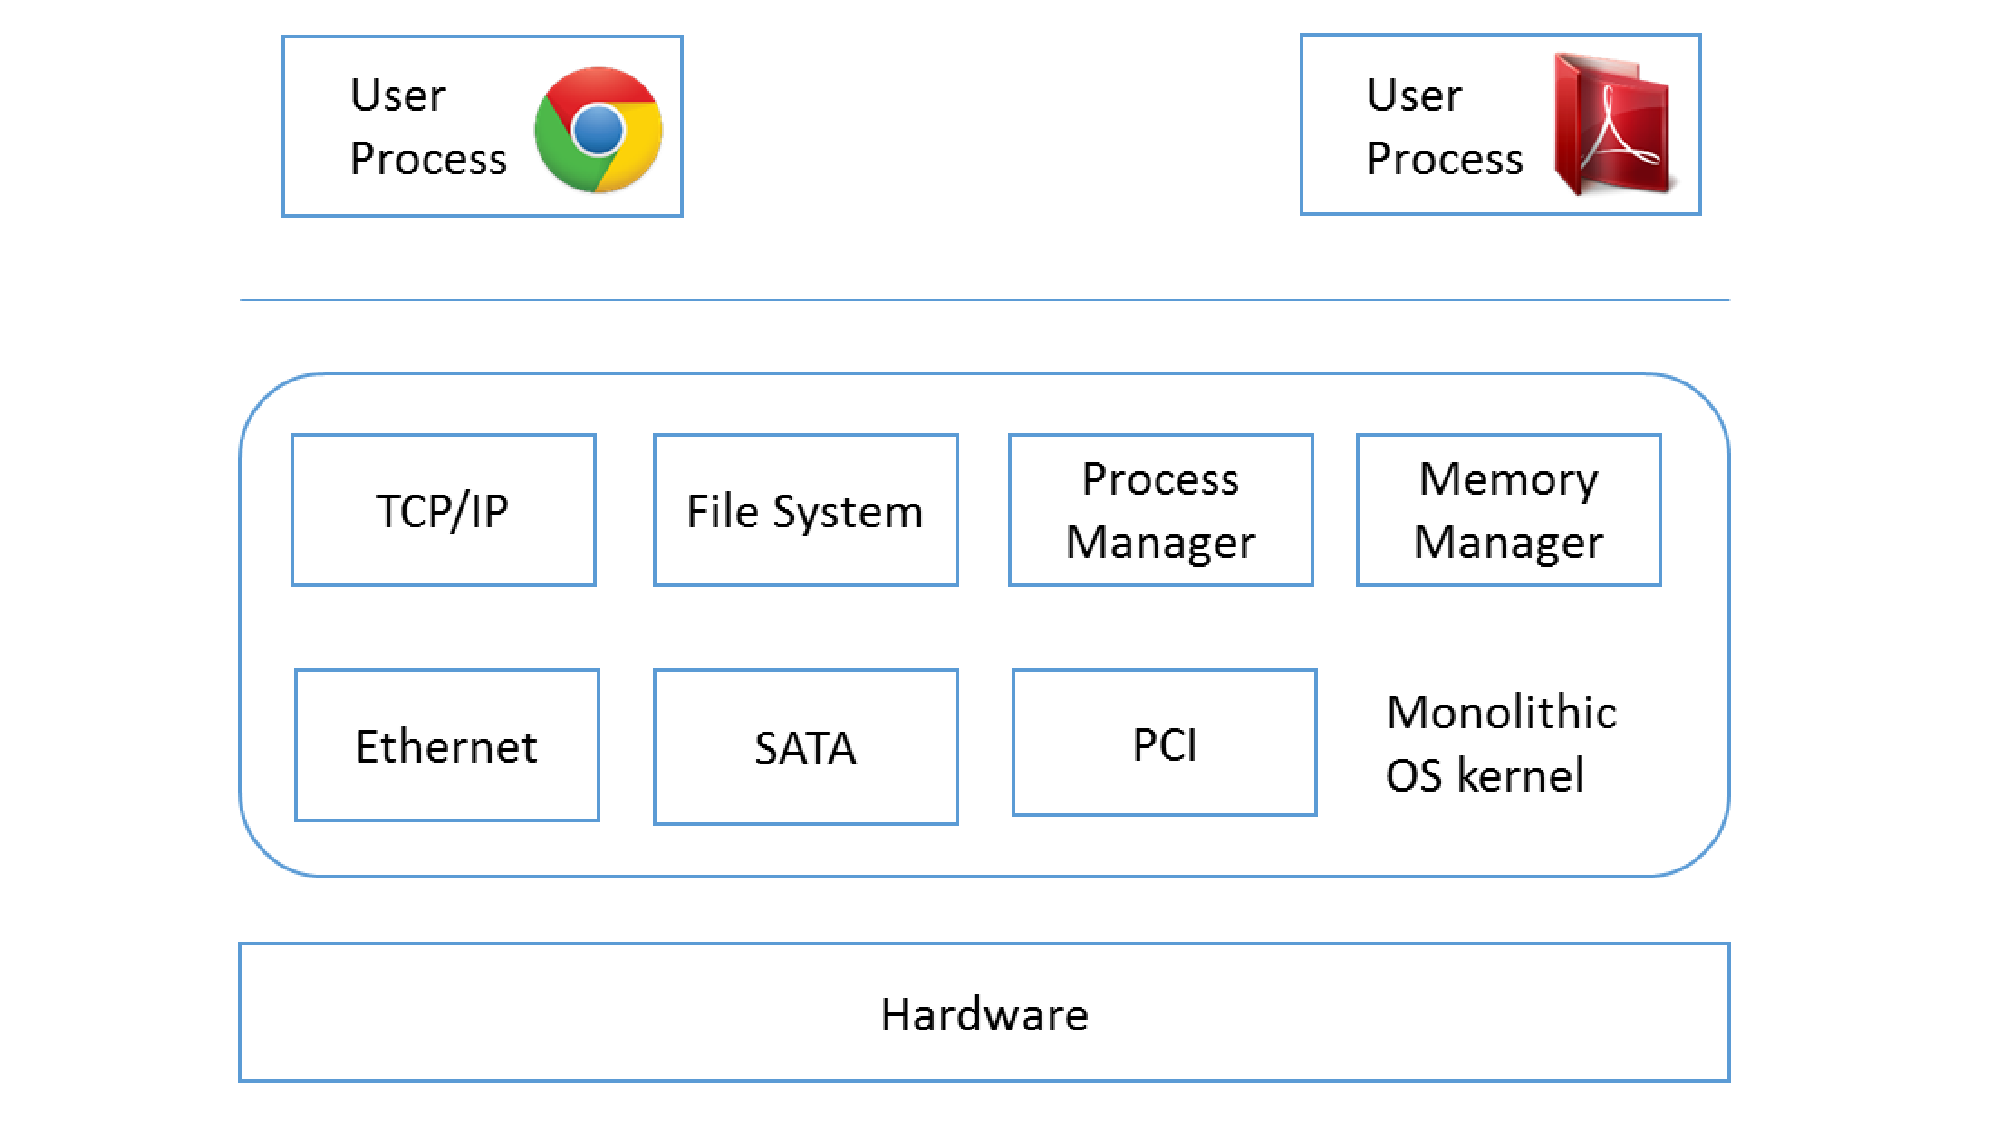
\includegraphics[scale=.25]{user-space-2}
	\caption{Other user processes are not affected}
    \end{subfigure}
    \caption{User level memory protection}\label{fig:User space}
\end{figure}
\end{enumerate}

\subsection{Kernel Level}
\label{subsec:kernel level}
This sections explains how memory is managed at kernel level. 

In a Linux kernel, virtual memory is divided into pages and physical memory is divided into blocks called as page frames. Linux kernel uses a data structure called page table to store virtual memory to physical memory mapping information. Kernel reserves upper virtual memory for its internal use. The page table entries of this region are marked as protected so that pages are not visible or modifiable in the user mode. However, at kernel level any code running at priviledged level can access the kernel memory. Hence a kernel component can access, and potentially, corrupt any kernel data structures.

Consider the example shown in Figure~\ref{fig:Kernel space}
\begin{enumerate}
\item The system runs 3 different processes in the user space and has different kernel components running in kernel space.
\item The network driver hits a bug, and corrupts kernel data structures. The corruption might lead to a system crash.
\end{enumerate}
\begin{figure}[!ht]
    \centering
    \begin{subfigure}[b]{0.49\textwidth}
	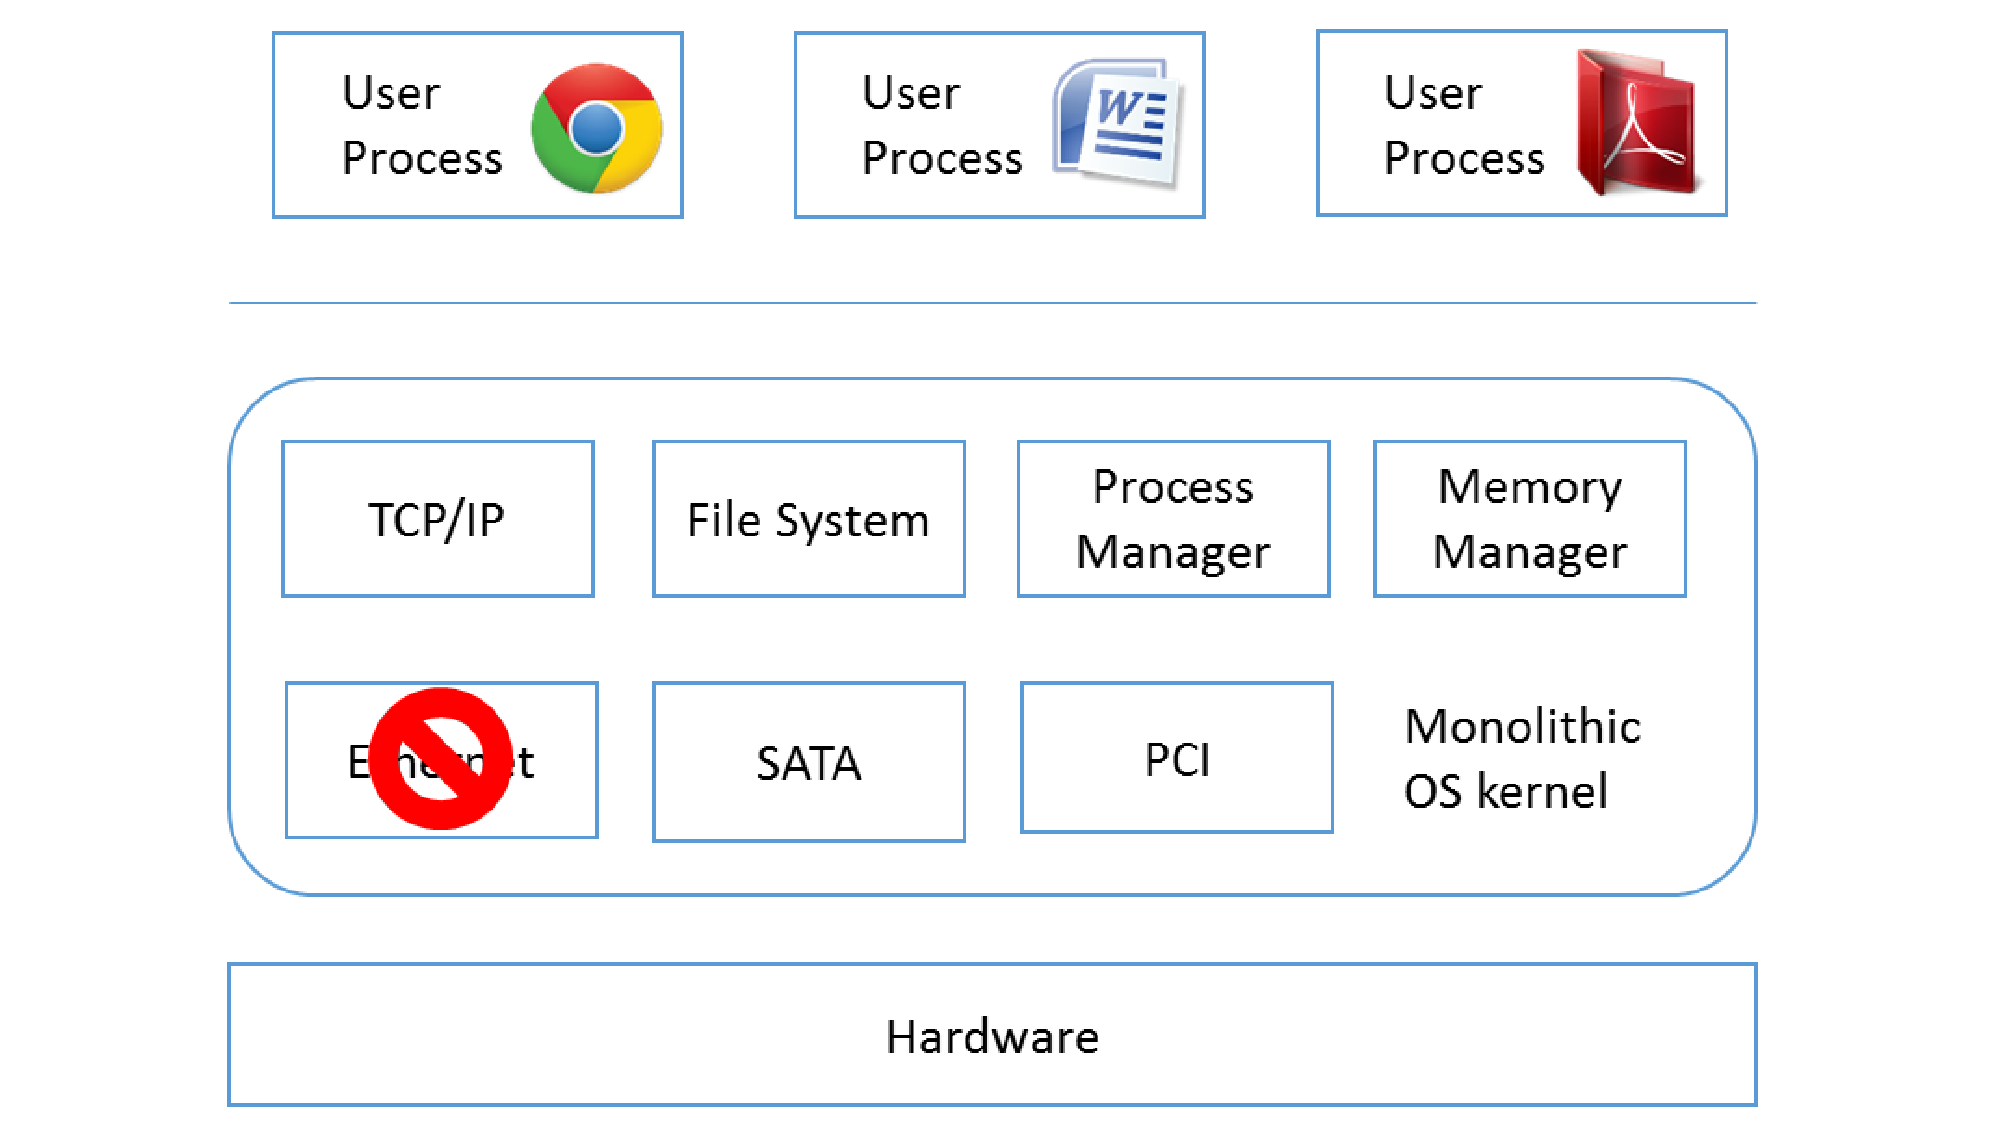
\includegraphics[scale=.25]{kernel-space-1}
	\caption{A kernel component hits a bug}
    \end{subfigure}
	\hfill
    \begin{subfigure}[b]{0.49\textwidth}
	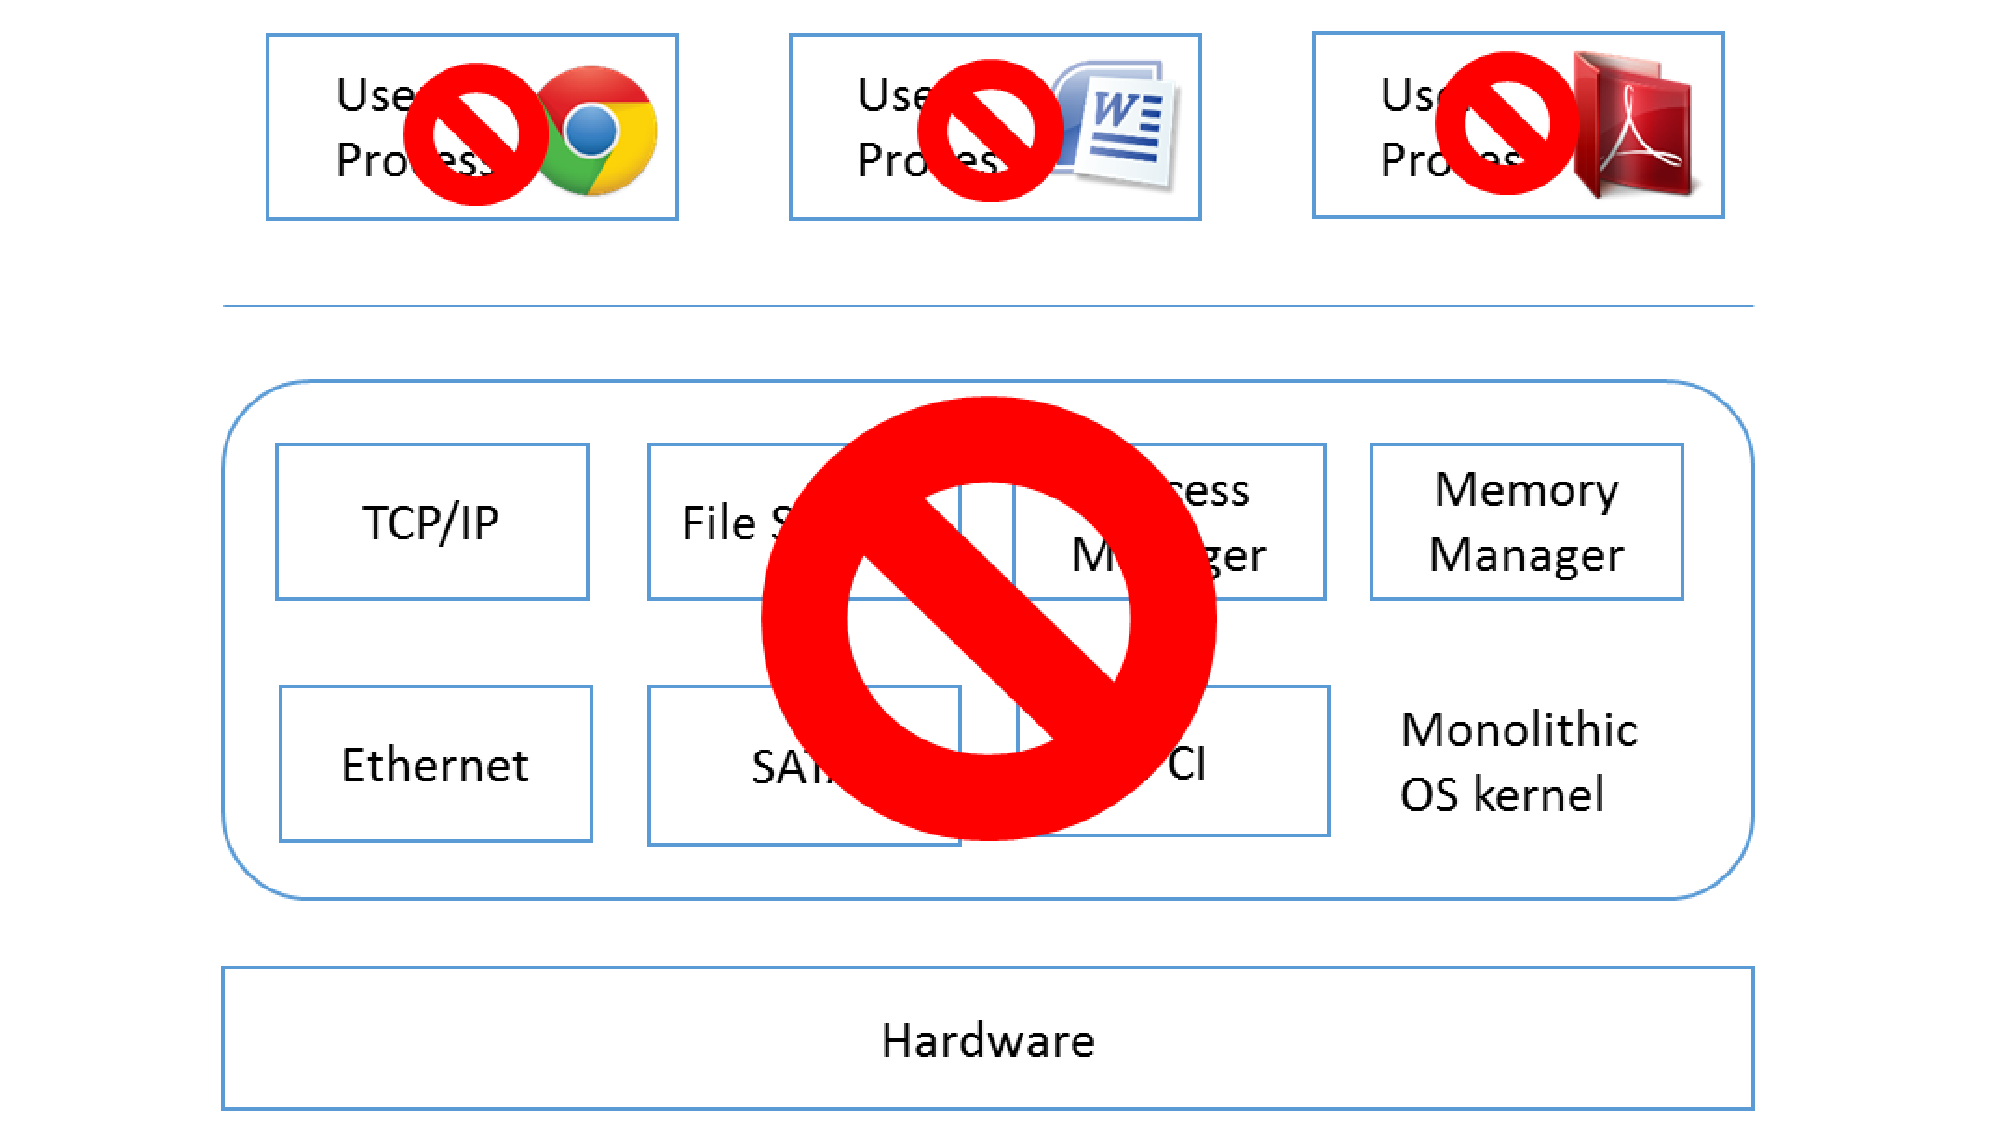
\includegraphics[scale=.25]{kernel-space-2}
	\caption{Results in a system crash}
    \end{subfigure}
    \caption{Kernel level memory protection}\label{fig:Kernel space}
\end{figure}

\section{Virtualization}

Virtualization is the act of creating an abstraction of the hardware of a single machine into several different execution environments. Such abstraction creates the illusion that each separate execution environment is running its own private machine~\cite{Galvin}. 

Virtualization provides the capability to share the underlying hardware resources and still provide an isolated environment to each operating system. Because of this isolation, any failures in an operating system can be contained. Virtualization can be implemented in many different ways, either with or without hardware support. Operating systems might require some changes in order to run in a virtualized environment~\cite{Drepper:2008:CV:1348583.1348591}. It has been shown that virtualization can be utilized to provide better security and robustness for operating systems~\cite{Fraser04safehardware, LeVasseur04UnmodifiedDriverReuse, Riley:2008:GPK:1433006.1433008}.
\begin{figure}[!ht]
    \centering
    \begin{subfigure}[b]{0.49\textwidth}
	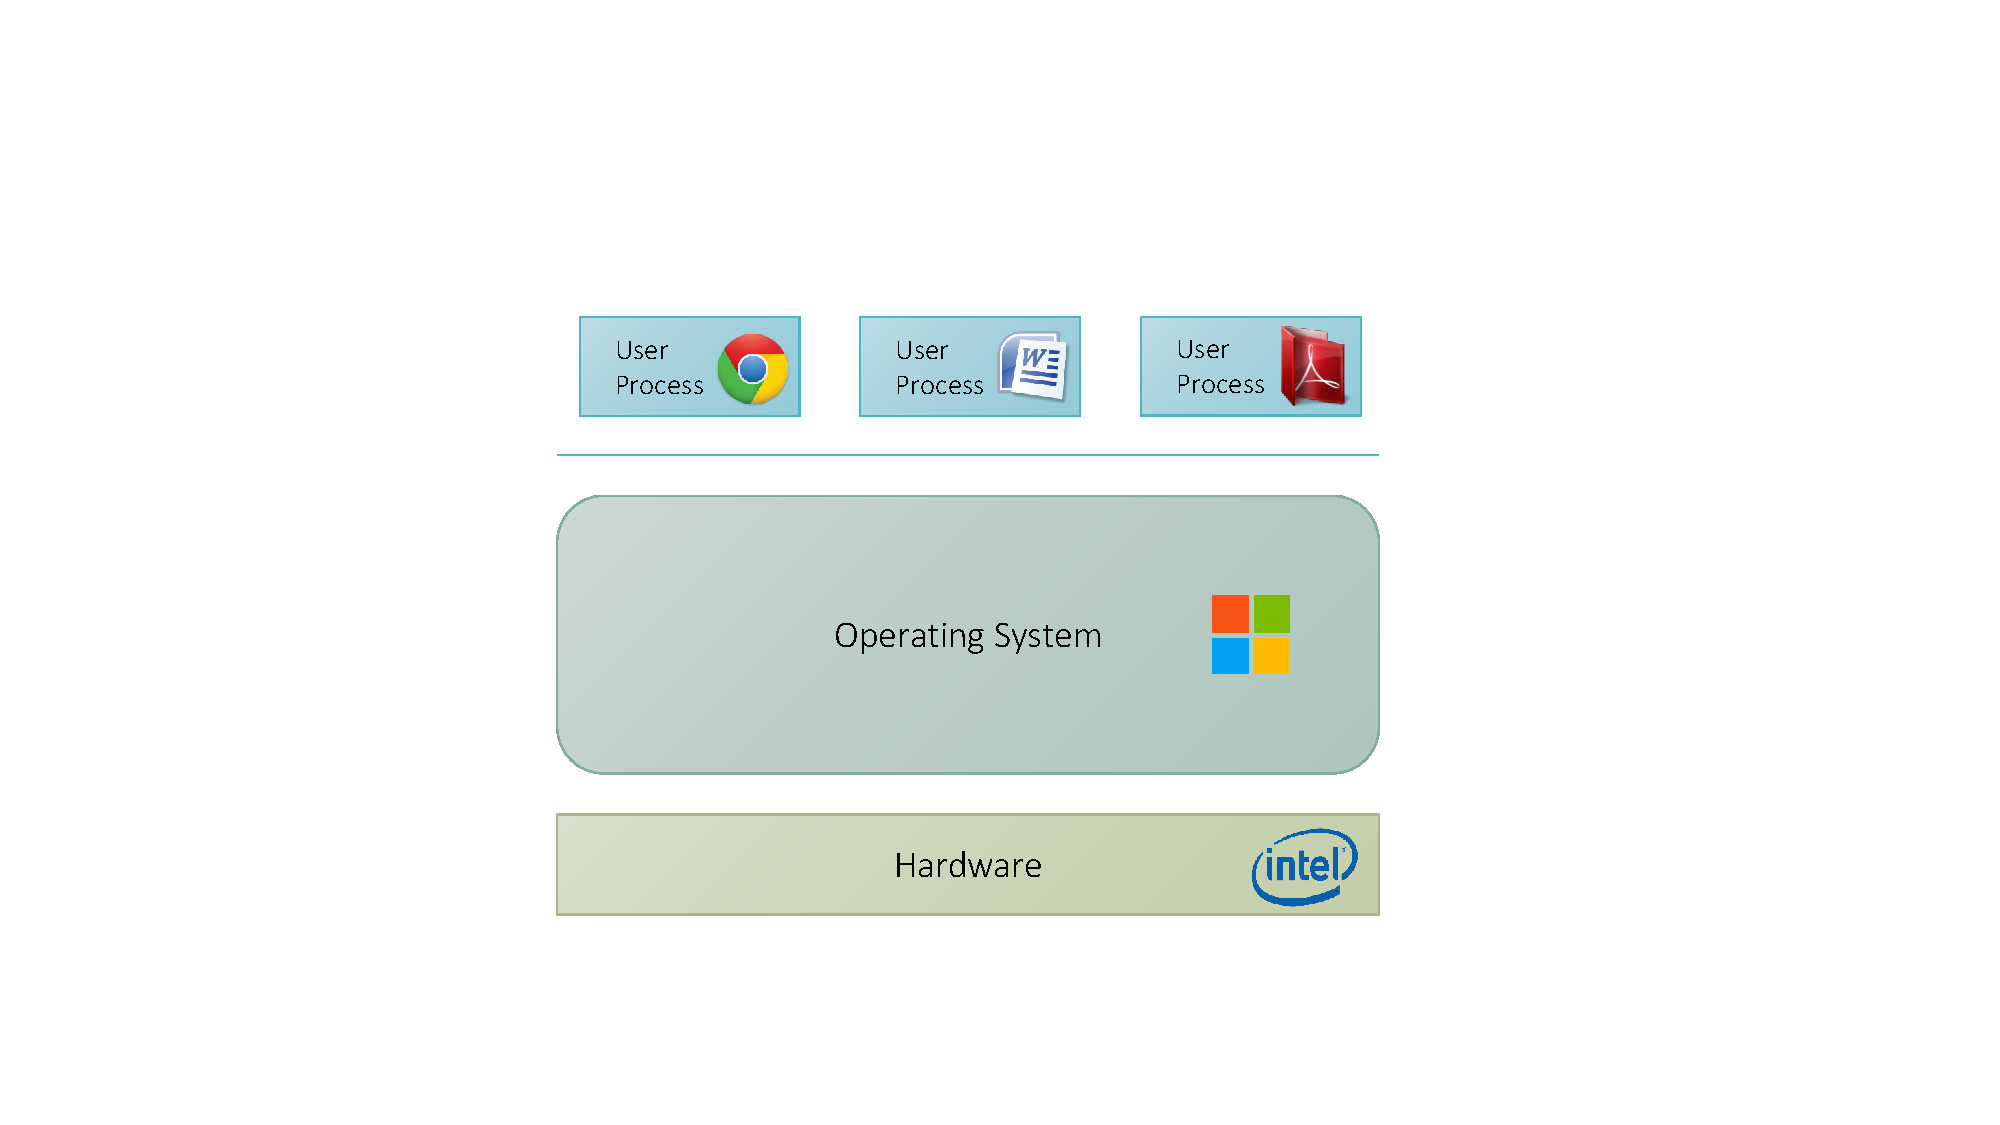
\includegraphics[scale=.25]{OS-arch}
	\caption{Operating System Architecture}
	\label{fig:OS}
    \end{subfigure}
	\hfill
    \begin{subfigure}[b]{0.49\textwidth}
	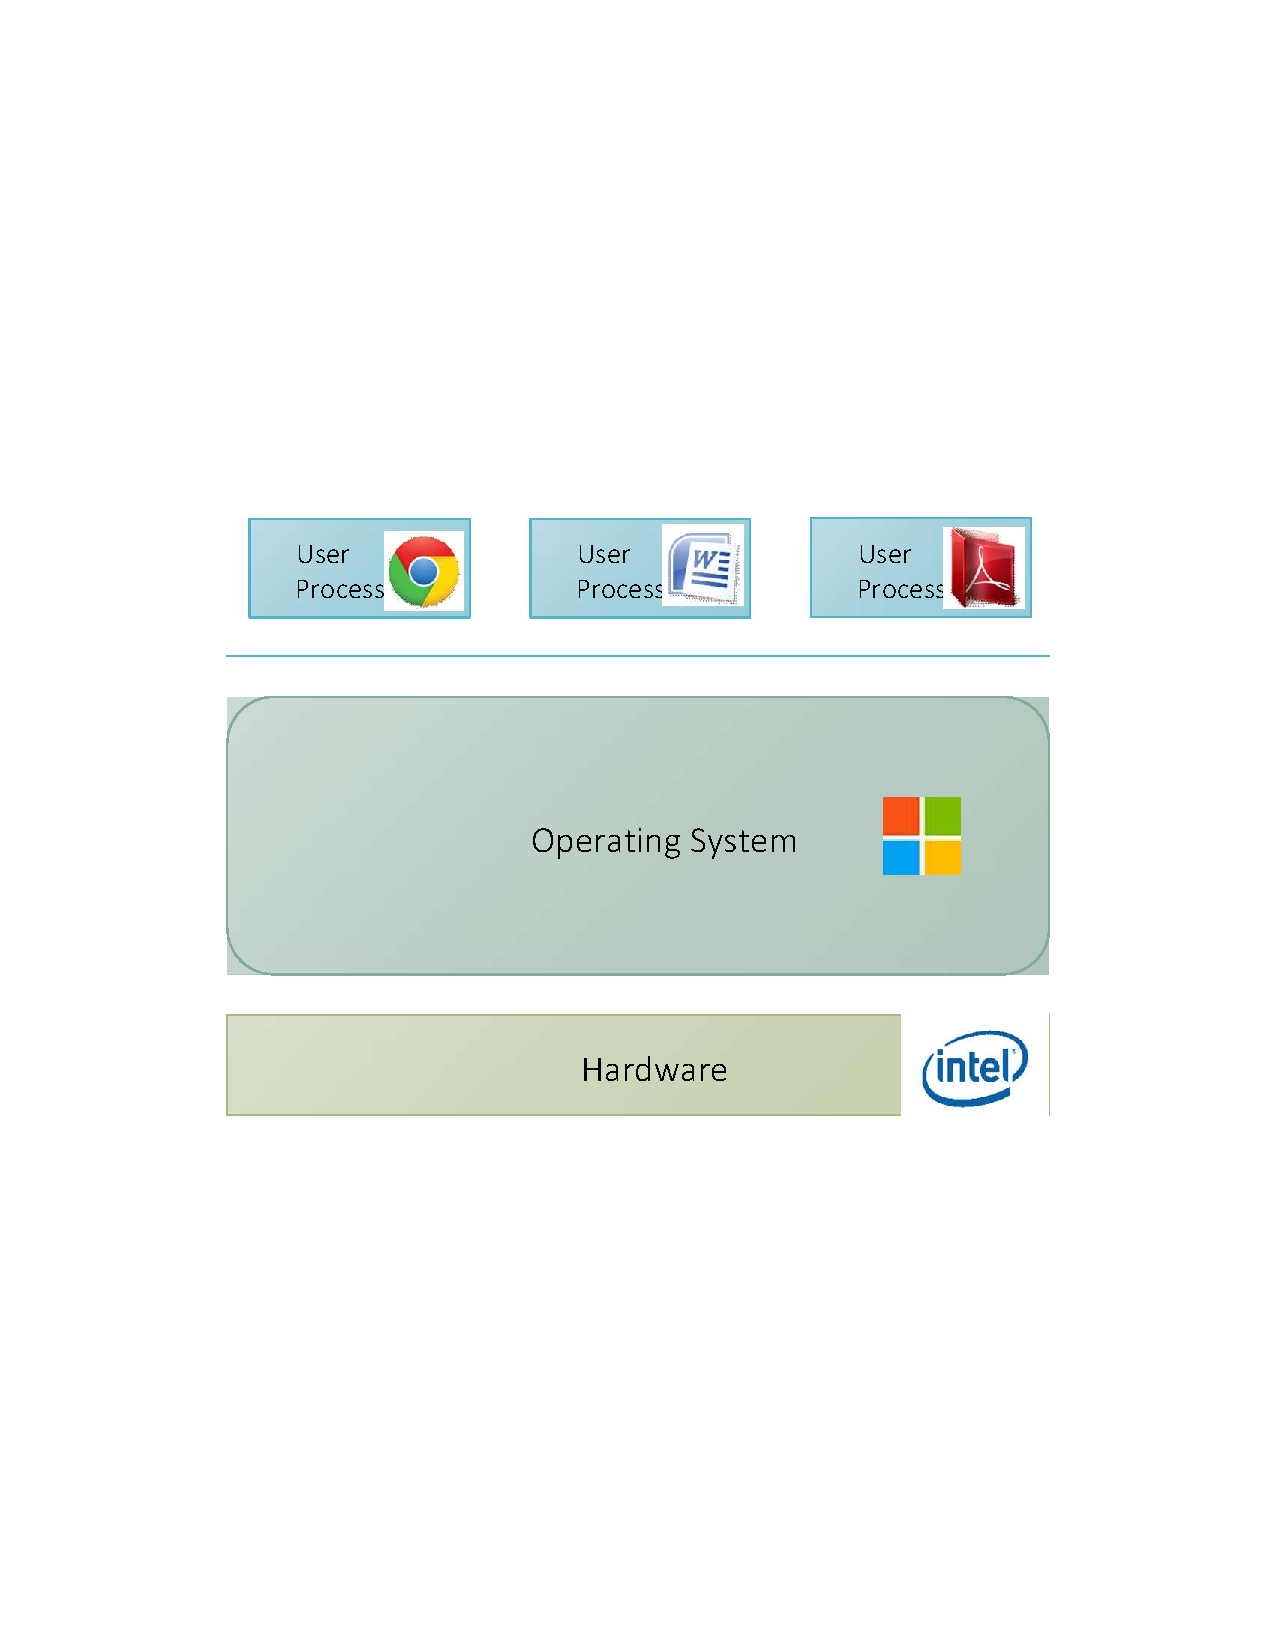
\includegraphics[scale=.25]{virtualization}
	\caption{Virtualization}
	\label{fig:Virtualization}
	\end{subfigure}
    \caption{Comparision of a non-virtualized system and a virtualized system}\label{fig:Kernel space}
\end{figure}

\subsection{Hypervisors}
A hypervisor is a piece of computer software, firmware, or hardware that creates and runs virtual machines. Operating system virtualization is achieved by inserting a VMM between the guest operating system and the underlying hardware. Most of the literature treats VMM and hypervisors synonymously. However, whereas a VMM is a software layer specifically responsible for virtualizing a given architecture, a hypervisor is an operating system that manages VMM. This operating system may be a general purpose one, such as Linux, or it may be developed specifically for the purpose of running virtual machines~\cite{Agesen:2010:EXV:1899928.1899930}.

A computer on which a hypervisor is running one or more virtual machines is defined as a host machine. Each virtual machine is called a guest machine. Multiple instances of a variety of operating systems share the virtualized hardware resources. Among widely known hypervisors are Xen~\cite{barham2003xen, Chisnall:2007:DGX:1407351}, KVM~\cite{Habib:2008:VK:1344209.1344217, kivity2007kvm}, VMware ESXi~\cite{Agesen:2010:EXV:1899928.1899930} and VirtualBox~\cite{camargos2008virtualization}.

There are two types of hypervisors~\cite{Popek:1974:FRV:361011.361073}
\begin{itemize}
\item Type 1 hypervisors are also called native hypervisors or bare metal hypervisors. Type 1 hypervisors run directly on the host's hardware and manage guest operating systems. Type 1 hypervisors represent the classic implementation of virtual-machine architectures such as SIMMON, and CP/CMS. Modern equivalents include Oracle VM Server for SPARC, Oracle VM Server, the Xen hypervisor~\cite{barham2003xen}, VMware ESX/ESXi~\cite{Agesen:2010:EXV:1899928.1899930} and Microsoft Hyper-V.
\begin{figure}[!ht]
\centering
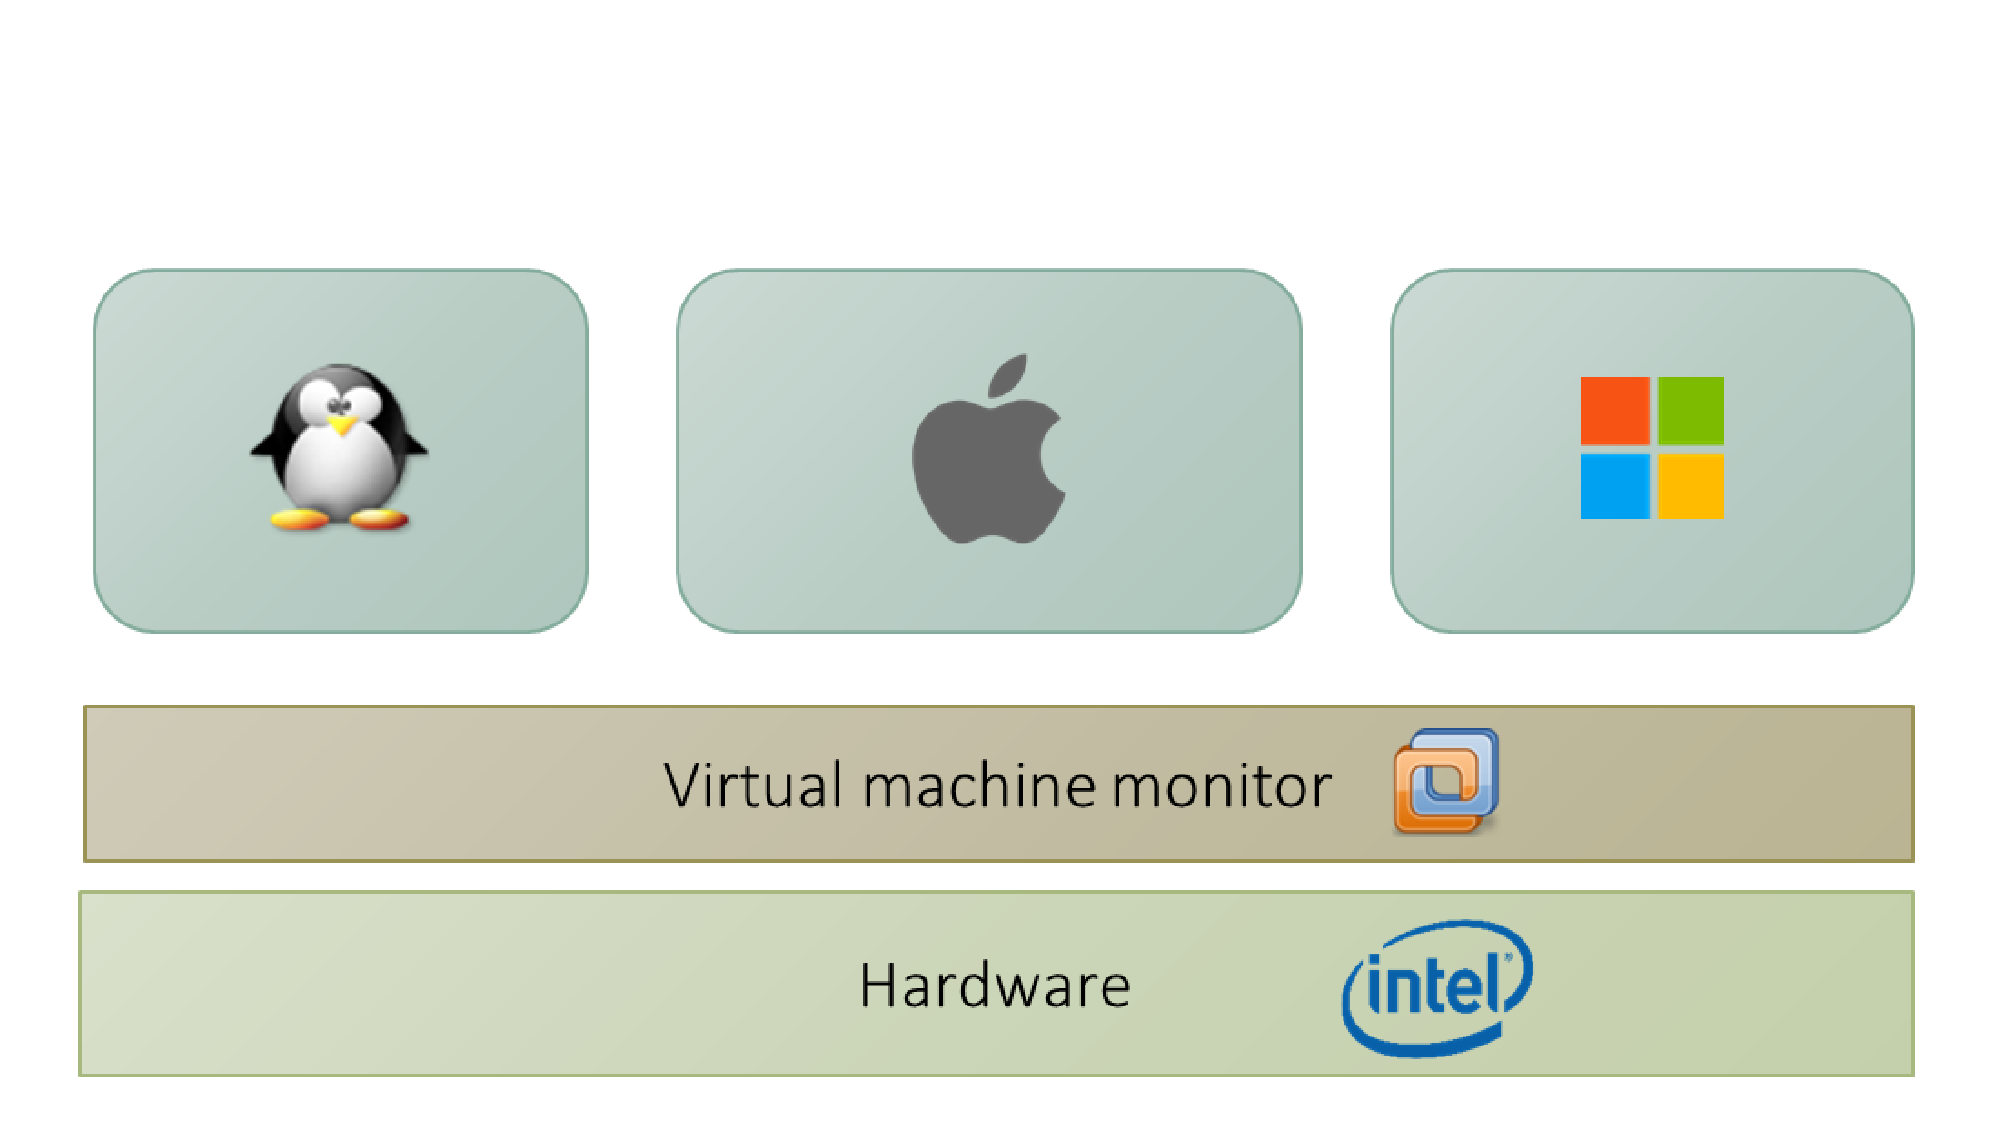
\includegraphics[scale=.35]{type1}
\caption{Type 1 hypervisors}
\label{Type 1 hypervisor}
\end{figure}
\item Type 2 hypervisors are also called hosted hypervisors. Type 2 hypervisors run within a conventional operating-system environment. VMware Workstation and VirtualBox are some examples of Type 2 hypervisors~\cite{Sugerman:2001:VID:647055.715774, camargos2008virtualization}.
\begin{figure}[!ht]
\centering
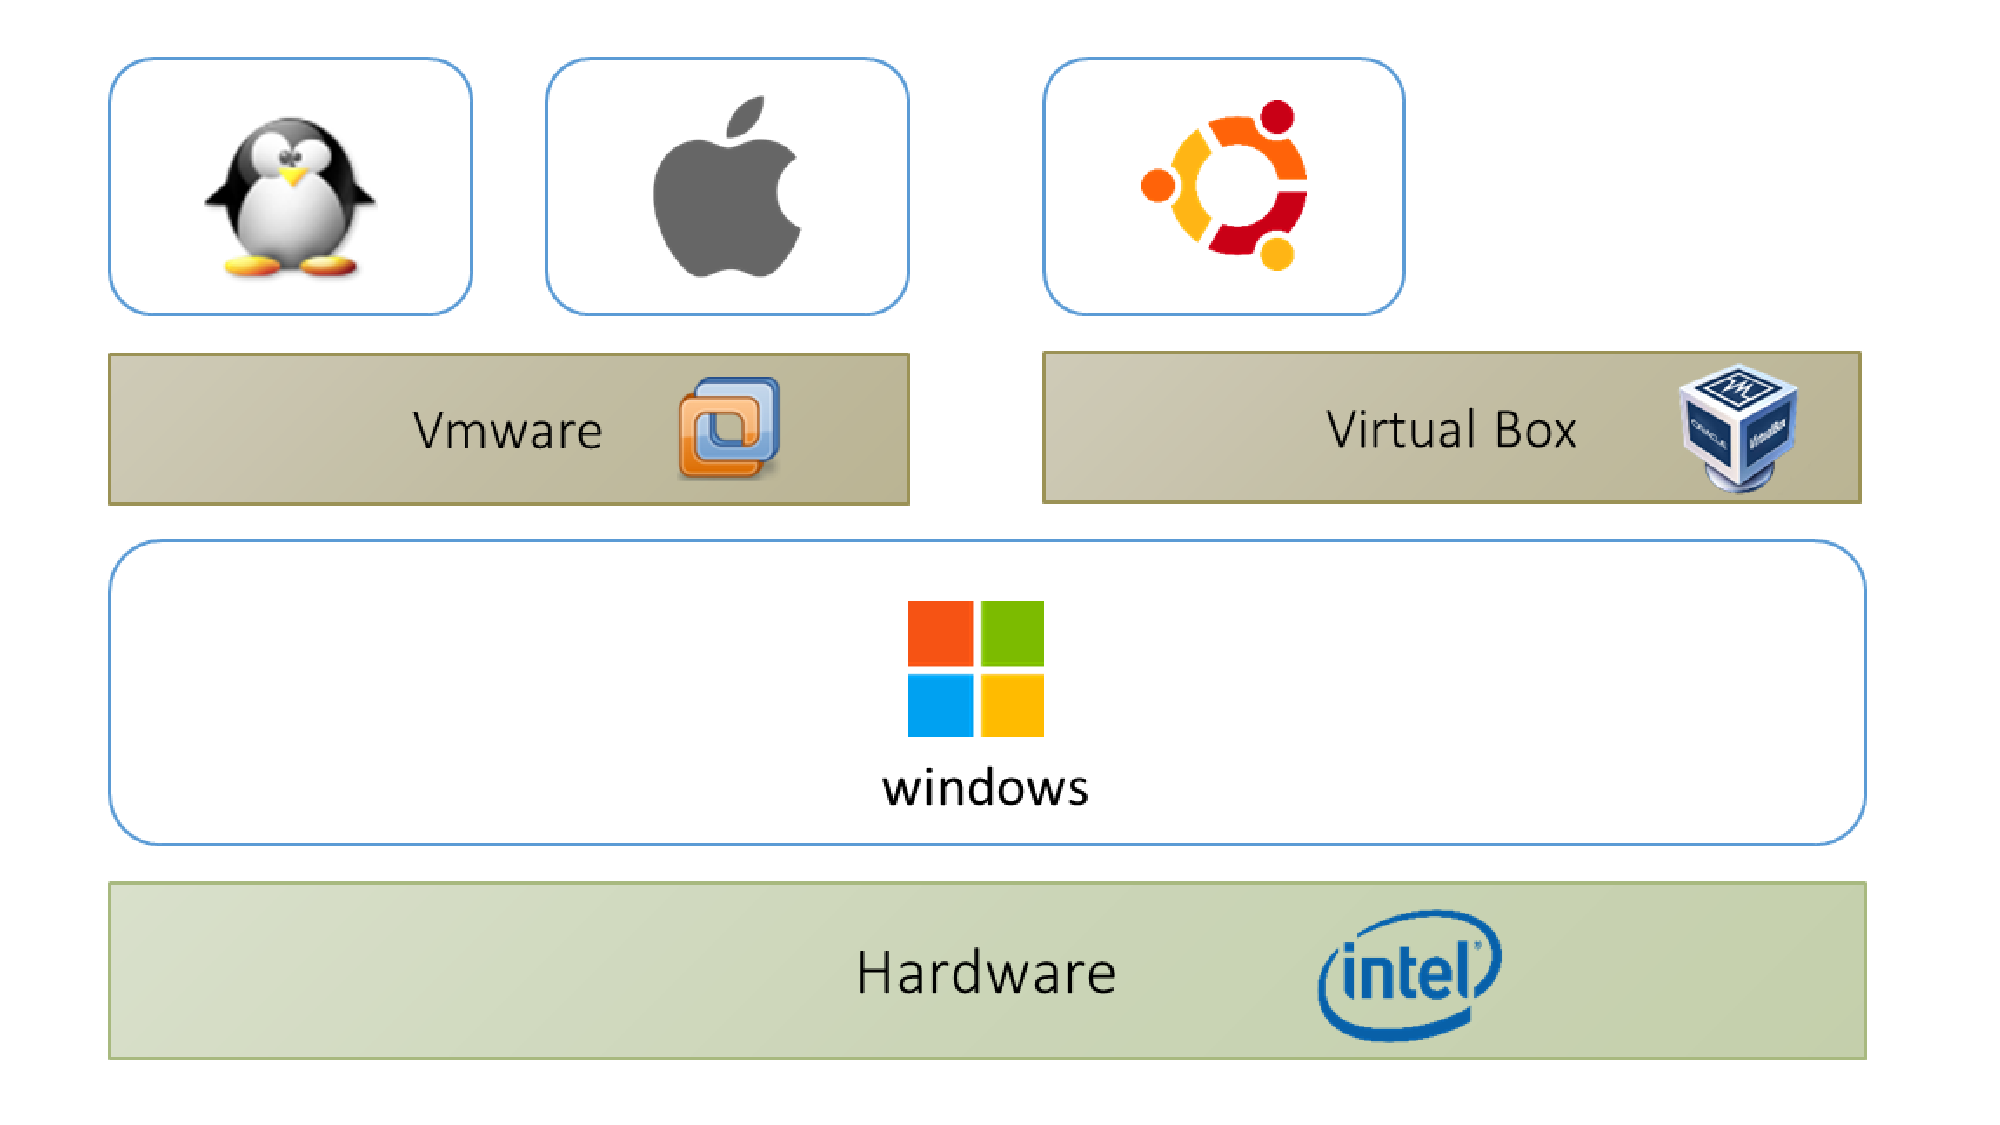
\includegraphics[scale=.4]{type2}
\caption{Type 2 hypervisors}
\label{fig:Type 2 hypervisor}
\end{figure}
\end{itemize}

\subsection{Xen Hypervisor}
Xen~\cite{barham2003xen} is a widely known Type 1 hypervisor that allows the execution of virtual machines in guest domains~\cite{king2003operating}. Xen runs guest operating systems in environments known as domains. \texttt{Domain 0} is the first guest to run, and has elevated privileges. Xen loads a \texttt{domain 0} guest kernel during boot. Unprivileged domain is called \texttt{domain U}. The Xen hypervisor does not include device drivers. Device management is included in privileged \texttt{domain 0}. \texttt{Domain 0} uses the device drivers present in the guest operating system. The other domains access devices using a split device driver architecture, in which a frontend driver in a guest domain communicates with a backend driver in \texttt{domain 0}.

Figure~\ref{xen-split2} shows how an application running in a \texttt{domain U} guest writes data on a physical device. Xen provides an inter-domain memory sharing API accessed through the guest kernel extensions and an interrupt-based inter-domain signaling facility called event channels to implement the efficient inter-domain communication. Split device driver model uses memory sharing APIs to implement I/O device ring buffers to exchange requests and responses across domains and use event channels to send virtual interrupt when requests and responses are shared. 

Consider the example shown in Figure~\ref{xen-split2}. First, write request is sent to the file system. After that the frontend driver puts the data into memory which is shared between \texttt{domain 0} and \texttt{domain U}. The other half of the split device driver called the backend, running in the \texttt{domain 0} guest, reads the data from the buffer and sends it to the real device driver. The data is then written to the actual physical device~\cite{Chisnall:2007:DGX:1407351}.

\begin{figure}[!h]
\centering
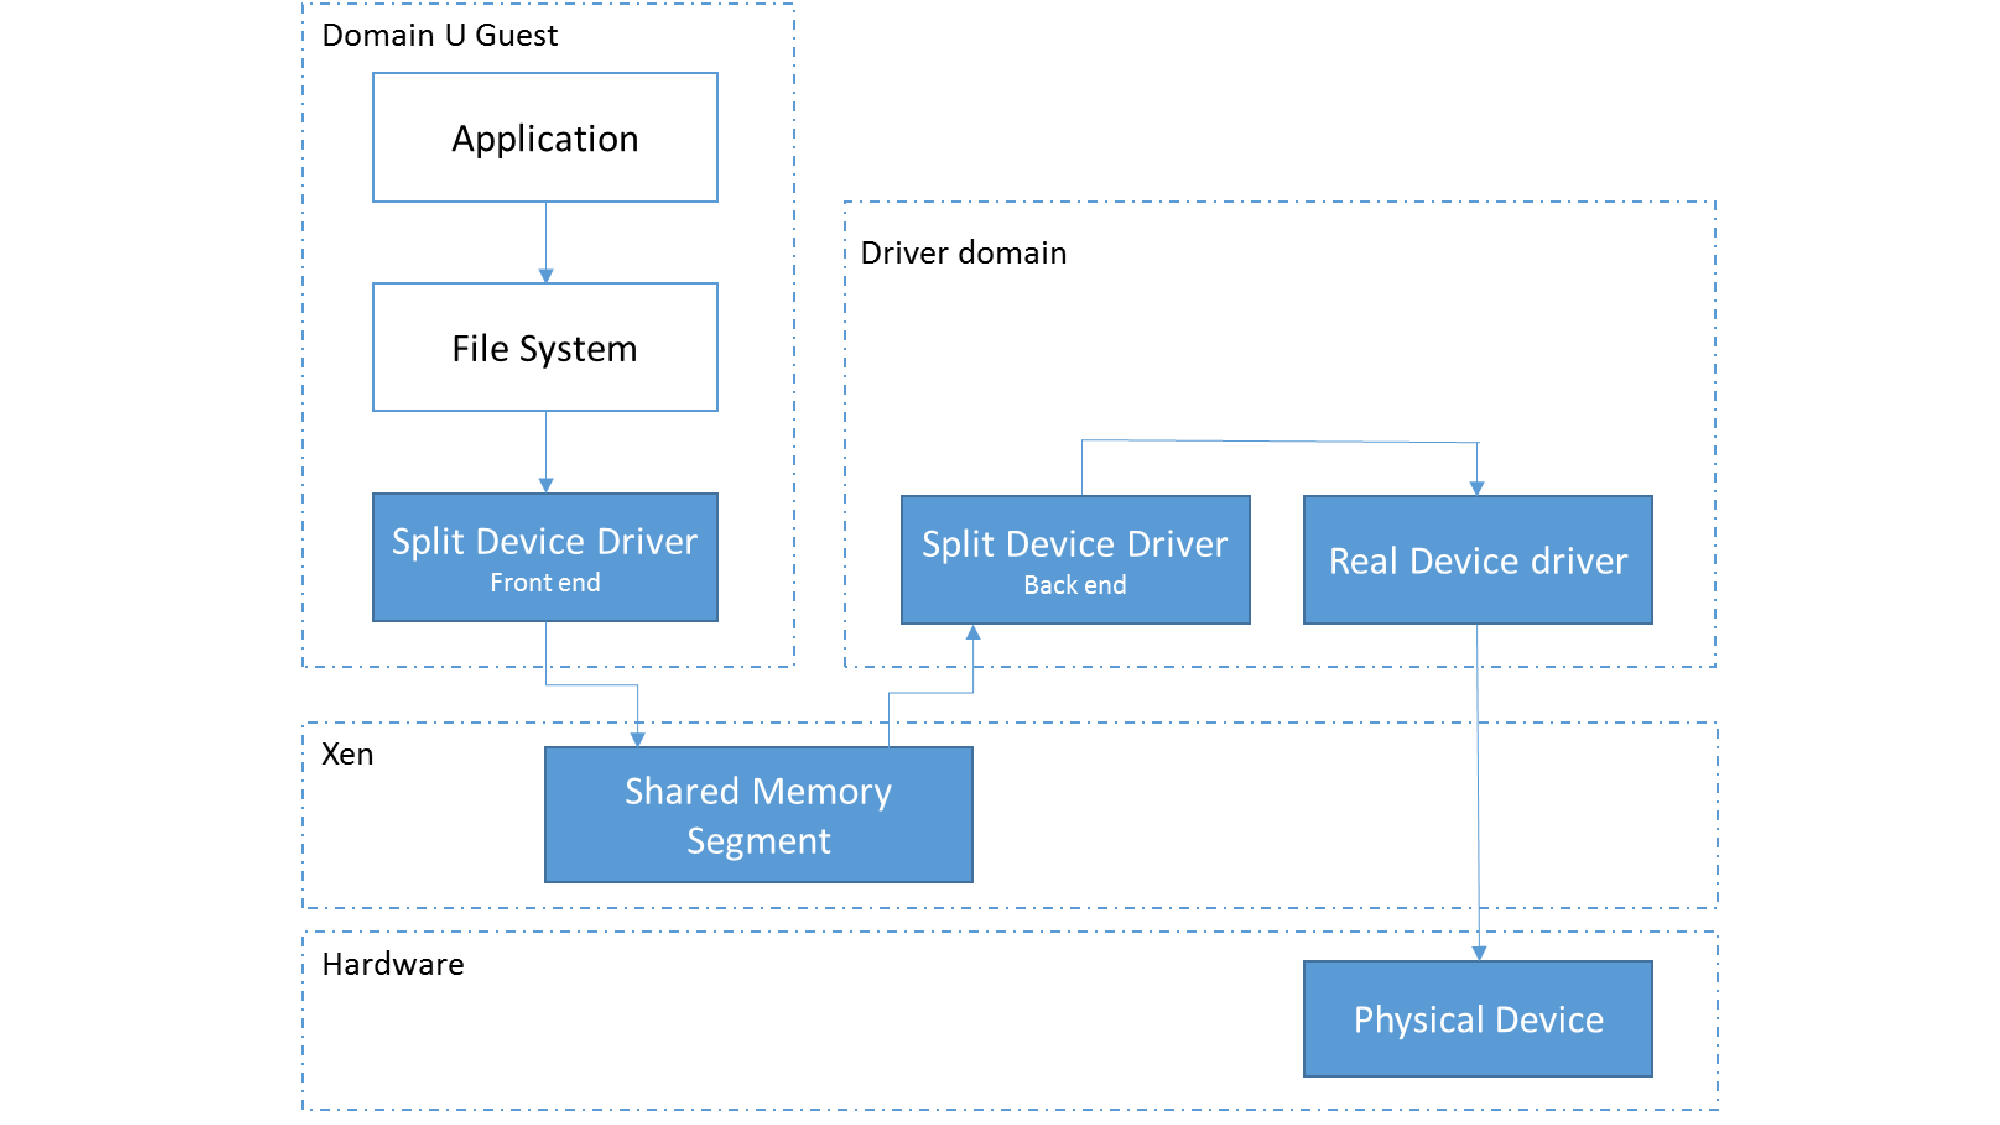
\includegraphics[scale=.50]{xen-split-fs}
\caption{Xen split device driver}
\label{xen-split2}
\end{figure}
\begin{figure}[!h]
\centering
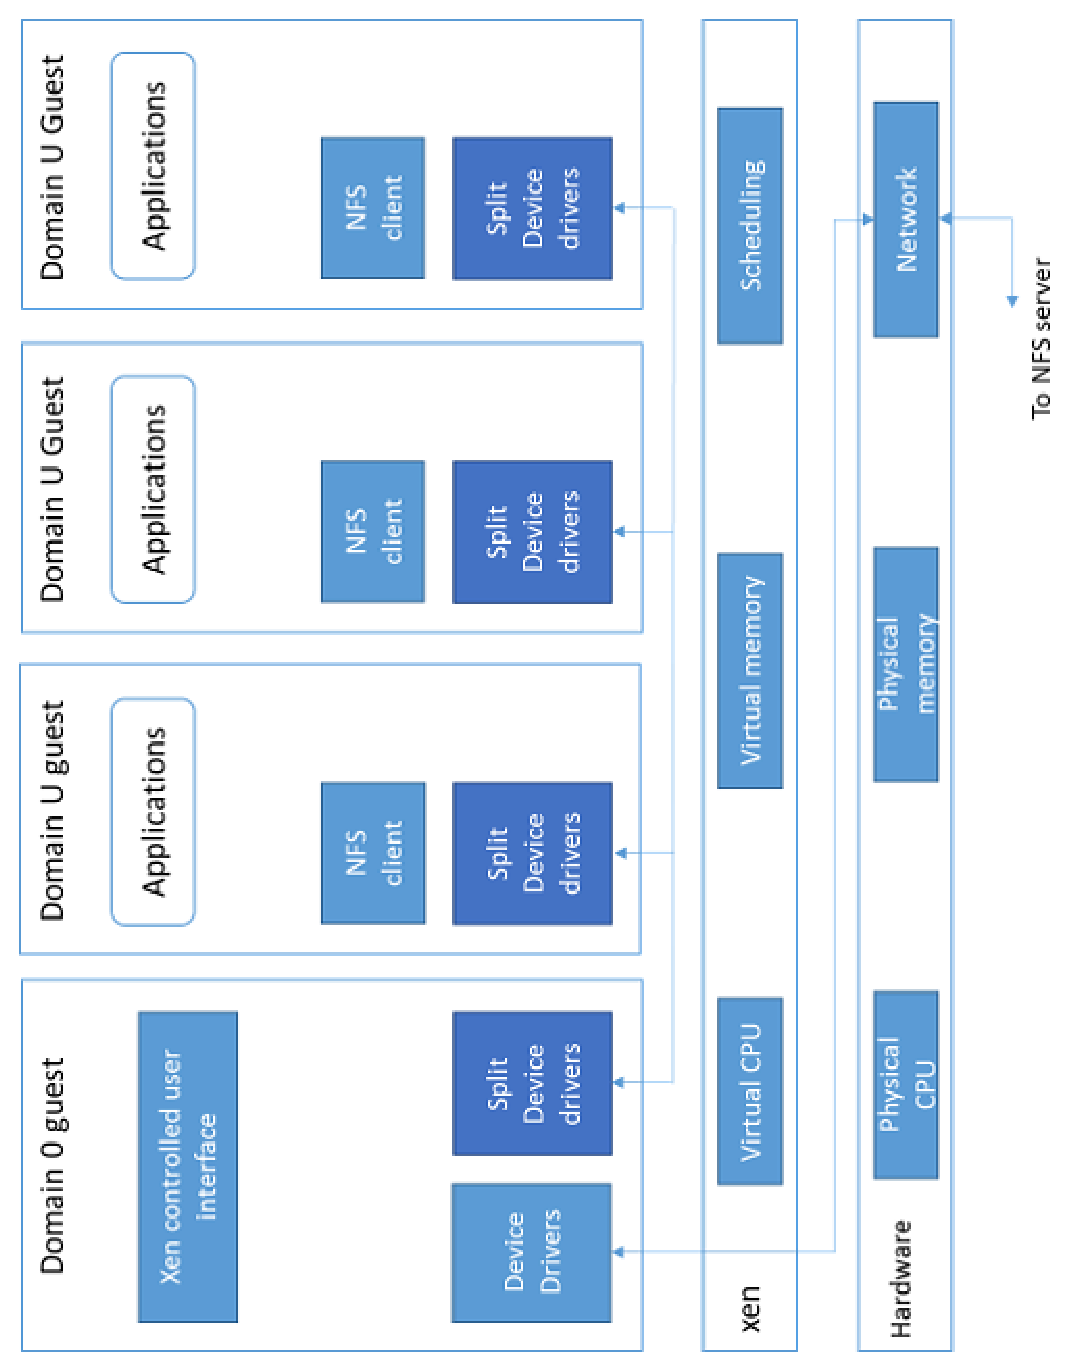
\includegraphics[scale=.50]{xen}
\caption{Xen}
\label{xen}
\end{figure}

\subsubsection*{Hypercalls and Events}
Hypercalls and event channels are the two mechanisms that exist for interactions between the Xen hypervisor and domains. A hypercall is a software trap from a domain to the Xen hypervisor, just as a syscall is a software trap from an application to the kernel~\cite{hypercall}. Domains use hypercalls to request privileged operations like updating pagetables. 

An event channel is to the Xen hypervisor as a signal is to an operating system. An event channel is used for sending asynchronous notifications between domains. Event notifications are implemented by updating a bitmap. After scheduling pending events from an event queue, the event callback handler is called to take appropriate action. The callback handler is responsible for resetting the bitmap of pending events and responding to the notifications in an appropriate manner. A domain may explicitly defer event handling by setting a Xen readable software flag: this is analogous to disabling interrupts on a real processor. Event notifications can be compared to traditional UNIX signals acting to flag a particular type of occurrence. For example, events are used to indicate that new data has been received over the network, or used to notify that a virtual disk request has completed. 

\subsubsection*{Data Transfer: I/O Rings}
\label{subsec:io rings}
Hypervisors introduce an additional layer between a guest OS and I/O devices. Xen provides a data transfer mechanism that allows data to move vertically through the system with minimum overhead. 
\begin{figure}[!ht]
\centering
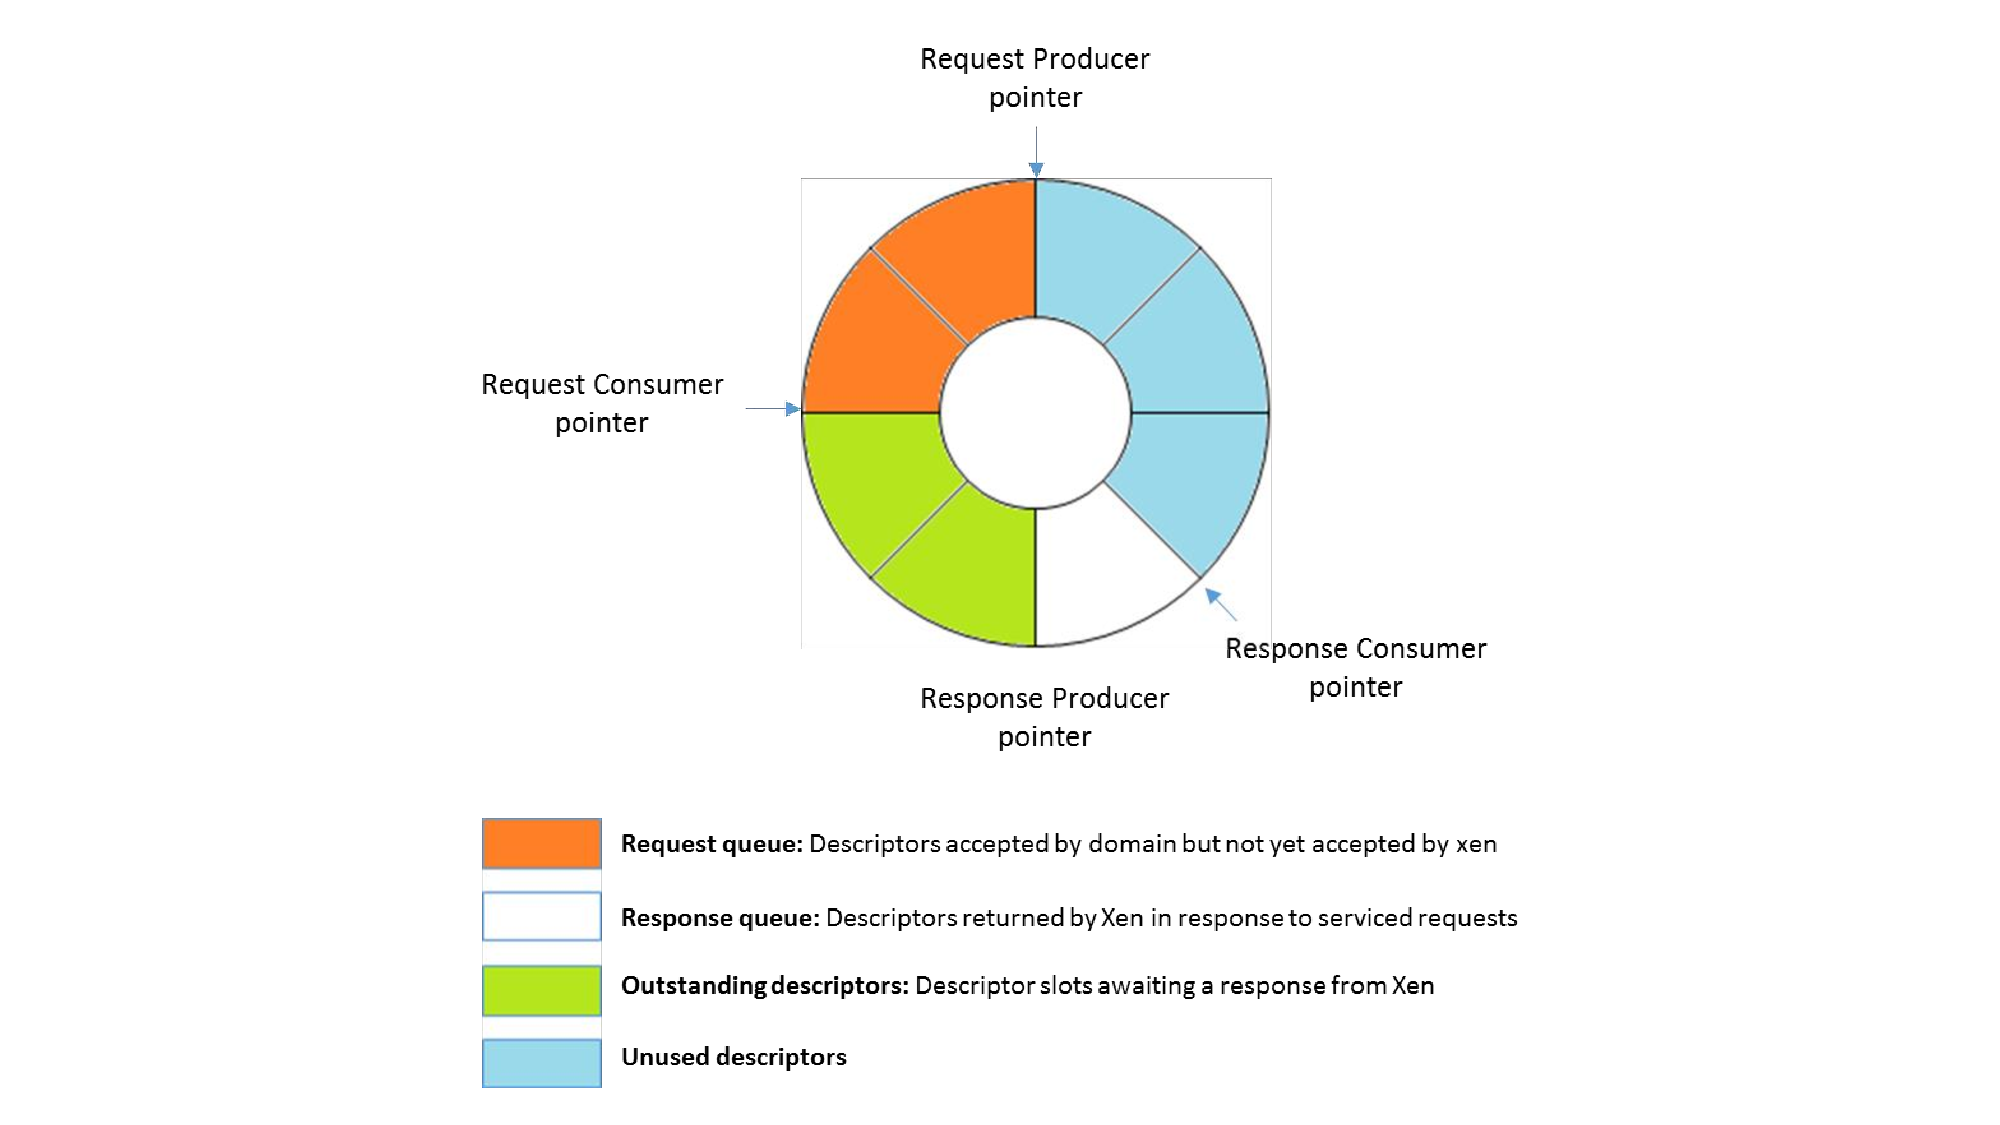
\includegraphics[scale=.5]{IObuffer}
\caption{Ring I/O buffer}
\label{fig:Ring buffer}
\end{figure}

Figure~\ref{fig:Ring buffer} shows the structure of an I/O descriptor ring. An I/O descriptor ring is a circular queue of descriptors allocated by a domain. These descriptors do not contain I/O data. I/O data buffers are allocated separately by the guest OS and are indirectly referenced by these I/O descriptors. Access to an I/O ring is based on two pairs of producer-consumer pointers.
\begin{enumerate}
\item Request producer pointer: A producer domain places requests on a ring by advancing the request producer pointer. 
\item Request consumer pointer: A consumer domain removes these requests by advancing the request consumer pointer.
\item Response producer pointer: A Consumer domain places responses on a ring by advancing the response producer pointer. 
\item Response consumer pointer: A producer domain removes these responses by advancing the response consumer pointer.
\end{enumerate} 

Notifications are not sent for each individual request and response. A domain can enqueue multiple requests and responses before notifying the other domain. This allows each domain to tradeoff between latency and throughput.
\begin{figure}[!ht]
\centering
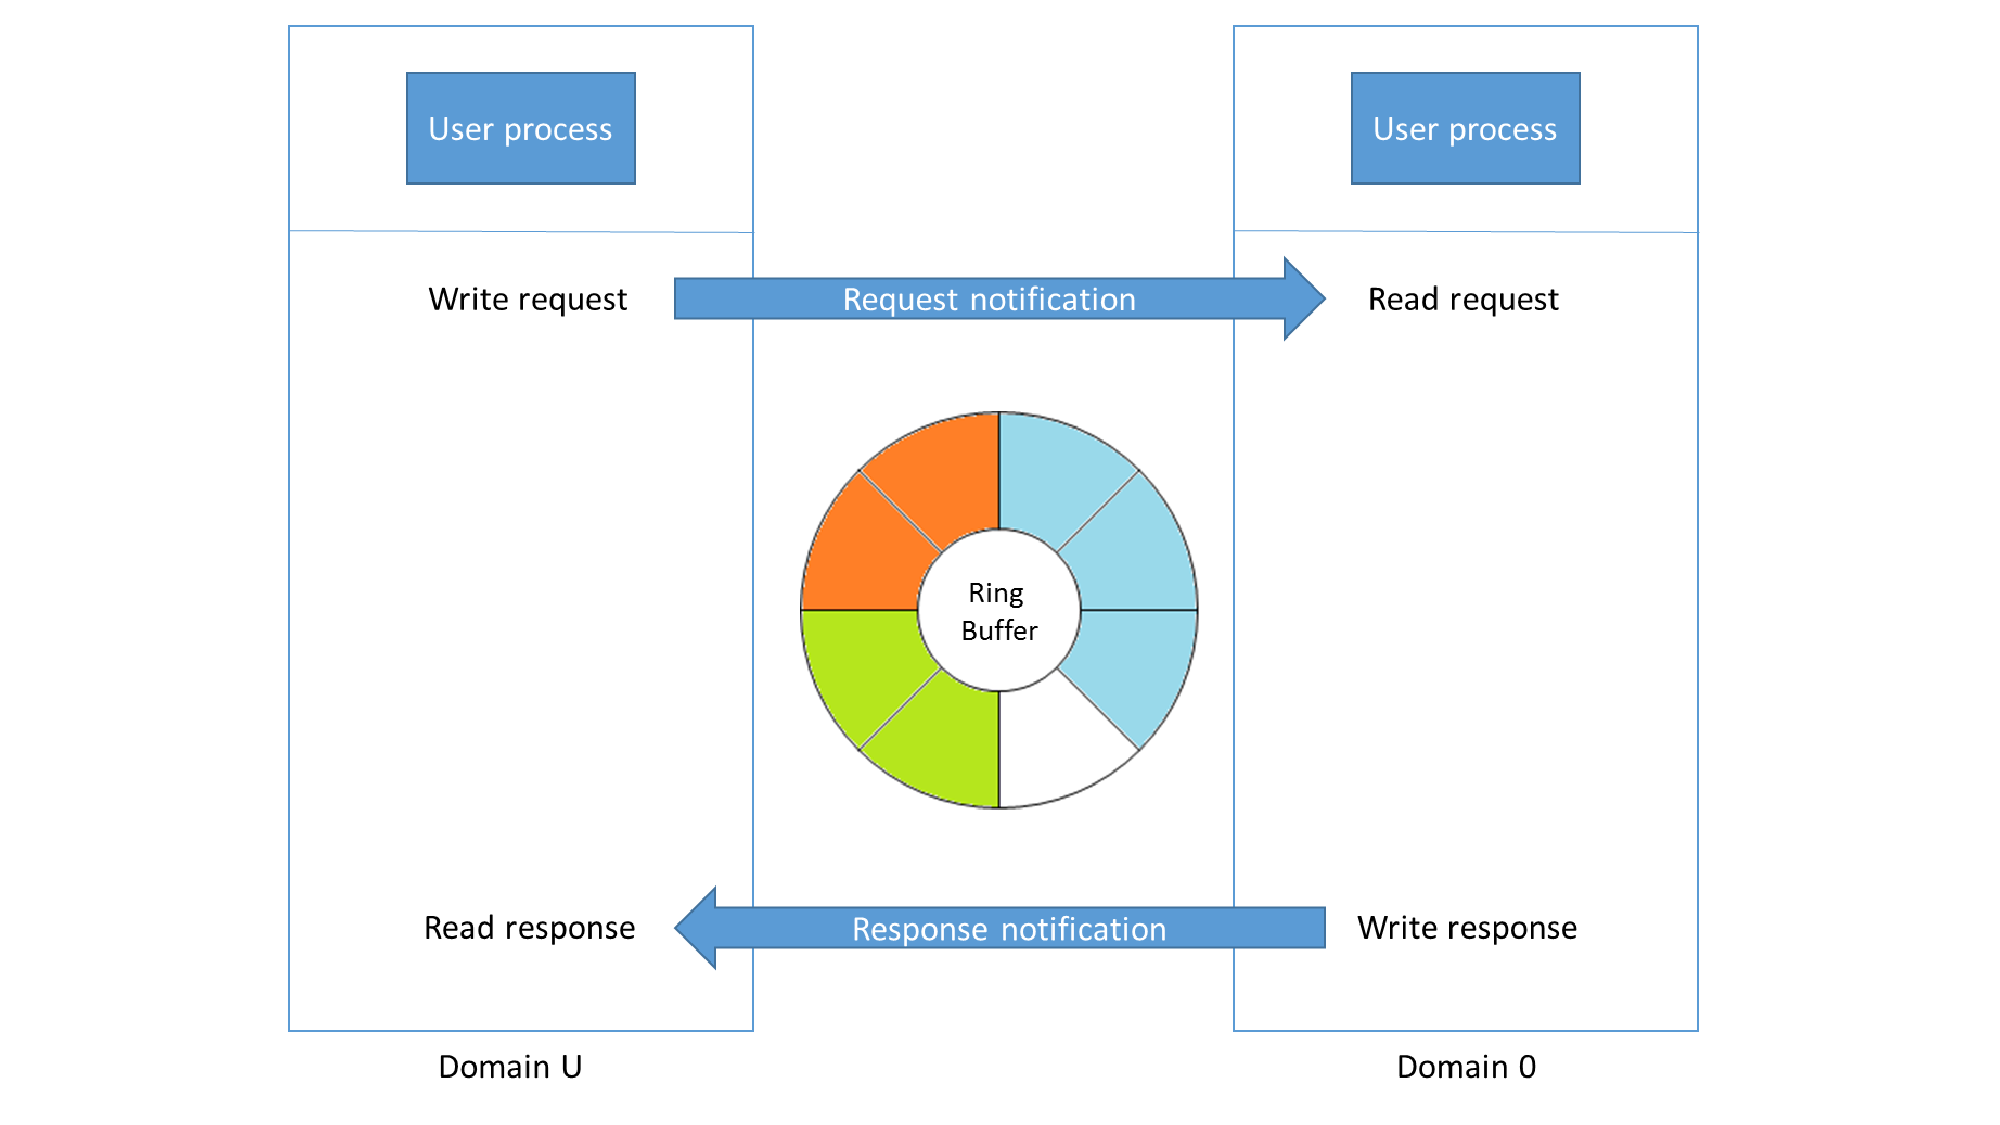
\includegraphics[scale=.5]{IObuffer2}
\caption{Ring I/O buffer}
\label{fig:Ring buffer}
\end{figure}

\subsection*{Shared Pages}
\label{subsec:sharedpages}
\subsubsection*{Grant Table} 
Grant tables are a mechanism provided by the Xen hypervisor for sharing and transferring memory between the domains. It is an interface for granting foreign access to machine frames and sharing memory between unprivileged domains. Each domain has its own grant table data structure, which is maintained by the Xen hypervisor. The grant table data structure is used to verify the access permissions other domains have to pages allocated by a domain~\cite{granttable}.

\subsubsection*{Grant References}
Grant table entries are referred to as grant references. A grant reference entry contains all necessary details about a shared page. 

The Xen hypervisor virtualizes the physical memory. In Xen hypervisor, a domain requires the machine address of a frame in order to share a memory with other domain. It is not possible to know the machine address of a frame for a domain. A grant reference removes the dependency on the real machine address in order to share a page and makes it possible to share the memory between domains.\cite{Chisnall:2007:DGX:1407351, barham2003xen, granttable} 
\ifbool{toShowBibliography}{\bibliography{references}}{}


% System Overview/Architecture
\chapter{System Introduction}
\markright{Sushrut Shirole \hfill Chapter 3. System Introduction \hfill}

\section{Design Goal}\label{sec:goals}
The goal of the IDDR system is to provide full isolation between a device driver and the monolithic kernel and at the same time avoid modifications to the device driver code. The goal of the thesis is to minimize the performance penalty because of the communication between the domains. In the thesis, we explore opportunities to minimize the overhead of the communication module in the IDDR system.

\subsection*{Performance Improvement}
The IDDR system is a re-implementation of the Xen's isolated driver domain. Even though the IDDR system provides better robustness for the operating system, it deteriorates the performance. The reasons for the performance deterioration is due to the introduction of hypervisor, data copy overhead or overhead of communication between the domains. 

\paragraph{Hypervisor Layer: } The IDDR system uses Xen hypervisor as a virtualization platform. Xen hypervisor is a Type 1 hypervisor. A type 1 hypervisor runs directly on the host's hardware. It runs between the operating system and the hardware. In Xen, the hypervisor runs in ring 0, while guest OS runs in ring 1 and applications run in ring 3. For hardware access, the guest OS has to go through the hypervisor, which degrades the performance of the system

\paragraph{Copy Overhead: } For data intensive operations such as read and write, the IDDR system transfers data between the hardware and the driver domain. It also transfers the same data between the driver domain and the application domain. The extra copy from the driver domain to the application domain is also one of the reasons for the performance degradation of the system. 

\paragraph{Communication Channel Overhead: } The IDDR system runs a device driver in a separate domain called the driver domain. The application domain and the driver domain communicate with each other in order to send requests and get responses from the device driver. The communication between domains add an overhead to the system performance. Our goal is to minimize the overhead during communication between the driver domain and the application domain.

\section{Isolated Device Driver Properties}
\label{sec:properties}
This section covers the properties of the base IDDR system. As we are explore the opportunities to improve the performance of the base IDDR system, it is necessary that these properties are not compromised.

\subsection*{Strong isolation}
One of the main properties of the IDDR system is strong isolation. The IDDR system adds an extra layer of isolation in the design which provides fault isolation between the kernel and the device driver. The strong isolation also adds the ability to manage device drivers independently, thus, increasing the availability of the system during maintenance of a device driver.

\subsection*{Compatibility and Transparency} 
The extension of existing OS structures usually results in a large number of broken applications. As a specific example, in the microkernel architecture the functional units of an OS were divided into discrete parts in order to achieve the isolation between the kernel components. As a result, the APIs visible to applications were changed~\cite{Heiser06arevirtualmachine}, which broke the large number of applications. In order to provide compatibility with applications, many microkernel architectures provided an emulation layer~\cite{Heiser06arevirtualmachine} for the OSes. The IDDR system maintains compatibility between existing device drivers and applications.

\section{System overview}\label{overview}

Figure~\ref{fig:monolithic} shows the architectural overview of the modern operating system with a monolithic kernel and the architectural overview of the IDDR system is presented in Figure~\ref{fig:base IDDR system overview}.
\\[3mm]
\begin{figure}[!ht]
\centering
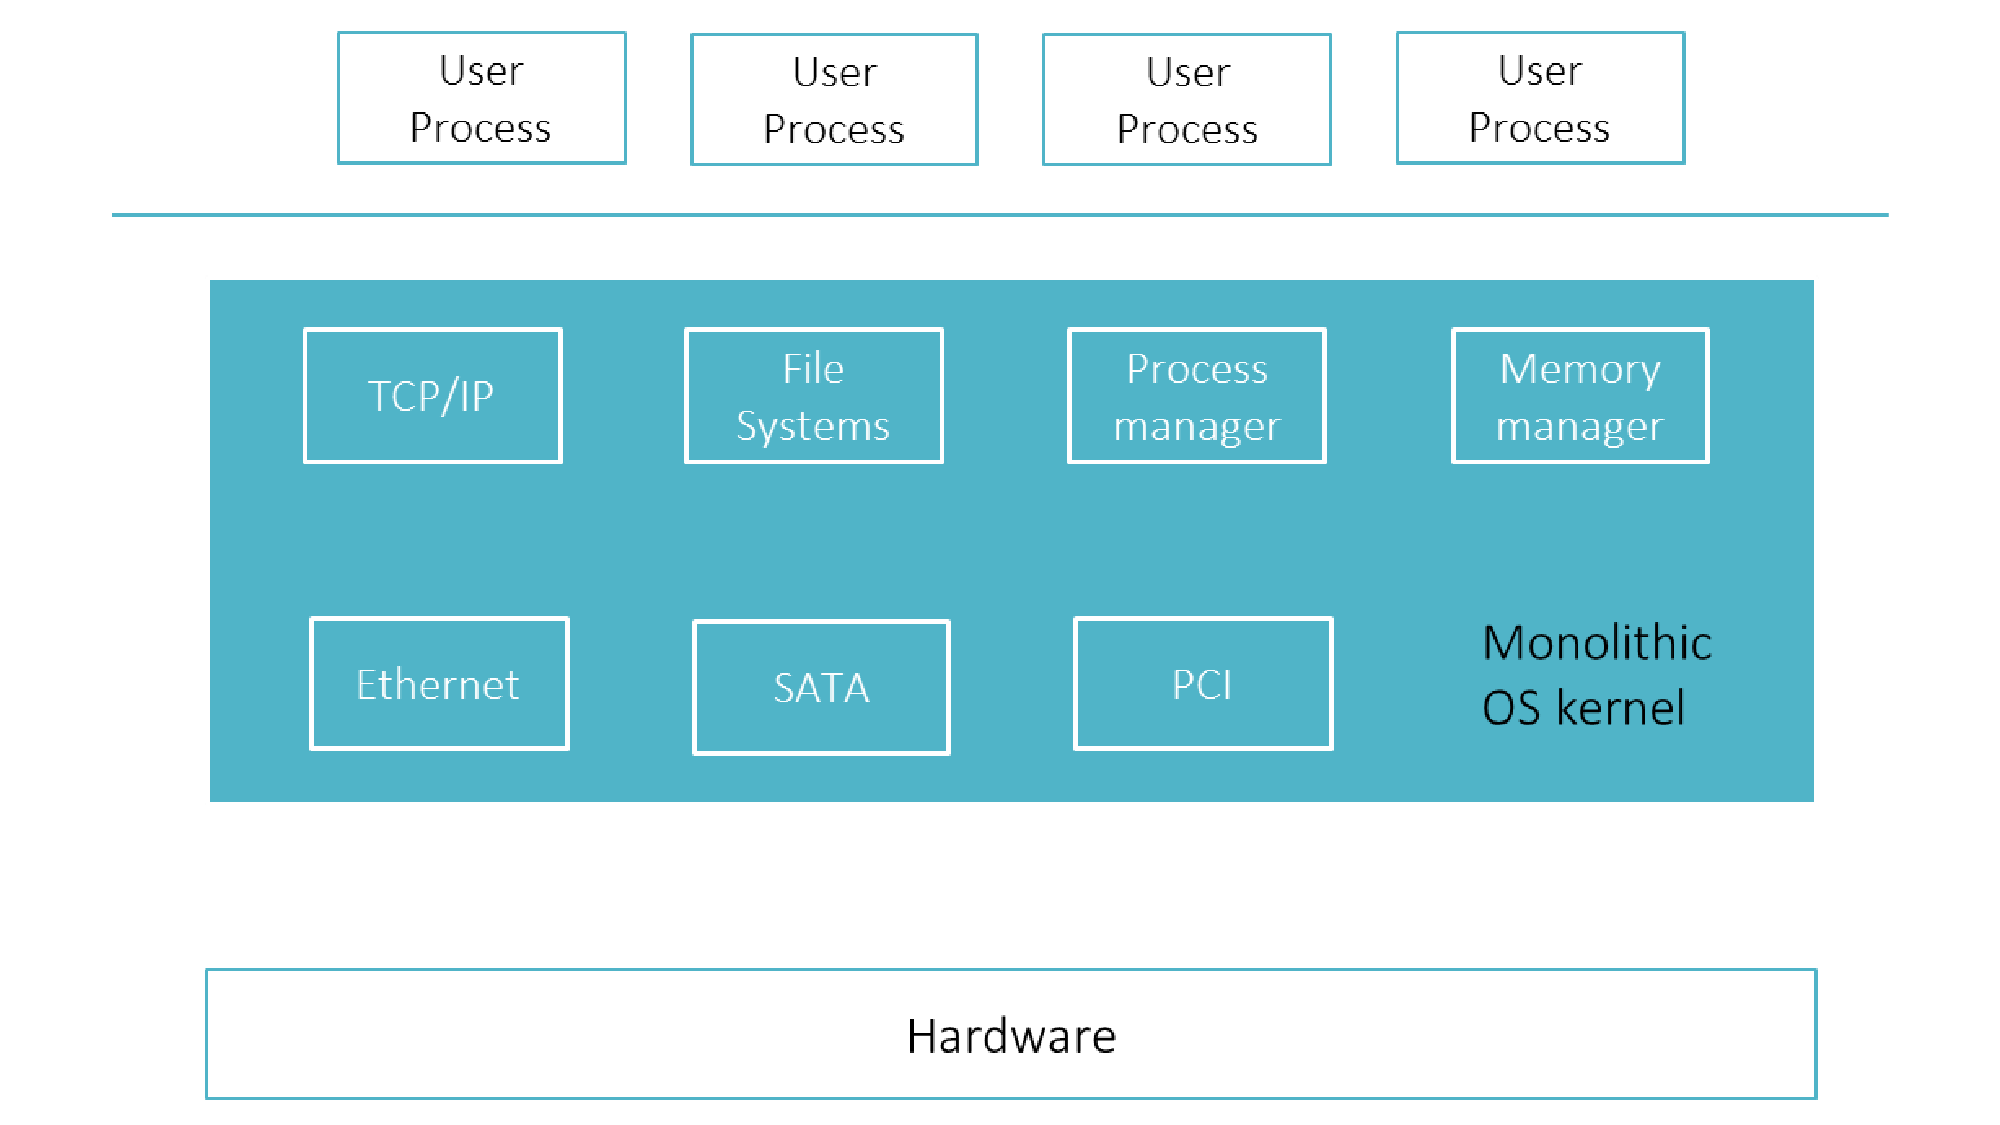
\includegraphics[scale=.5]{OSoverview}
\caption{Architectural overview of modern OS}
\label{fig:monolithic}
\end{figure}

\begin{figure}[!ht]
\centering
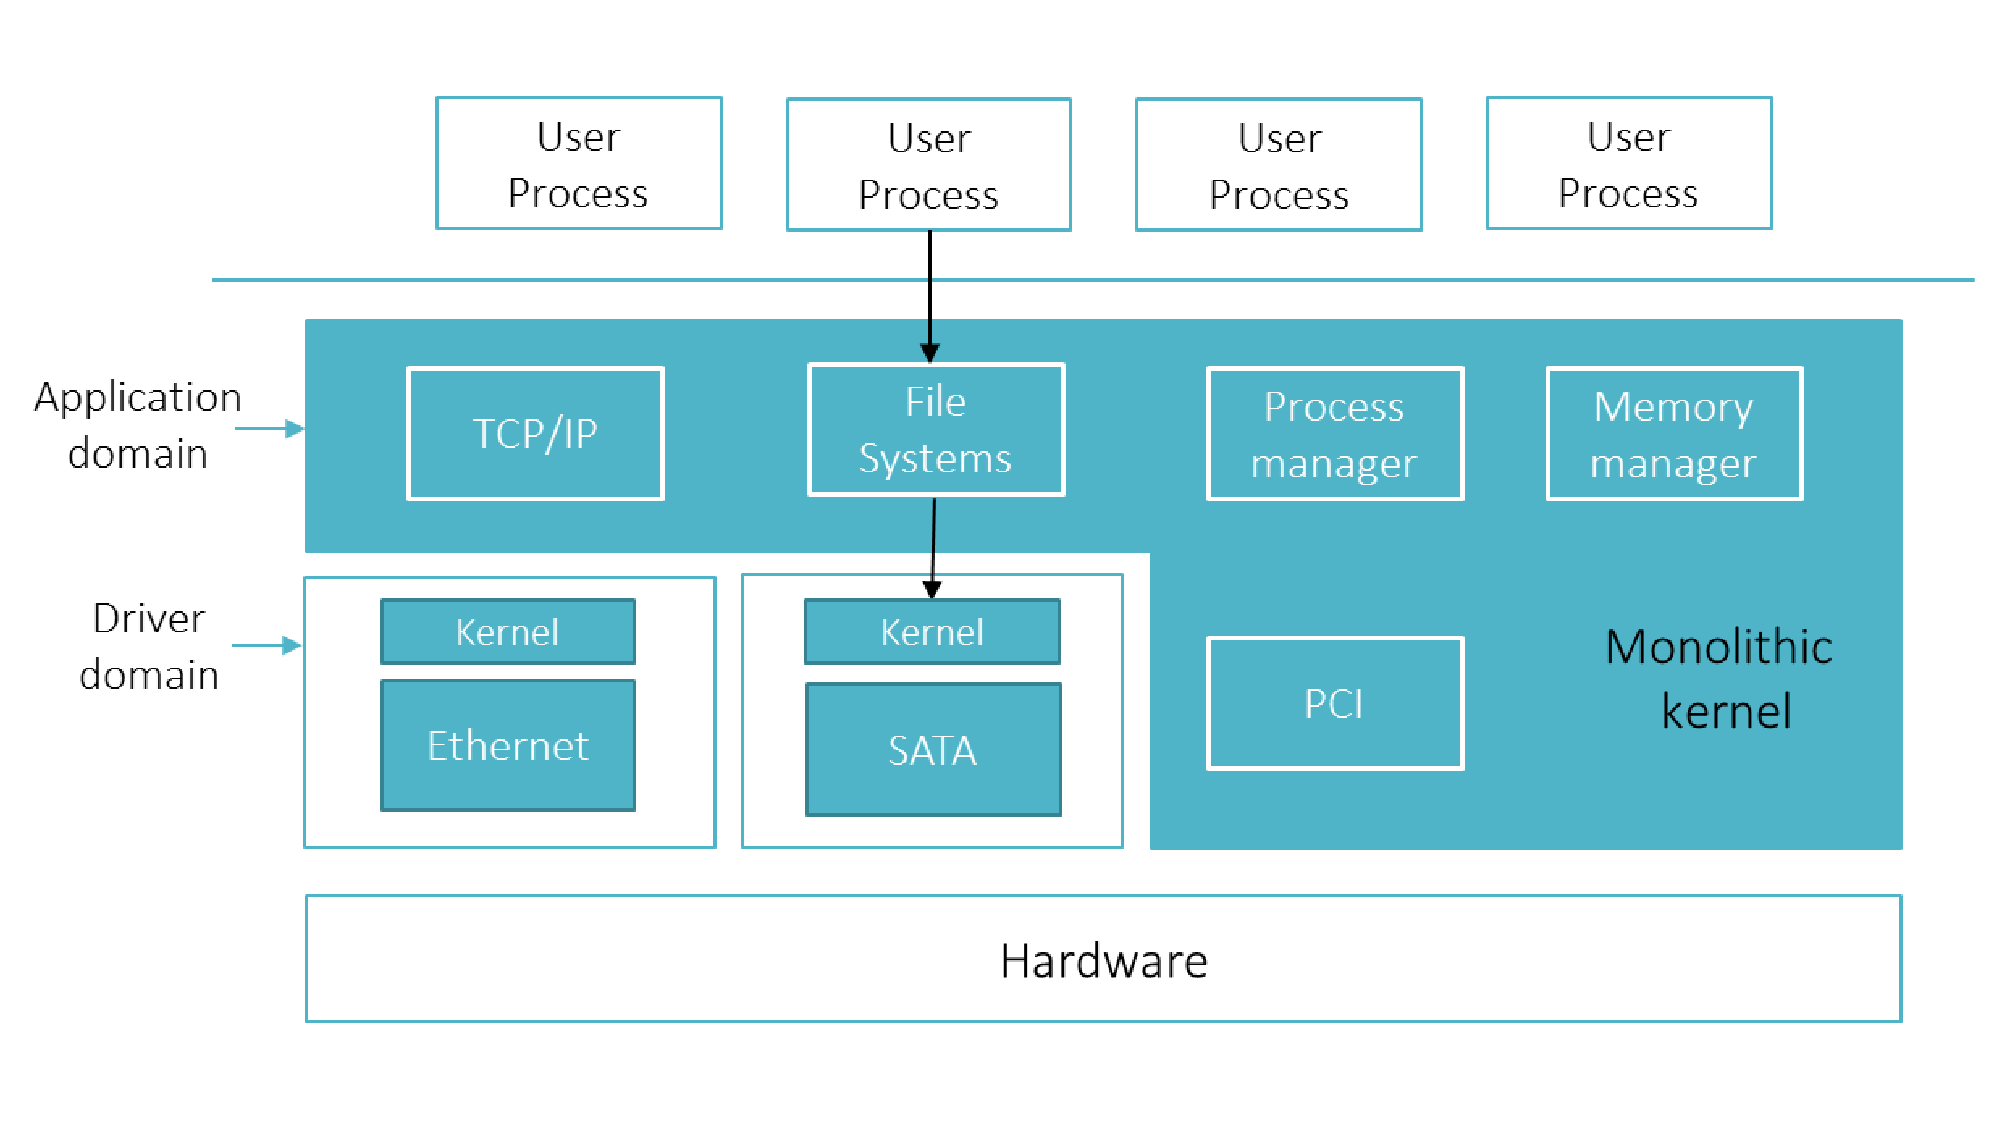
\includegraphics[scale=.5]{baseIDDRsystemoverview}
\caption{Architectural overview of the base IDDR system}
\label{fig:base IDDR system overview}
\end{figure}
The Figure~\ref{fig:base IDDR system overview} shows that the IDDR system partitions an existing kernel into multiple independent components. The user applications and Linux kernel run in a domain called as the \textit{application domain}. The device driver which needs to be isolated from the kernel, executes in the separate domain called as the \textit{driver domain}. Multiple domains run on a same hardware with the help of a VMM. User applications or kernel components access the hardware through the device driver domain.
\\[3mm]
As the section~\ref{sec:goals} describe the goal of the IDDR system is to provide the isolation between the device driver and the kernel. However a device driver is dependent on the kernel components such as a scheduler and memory management unit. In order to remove the dependency, the device driver runs closely with another instance of a kernel. Even though the dependency is removed, it is not possible to run multiple kernels over the common hardware without a virtual machine monitor. Thus, a VMM is introduced in the design to run multiple kernels on a common hardware. 

\section{System components}\label{components}
The section describes the 3 main components of the design - frontend driver, backend driver and communication module.
\begin{figure}[!ht]
\centering
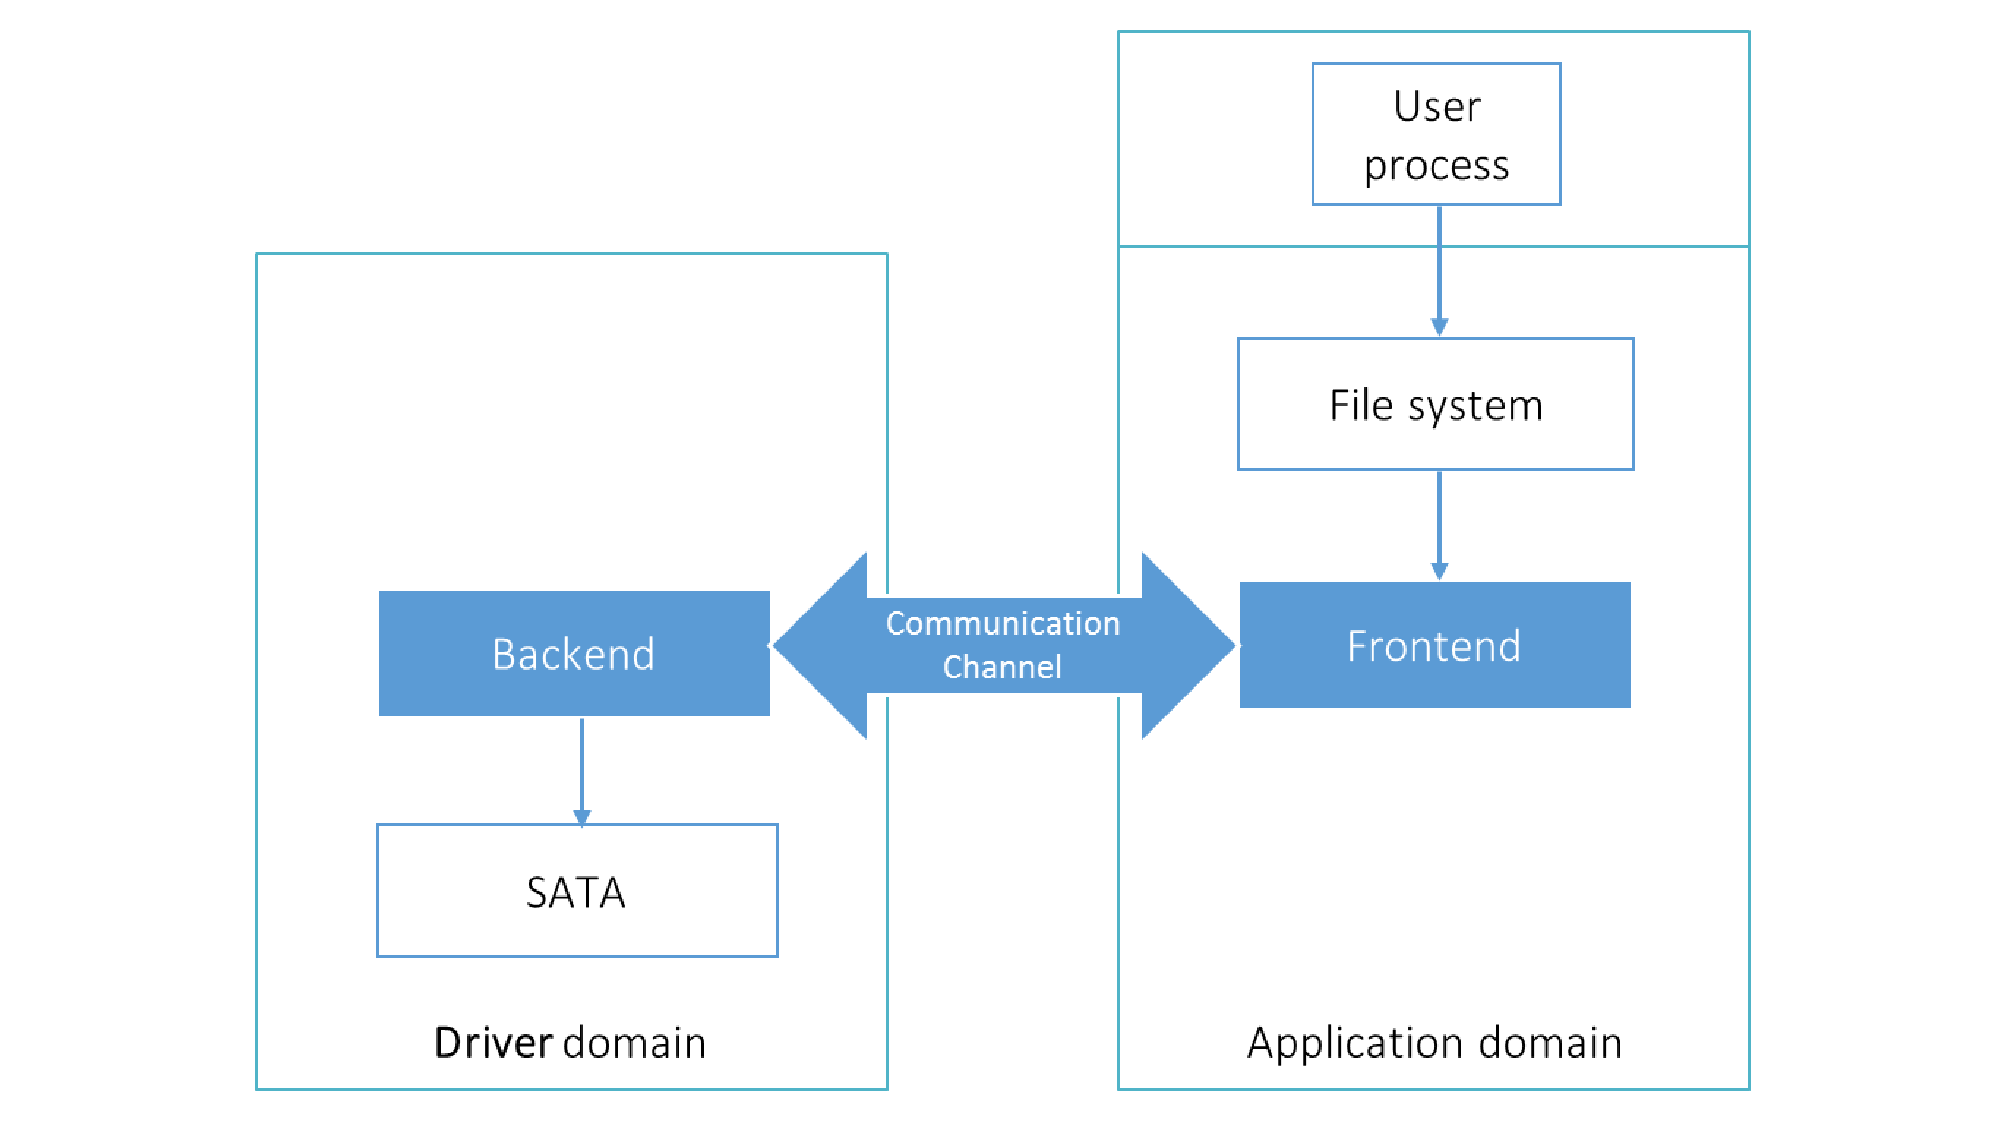
\includegraphics[scale=.5]{IDDRcomponents}
\caption{System Components}
\label{fig:Design Evo1}
\end{figure}

\subsection{Front end driver}
\label{subsec:frontend}
As mentioned earlier in the section~\ref{sec:properties}, transparency and compatibility are the properties of the IDDR system, which requires to avoid any changes to the kernel as well as the device driver. In the IDDR system, the device driver runs in the driver domain and user applications run in the application domain. As user applications do not know about the isolated device driver, it is not possible for applications to send requests to the driver in the driver domain, without making any changes to the kernel or the application. The IDDR system runs a piece of a code called \textit{frontend driver} in an application domain. The \textit{frontend driver} acts as a substitute for the device driver. The main functionality of the \textit{frontend driver} is to accept requests from user applications, process the requests, enqueue the requests for the driver domain and notify the driver domain. The \textit{frontend driver} reads and processes the responses received from driver domain and ends corresponding requests.

\subsection{Back end driver}
\label{subsec:backend}
In a Linux system, the device driver provides an interface to accept requests from user applications. However, the device driver is not capable of accepting the requests from applications running in a different domain. It canot send responses back to the application domain without making any changes to the device driver code. In order to avoid making any changes to the device driver or the kernel, a piece of code called the \textit{backend driver} runs in the driver domain. The responsibility of the \textit{backend driver} is to accept requests from the application domain and forward them to the device driver. The \textit{backend driver} sends the responses and notifies the application domain after receiving the responses from the device driver.
\begin{figure}[!ht]
    \centering
    \begin{subfigure}[b]{0.45\textwidth}
	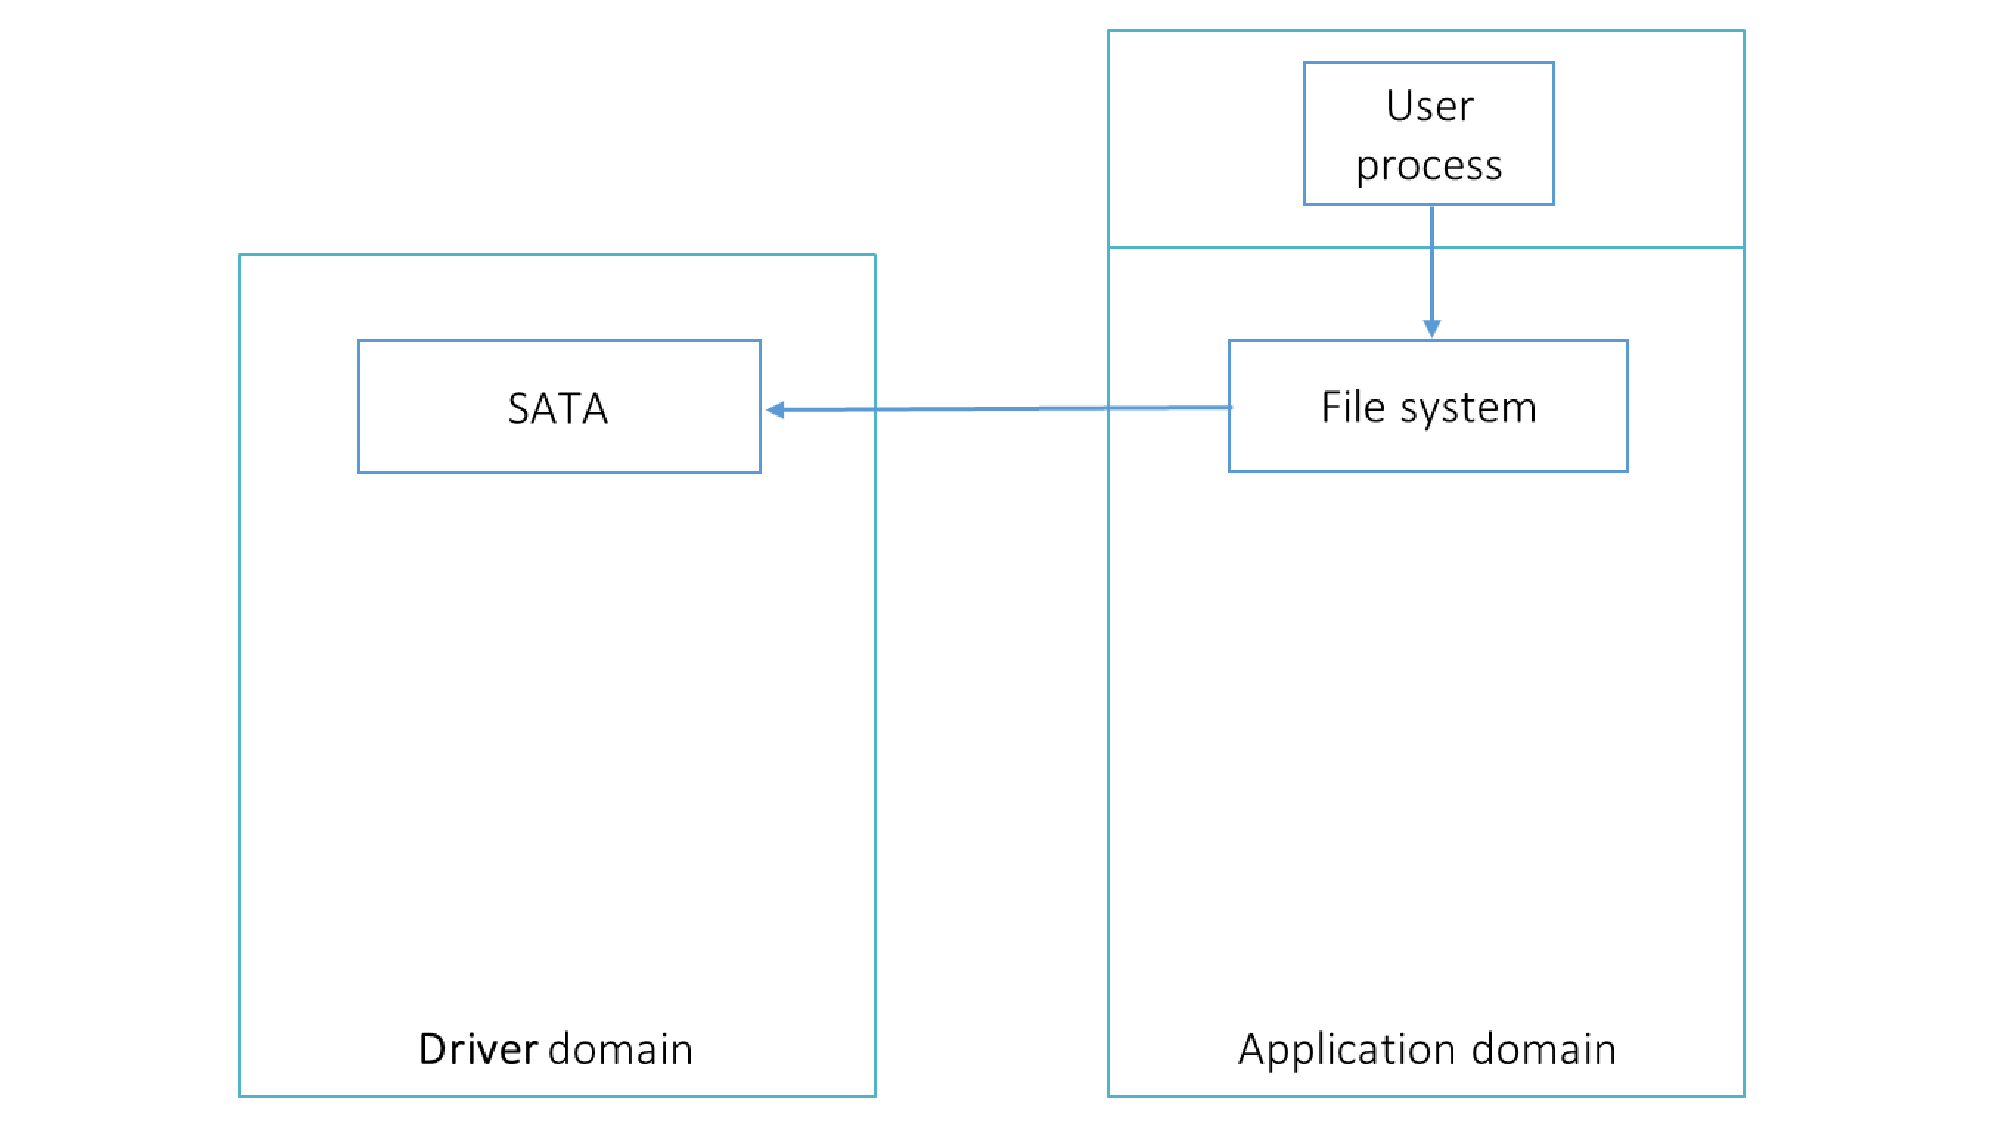
\includegraphics[scale=.25]{component1}
	\caption{Conceptual design of the driver domain}
	\label{fig:conept}
    \end{subfigure}
	\hfill
    \begin{subfigure}[b]{0.45\textwidth}
	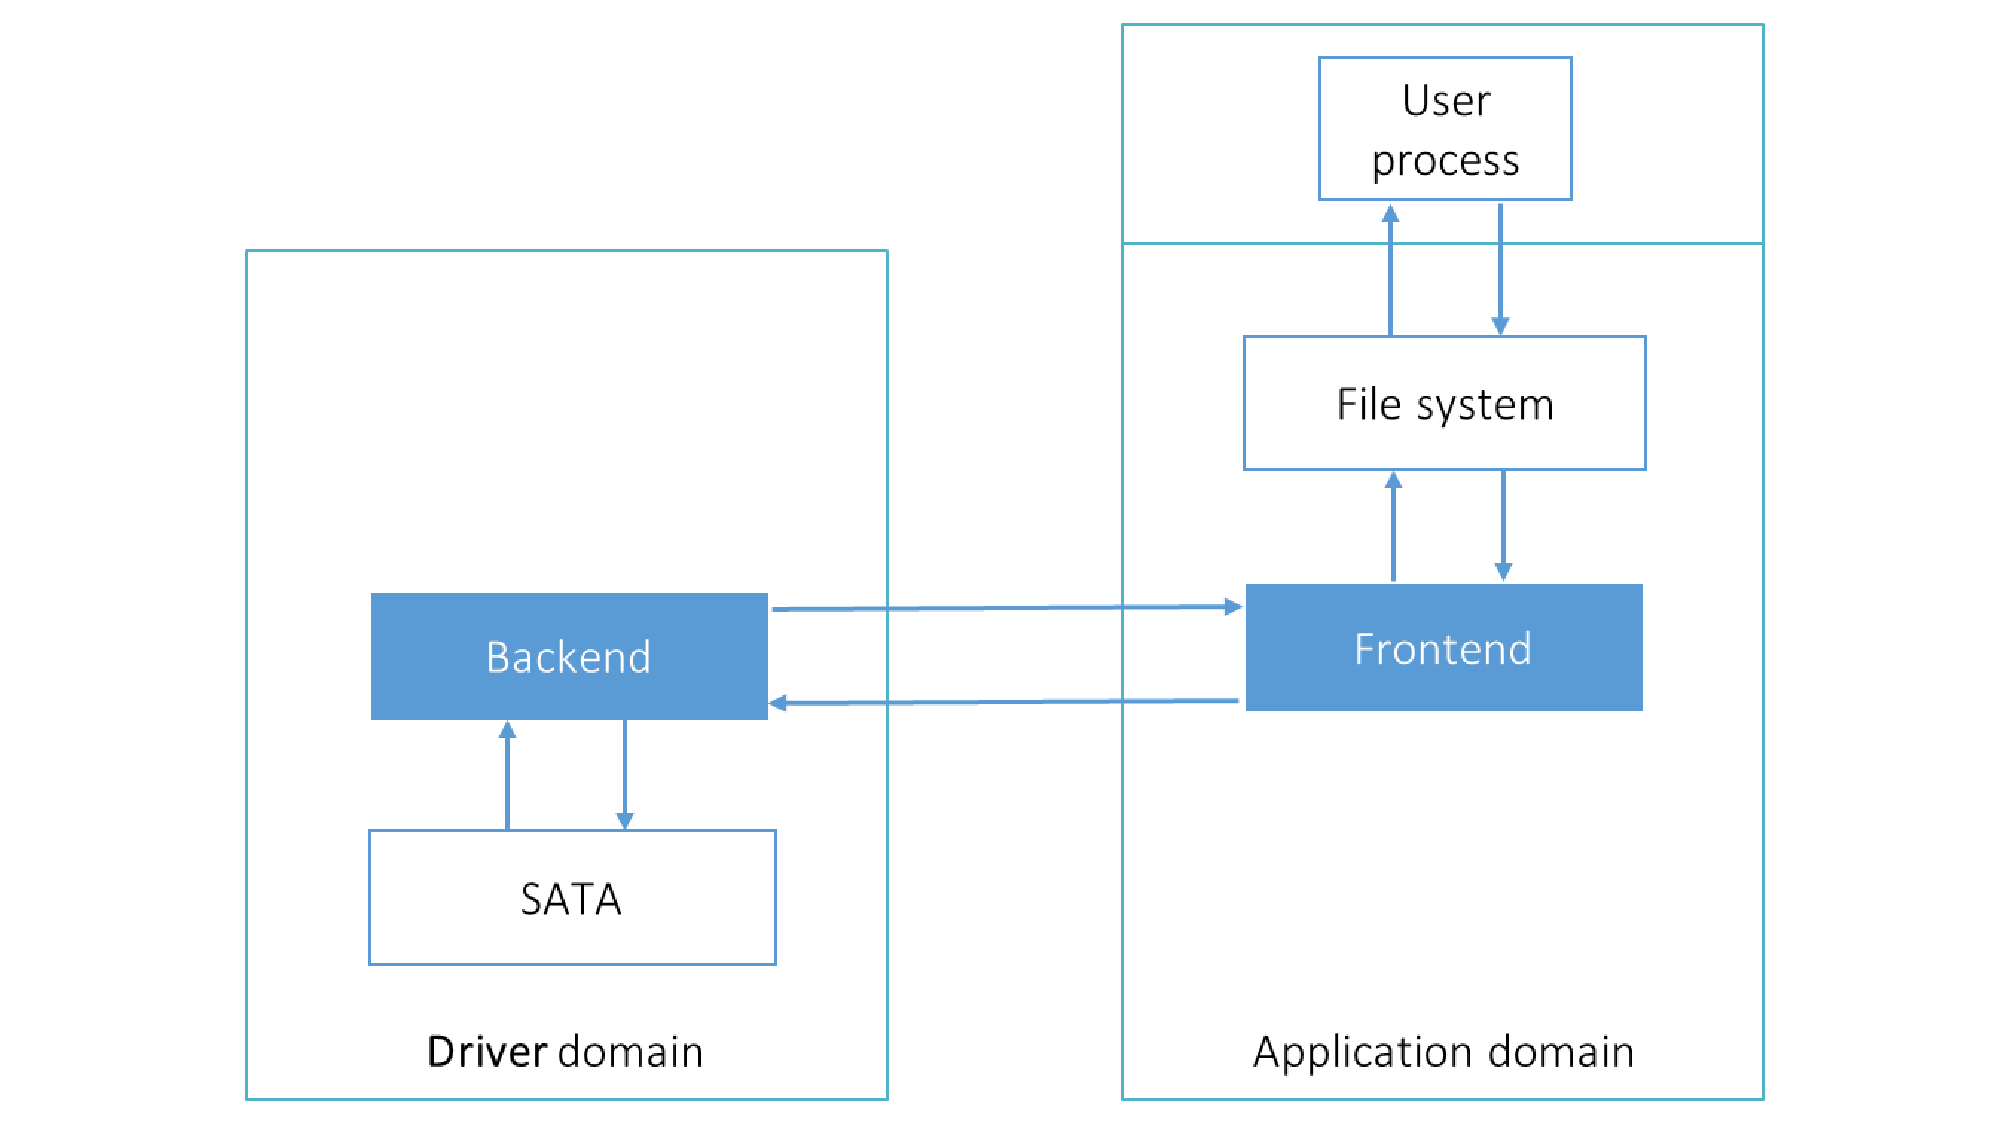
\includegraphics[scale=.25]{component2}
	\caption{Backend and frontend driver}
	\label{fig:backendfrontend}
    \end{subfigure}
    \caption{Role of frontend and backend driver}\label{fig:fault tolerence}
\end{figure}

\subsection{Communication module}
\label{sub:communicationmodule}
The communication module is the communication channel between the \textit{frontend driver} and the \textit{backend driver}. Unlike the \textit{backend driver} and the \textit{frontend driver}, the communication module is not a separate physical entity or a kernel module. It exists in the \textit{frontend driver} and the \textit{backend driver}. The communication channel is logically divided into three parts. 
\begin{enumerate} 
\item The responsibility of the first part is to share the requests and responses between the driver domain and the application domain.
\item The responsibility of the second part is to share the data of read/write requests/responses.
\item The responsibility of the third part is to notify the domain upon the occurrence of a particular event. 
\end{enumerate}

Figure~\ref{fig:communication} illustrates the role of the communication model. 
\begin{figure}[!ht]
\centering
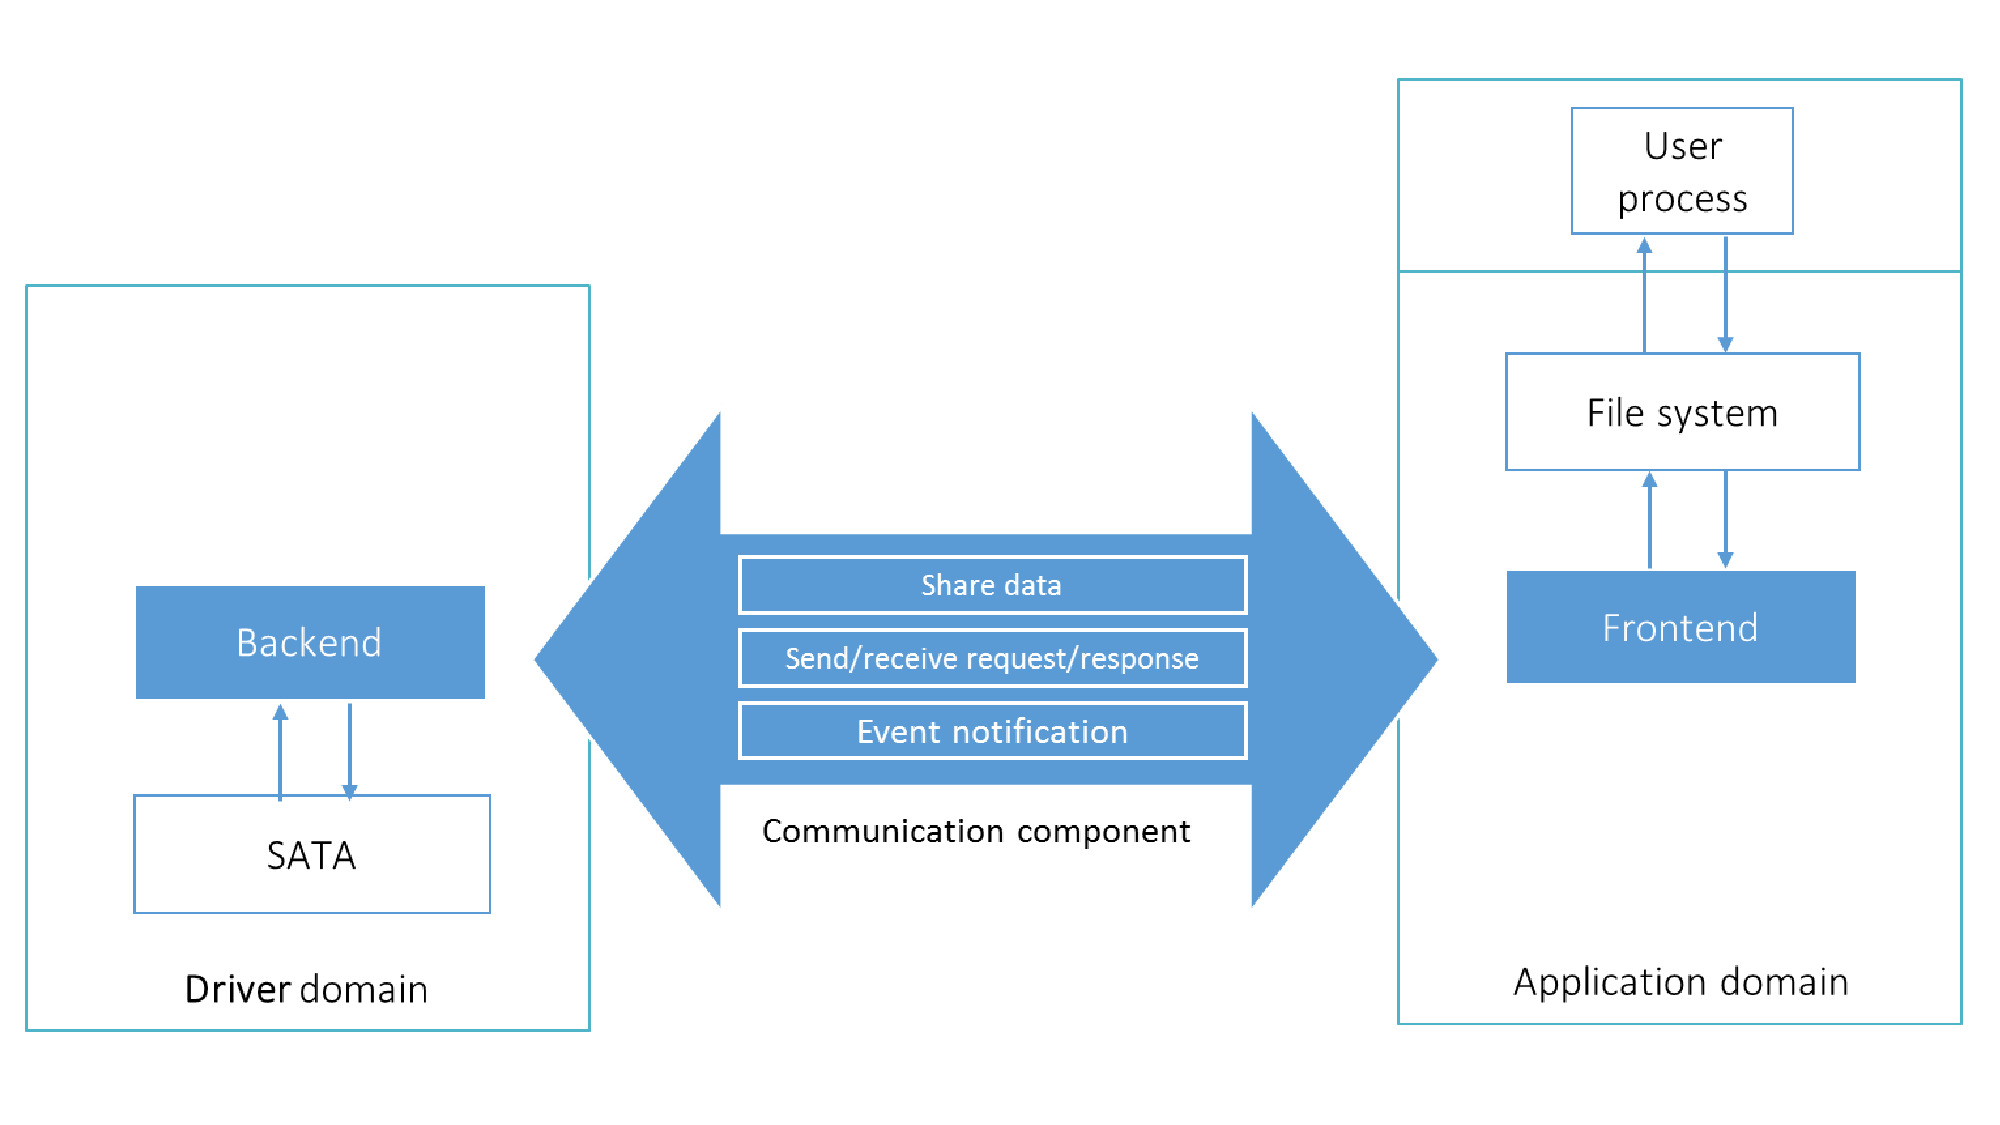
\includegraphics[scale=.5]{communicationmodule}
\caption{Communication module}
\label{fig:communication}
\end{figure}

\section{System design}\label{design}

The following section describes the design of the base IDDR system and the new IDDR system. 

\subsection{Communication module}

\paragraph{Base IDDR system design}
\label{par:base IDDR communication}
In the base IDDR system, the frontend driver submits requests to the communication channel. The communication channel copies data of the write requests in a shared memory. The communication module is responsible for the allocation and de-allocation of the shared memory. Once the sufficient number of requests are submitted by the frontend driver, the communication channel shares the requests with the backend driver. It notifies the backend driver that requests are available in a shared request queue.

\paragraph{Spinlock based IDDR system}
\label{par:spin IDDR communication}
As the Section~\ref{par:base IDDR communication} describes, in the base IDDR system, the communication module notifies the backend about the avaiability of the reqesuts in the shared queue. A software interrupt is sent to the domain as a notification. Each software interrupt which is sent for the availability of requests, causes the hypervisor to schedule the driver domain. Similarly, a software interrupt which notifies the availability of responses causes the hypervisor to schedule the application domain. The scheduling of the driver domain and the application domain might result in a context swtich. 
\\[3mm]
In order to avoid the context switch, we run an intermediate thread in the frontend driver and an intermediate thread in the backend driver. These both threads spin for the availability of requests and responses in the shared queue. The intermediate threads delegrates the responsibility of the notifications from the communication module to the frontend driver and backend driver. 

\subsection{Frontend driver}
\paragraph{base IDDR system design}
In the IDDR system, the frontend driver provides an interface to accept the requests from user application on behalf of the device driver. As explained in the Section~\ref{subsec:request queue}, each block device driver has a separate request queue to accept the the requests from user applications. Similar to the block device drivers, the frontend driver also creates a per device request queue to accept requests from user applications. If the sufficient requests are received, the frontend driver flushes the requests to the communication channel. The frontend driver receives a software interrupt upon availability of the responses in the shared queue. The frontend driver handles the software interrupt by reading data from the shared memory and ending the request in case of a read operation, otherwise it ends the requests without accessing the shared memory.

\paragraph{Spinlock based IDDR system}
As explained in the Section~\ref{par:spin IDDR communication}, we introduce an intermediate thread to read responses from the shared queue. The intermediate thread spins for responses. Upon availability of a response, the thread reads the response ends the corresponding request. If the corresponding request is a read request then the thread reads the shared data too. However, there still exists an intra-domain context switch between frontend driver main thread and the intermediate thread. The main thread is responsible for reading the requests from the frontend driver request queue (per device request queue), and flushing them to the communication channel. The main thread context switches to the intermediate thread, which spins for the responses. 
\\[3mm]
To avoid the intra-domain context switch, we introduce a spinlock in the frontend driver. In frontend driver, the main thread spins for the responses for a short time. If a response is available then similar to intermediate thread, the main thread reads the response and shared data and ends the corresponding request. However, in case of unavailability of a response, the main thread proceeds to read the new requests from the frontend driver request queue and the intermediate thread checks for the responses.  

\subsection{Backend driver}
\paragraph{Base IDDR system design}
in the base IDDR system, the backend driver receives a software interrupt from the frontend driver. In the software interrupt handler, the backend driver for the request to the device driver. Upon completion of the requests, the backend driver reads the response and puts it in shared queue. It also copies the read operation data to the shared memory. 

\paragraph{Spinlock based IDDR system}
As explained in the Section~\ref{par:spin IDDR communication}, we introduce an intermediate thread to read the request from the shared memory. The intermediate thread spins for the requests and upon availability of a request, it forwards the request to the device driver for the execution. The backend driver reads the response from the device driver and shares it in shared queue.
\begin{figure}[!ht]
\centering
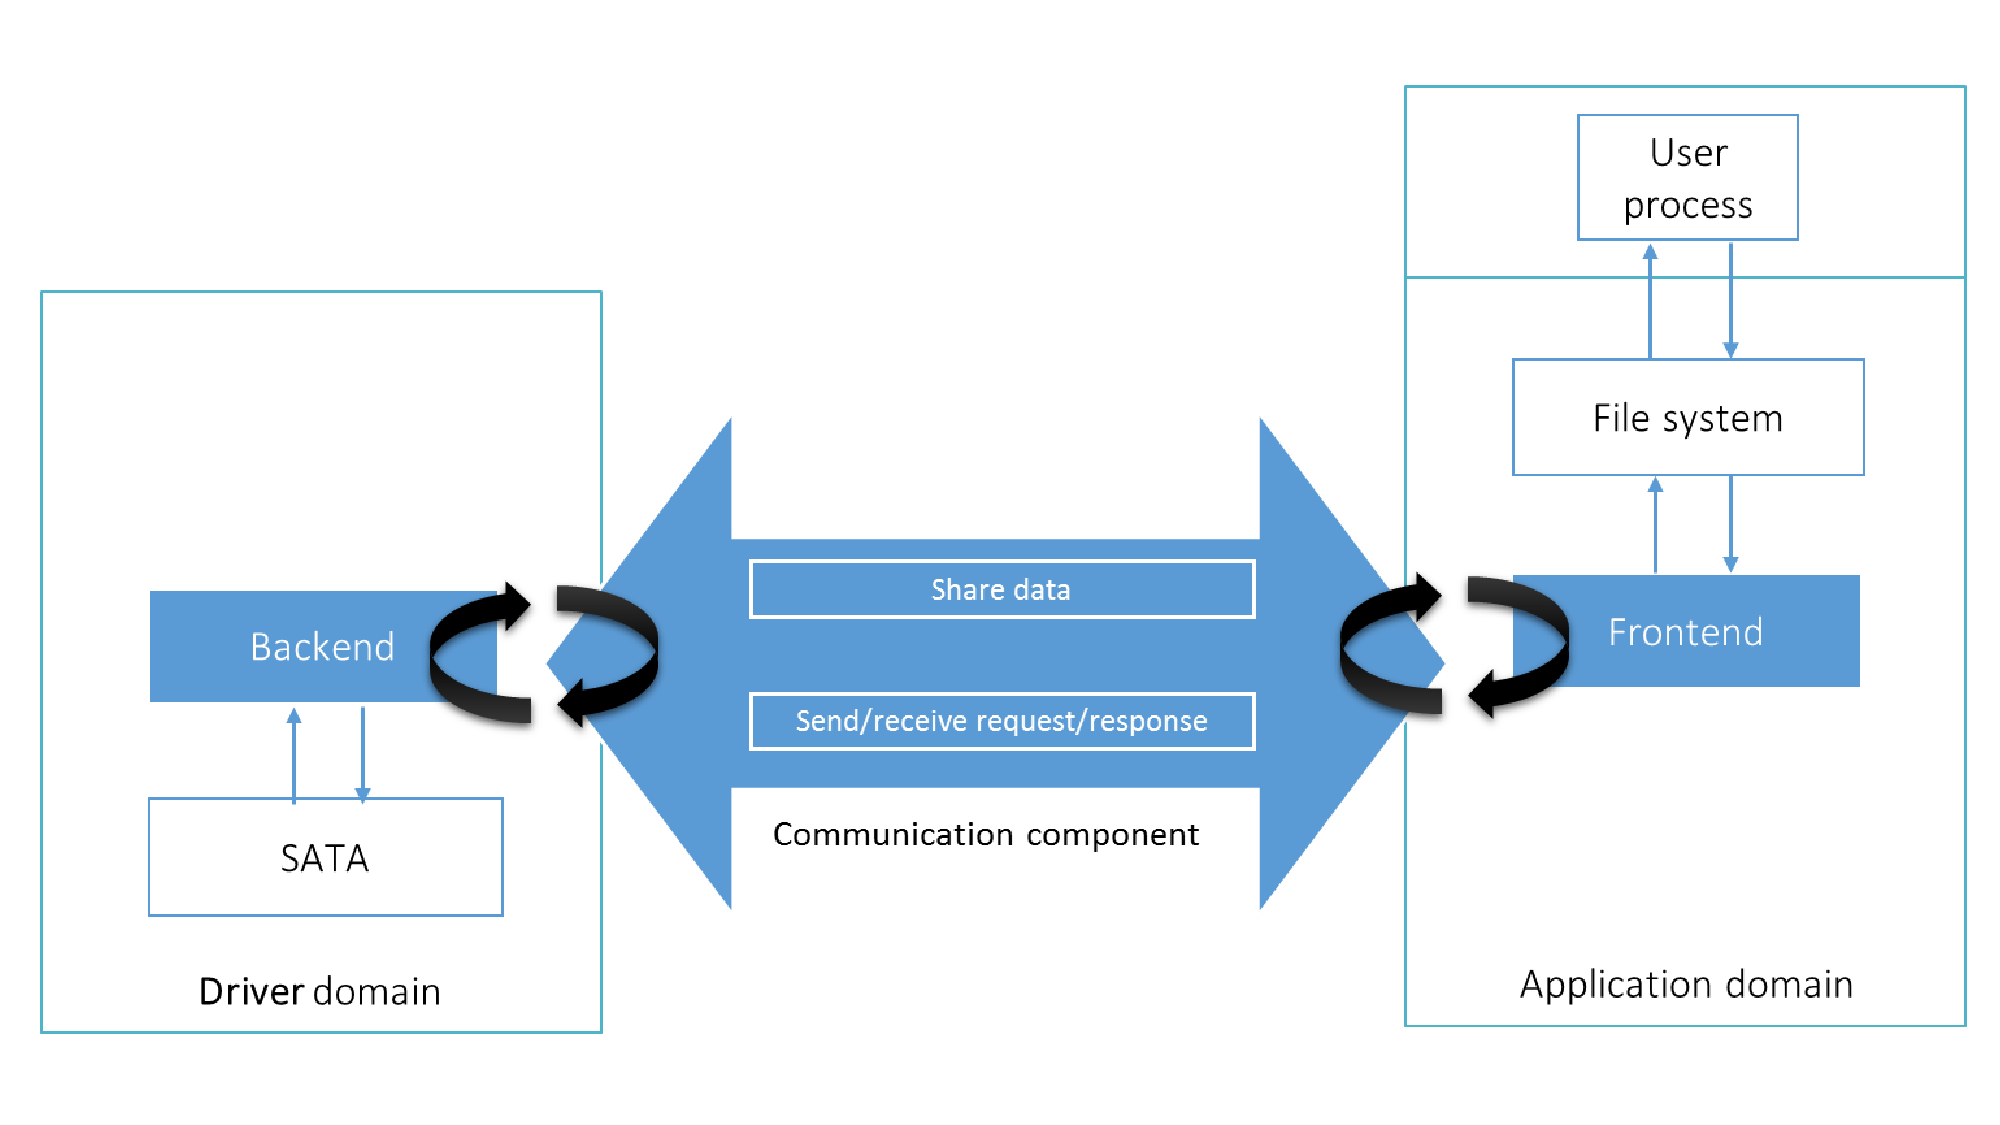
\includegraphics[scale=.5]{IDDRdesign}
\caption{Spinlock based new IDDR system}
\label{fig:new IDDR system}
\end{figure}

% \section{fault tolerance}
% Figure~\ref{fig:driver crash} and Figure~\ref{fig:high avail} explains the effects of a malicious activity occurring in the device driver isolated from the Linux kernel. When a device driver running in a driver domain hits a bug, it crashes the kernel of the driver domain and hence the driver domain itself. In addition, applications expecting a response from the driver domain might hang or crash waiting for the response. But due to the address space separation of the application domain and the driver domain, the application domain will remain intact.   
% \begin{figure}[!ht]
%     \centering
%     \begin{subfigure}[b]{0.45\textwidth}
% 	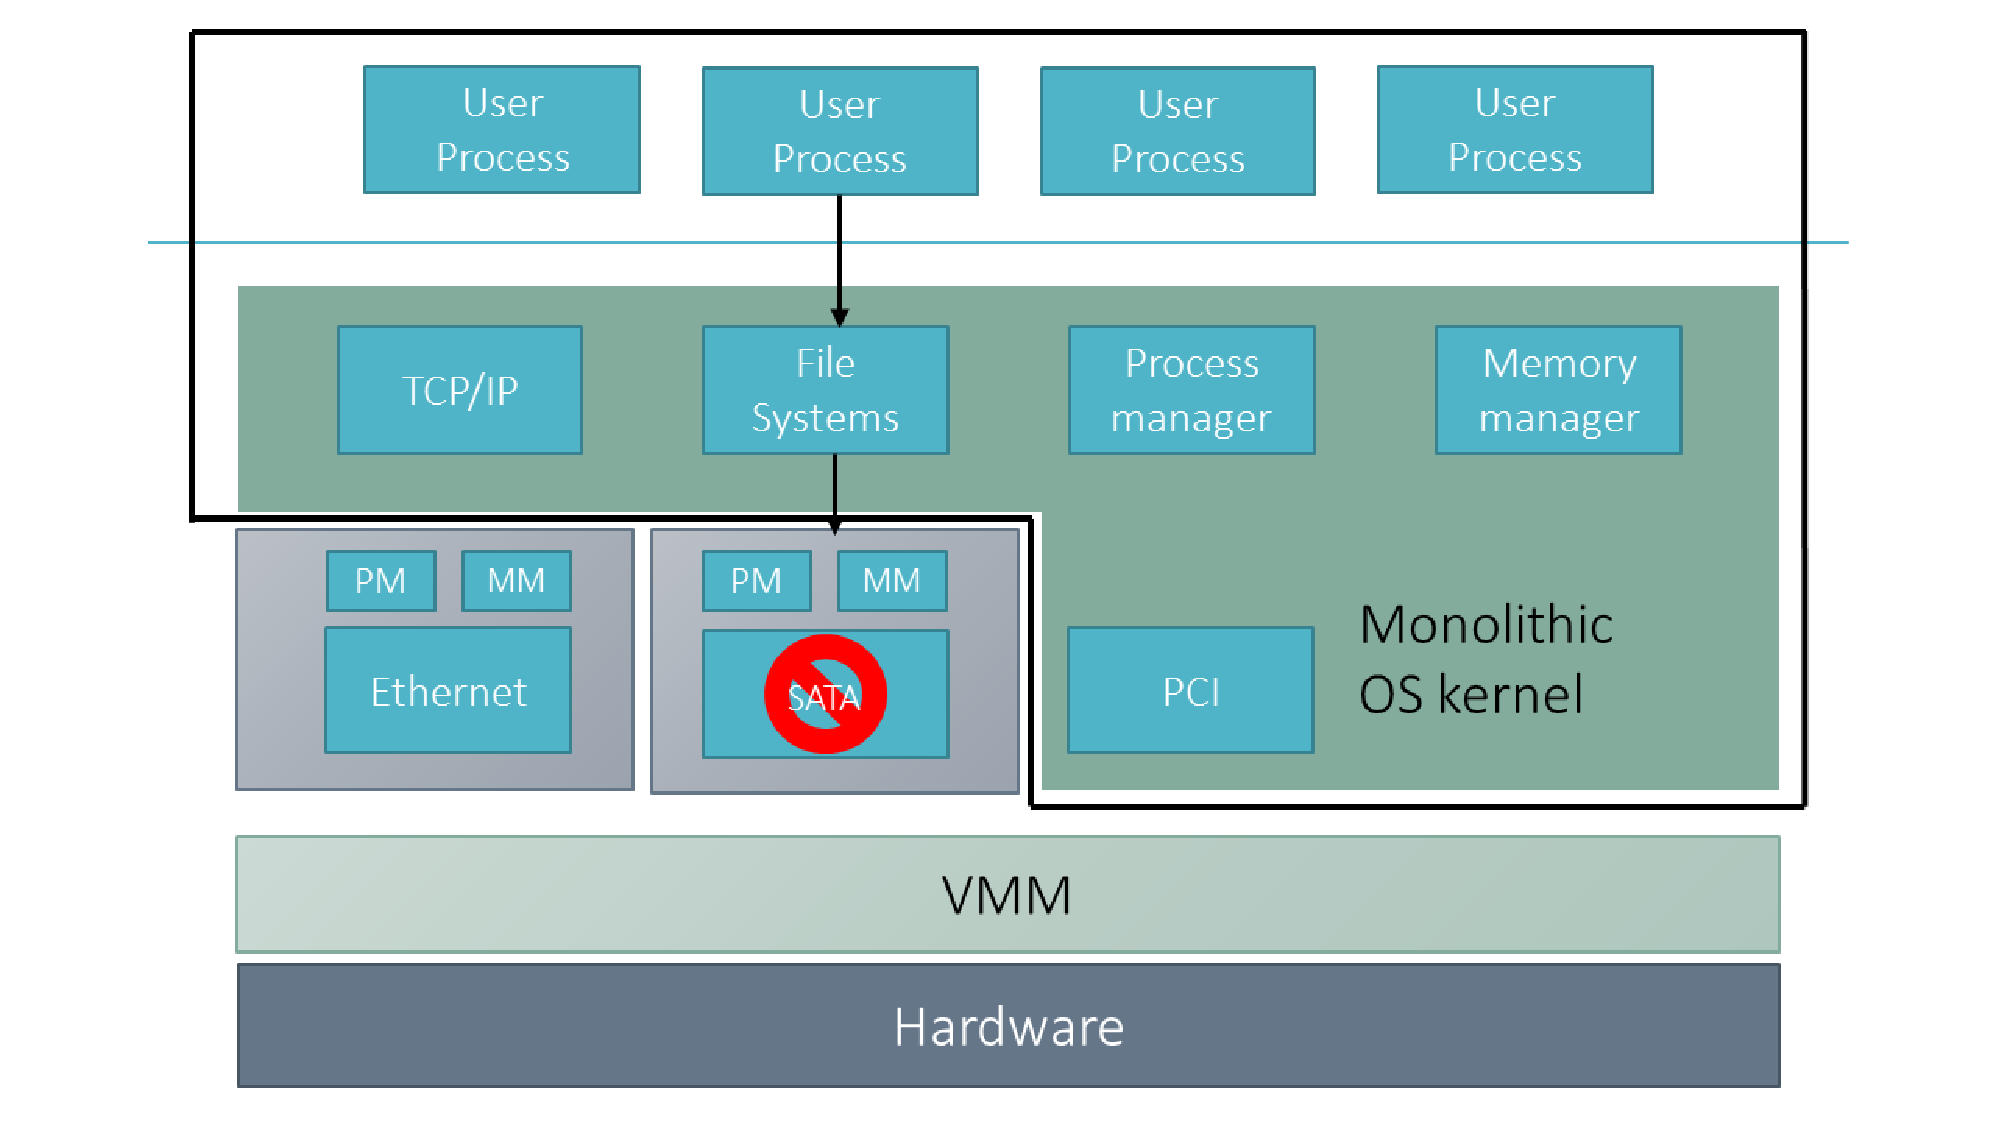
\includegraphics[scale=.25]{IDDRcrash1}
% 	\caption{Device driver crash}
% 	\label{fig:driver crash}
%     \end{subfigure}
% 	\hfill
%     \begin{subfigure}[b]{0.45\textwidth}
% 	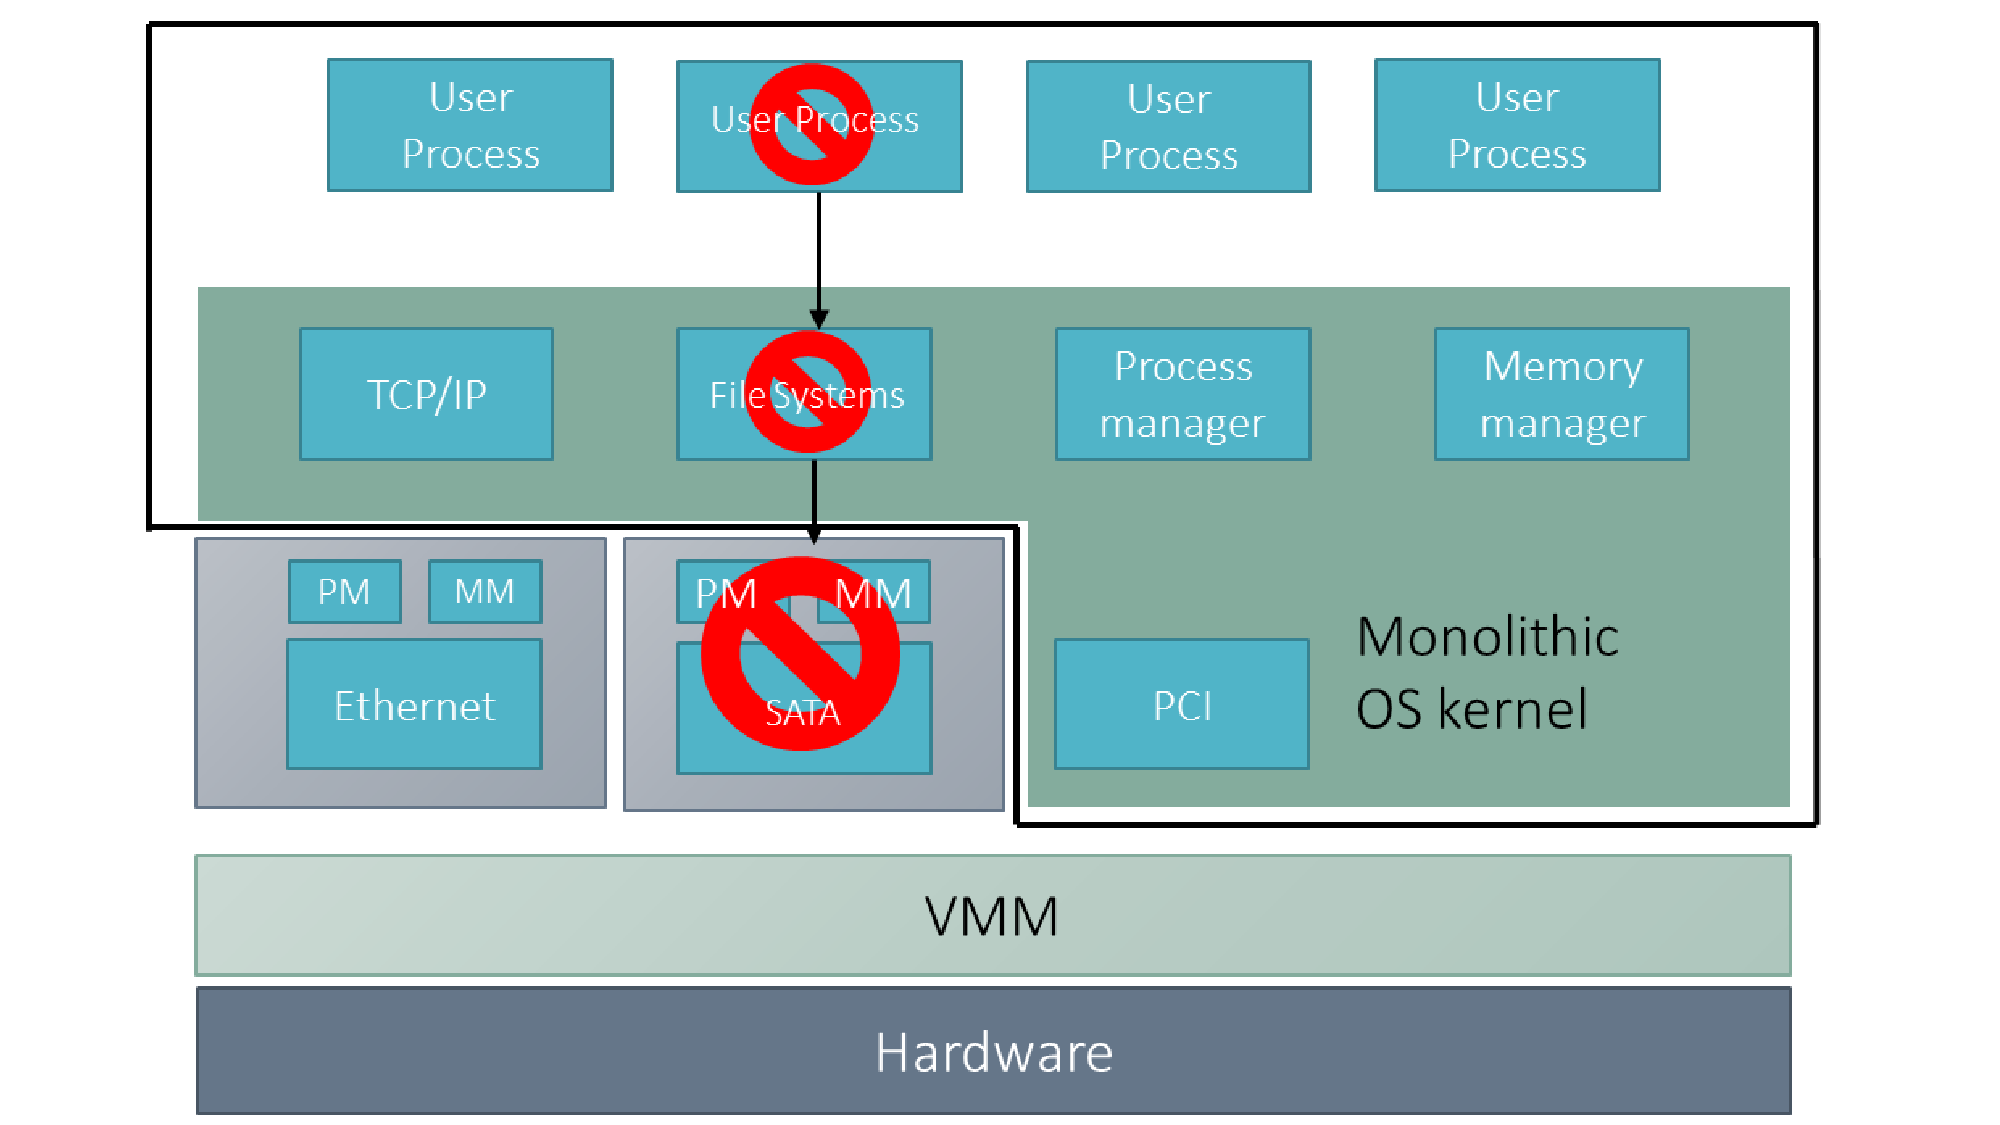
\includegraphics[scale=.25]{IDDRcrash2}
% 	\caption{Intact system}
% 	\label{fig:high avail}
%     \end{subfigure}
%     \caption{Fault tolerence}\label{fig:fault tolerence}
% \end{figure}
    
\ifbool{toShowBibliography}{\bibliography{references}}{}


\chapter{Implementation}
\markright{Sushrut Shirole \hfill Chapter 4. System Design and Implementation \hfill}

This chapter describes specific implementation details of IDDR system.

\section{Overview} 
We implemented the IDDR system based on the Linux kernel, version 3.5.0 and
Xen version 4.2.1. The application domain and the driver domain run the same kernel
binary. Table~\ref{tab:base} summarizes our implementation efforts in
terms of the number of lines of code.

\begin{table}
\caption{Implementation efforts in terms of number of lines of code.}
\begin{center}
\begin{tabular}{lll}
  \hline
  \label{tab:base}
  Component & Interrupt based IDDR & Spinning based IDDR \\
  \hline
  Linux Kernel & 6 & 6\\
  Xen & 252 & 252\\
  Front-end Driver & 611 & 712\\
  Back-end Driver & 692 & 752\\
  \hline 
  Total & 1561 & 1722\\
  \hline
\end{tabular}
\end{center}
\end{table}

The IDDR system implementation did not require any changes to the device
driver code. However, we did make a small number of changes to the Xen
and Linux kernel.

Figure~\ref{fig:Implementation overview} shows the implementation overview of 
the spinning based IDDR system.

\begin{figure}[!ht]
\centering
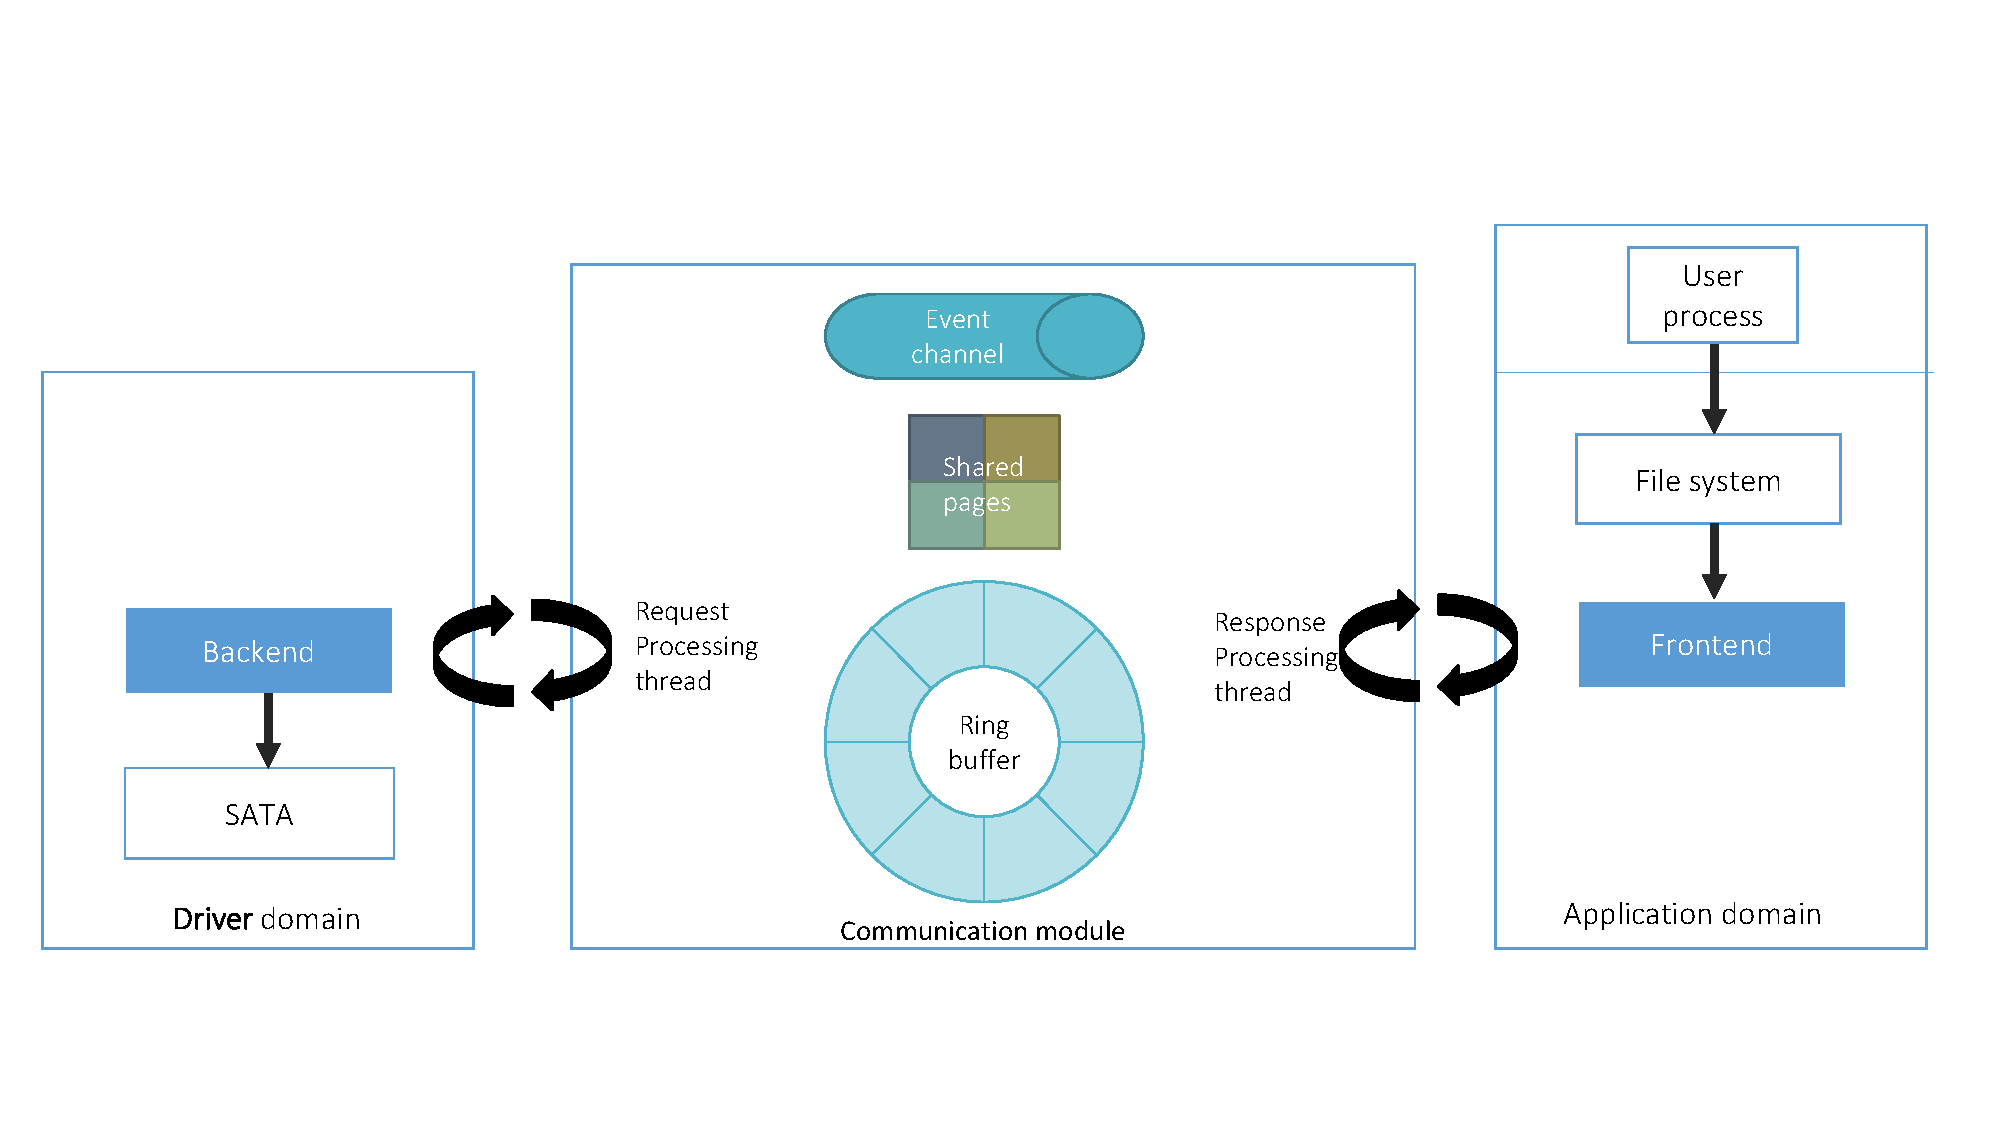
\includegraphics[scale=.5]{impl_overview_new}
\caption{Implementation overview of spinning based IDDR system}
\label{fig:Implementation overview}
\end{figure}

\section{Communication Module}
This section describes the implementation details of the communication
module of interrupt based IDDR system and spinning based IDDR system.

\subsection*{Interrupt based IDDR system}
As Section~\ref{sub:communicationmodule} describes, the role of the communication module in interrupt based IDDR system is to:
\begin{enumerate} 
\item Share requests and responses between the driver domain and the application domain
\item Share the data associated with read/write requests/responses
\item Notify the domain upon the availability of requests and responses 
\end{enumerate}
\paragraph{Shared Request and Response Queue:}
In order to implement the first role of the communication module, we
use the ring buffer mechanism provided by Xen. A ring buffer is a shared
I/O ring, which is explained in Section~\ref{subsec:io rings}. We divide
the ring buffer into the front ring and the back ring. The IDDR system
uses the front ring as the shared request queue and the back ring as
the shared response queue. The front ring shares requests and is called
as \textit{shared request queue}. The back ring shares responses and is
called as \textit{shared response queue}.

The IDDR system allocates the ring buffer in the initialization stage
of the communication module and initializes the ring buffer in the
application domain. Whenever the frontend driver receives a request from
an application in the application domain, the frontend driver removes the
request from the device driver queue and submits it to the communication
module. The communication module checks for a free space in the shared
request queue, and if available, it allocates the space for the new
request. After batching requests together, the communication module
pushes all requests to the shared request queue.

\paragraph{Shared Memory for Read/Write Data:}
We use the ring buffer only to share requests and responses. In order
to share data associated with read/write requests/responses we use
shared pages.

As explained in Section~\ref{subsec:sharedpages}, a grant table is used
for sharing memory between domains. We use a grant table to share memory
between the application domain and the driver domain.

\paragraph{Event Notification:}
We create a new event channel in the initialization stage of the
communication module in the application domain and connect to the same
event channel in the initialization stage of the communication module
in the driver domain. We attach an interrupt handle routine for the
event channel in both the application and driver domain. The interrupt
handler routine in the application domain reads responses from the shared
response queue and forwards them to the frontend driver. The interrupt
handler routine in the driver domain reads requests from the shared
request queue and forwards them to the backend driver.

\subsection*{Spinning Based IDDR System}
This section describes the communication module in 3 parts:

\paragraph{Shared Request and Response Queue:}
Similar to the interrupt based IDDR system, the communication module
uses a ring buffer as the shared request and response queue.

\paragraph{Shared Memory for Read/Write Data:}
Similar to interrupt based IDDR system, the communication module uses a
grant table to share an allocated memory between the application domain
and the driver domain.

\paragraph{Threads and Event Notification:}
In order to improve the performance of the IDDR system, we implement the
communication module where a thread in the frontend driver spins for the
availability of responses, and a thread in the backend driver spins for
the availability of requests. In case of unavailability of requests and
responses, both threads go to sleep.

The spinning based IDDR system uses an event channel to wake the read
request thread sleeping in the application domain. The wake up signal
is sent in the form of an event channel notification from the driver
domain to the application domain. Similarly, to wake the read response
thread sleeping in the driver domain, an event channel notification is
sent from the application domain to the driver domain.

\begin{itemize}
\item \textbf{Read response thread in the application domain:} 
In the spinning based IDDR system we create a kernel thread called the \textit{read
response thread} during an initialization stage of the communication
module in the application domain. The \textit{read response thread} spins
to check if responses are available in the shared response queue. If a
response is available, it reads the response from the shared response
queue. However, if a response is not available in the shared response
queue, after spinning for some time the thread goes into a sleep state. We
maintain the status of the thread as \texttt{SLEEPING} or \texttt{RUNNING}
in the shared data structure. We use an atomic variable to save the
state of the thread, avoiding race conditions.

Obviously, a thread shouldn't sleep unless it is assured that somebody else, somewhere, will wake it up. The code doing the waking up must also be able to identify the thread to be able to do its job. We use a Linux data structure called \texttt{wait queue} to find the sleeping thread. Wait queue is a list of threads, all waiting for a specific event\cite{Galvin, Bovet:2005:ULK:1077084}. We initialize the wait queue for the read response thread during an initialization stage of the communication module in the application domain. The read response thread sleeps in the wait queue, waiting for a flag denoting the availability of the response to be set. The communication module in the driver domain checks the status of the read response thread after pushing responses on the shared response queue. If the status is \texttt{SLEEPING} then it sends a software interrupt through the event channel.

Similar to interrupt based IDDR system, we create a new event channel in
the initialization stage of the communication module in the application
domain. We attach an interrupt handler routine for the event channel
in the application domain. In the interrupt handler, the communication
module wakes up the read response thread if it is sleeping.

\item \textbf{Read request thread in the driver domain:}
In spinning based IDDR system, we create a kernel thread during
an initialization stage of the communication module in the driver
domain. This new kernel thread is called the \textit{read request
thread}. The \textit{read request thread} spins to check if requests are
available in the shared request queue. If a request is available, it reads
the request from the shared request queue. However, if a request is not
available in the shared request queue, the thread goes into a sleep state
after spinning for some time (adaptive spinning). Similar to the read
response thread, we maintain the status of the thread as \texttt{SLEEPING}
or \texttt{RUNNING} as a atomic variable in the shared data structure.

We initialize a wait queue for the read request thread during
an initialization stage of the communication module in the driver
domain. The read request thread sleeps in the wait queue, waiting for a
flag denoting availability of the request to be set. The communication
module in the application domain checks the status of the read request
thread after pushing requests on the shared request queue. If the status
is \texttt{SLEEPING} then it sends a software interrupt through the
event channel.

Similar to interrupt based IDDR system, the driver domain connects to the
event channel created by the application domain in the initialization
stage of the communication module. We attach an interrupt handler
routine for the event channel in the application domain. In the interrupt
handler, the communication module wakes up the read request thread if
it is sleeping.  
\end{itemize}

\section{Application Domain}

Application domain is the domain running user applications and the Linux
kernel. In a Linux system, usually a user process sends the read write
request to a file system, which sends the read and write request to
the block device driver. The block device driver serves the request and
sends back a response to the file system, which then sends the response
to the user process.

In the IDDR system implementation, a block device runs separately in
the driver domain. When a user process sends a request to a file system,
the file system needs to forward the request to the driver domain. Like
explained in Section~\ref{subsec:frontend}, in the IDDR system, a piece
of code called the frontend driver forwards the request to the driver
domain running the block device driver.

\subsection*{Interrupt based IDDR System}
The core responsibility of the frontend driver in interrupt based IDDR system is to:
\begin{enumerate}
\item Provide an interface which appears as a block device to the upper layer in the stack
\item Accept a request from the upper layer
\item Create a corresponding new request which can be understood by the driver domain
\item End the request after reading the response
\end{enumerate}

Implementation details of the frontend driver can be split into 3 stages: 
\begin{enumerate}
\item Initialization
\item Submit request to the communication module
\item End request
\end{enumerate}

\paragraph{Initialization}
During the initialization, the frontend driver creates a separate
interface for each block device. The interface for each block device is
associated with a device driver queue. Read and write requests issued
on the interface get queued in this device driver queue.

\paragraph{Dequeue and Submit Request:}
The frontend driver removes the request submitted to the driver
interface and converts the request into a request structure, which is
understood by the backend driver. The new request structure points to
the shared memory allocated for the read/write data by the communication
module. The frontend driver then forwards the newly created request
to the communication module, which also shares the request with the
backend driver.

\paragraph{End Request:}
We maintain a shadow table of all requests which were received in the
device driver queue. The shadow table is a table which contains an entry
of all the requests received. We implement the shadow table as a circular
array of the requests. We maintain an ID for each request. The backend
driver copies this ID into the corresponding response. The ID is used
for mapping the response to the request in the shadow table. When a
response is read by the communication module, it forwards the response
to the frontend driver. The frontend driver searches the corresponding
request in the shadow table, and ends it.

\subsection*{Spinning Based IDDR System}
The core responsibility of the frontend driver in spinning based IDDR system is to:
\begin{enumerate}
\item Provide an interface for each block device
\item Accept a request from the upper layer
\item Create a corresponding new request which can be understood by the driver domain
\item Spin for a short time while waiting for the response
\item End the request
\end{enumerate}

Implementation details of the frontend driver is split into 4 stages:
\begin{enumerate}
\item Initialization
\item Submit request to the communication module
\end{enumerate}

\paragraph{Initialization:}
Similar to interrupt based IDDR system, during the initialization process the frontend driver creates an interface for each block device.

\paragraph{Dequeue and Submit Request:}
Similar to interrupt based IDDR system, the frontend driver removes the
request submitted to the driver interface and converts it into the request
structure with a data pointer pointing to the shared memory. The frontend
driver then forwards the newly created request to the communication
module, which also shares the request with the backend driver.

\section{Driver Domain}
The IDDR system runs a block device driver in the driver domain. Like
explained in Section~\ref{subsec:backend}, a piece of code called the
backend driver runs in the driver domain, which accepts requests from
the application domain and forwards requests to the device driver. Upon
receiving a response from the device driver, the backend driver sends
back the response to the communication module.

\subsection*{Backend Driver}
The role of the backend driver in the IDDR system is to:
\begin{enumerate}
\item Read a request through the communication module and convert it to a bio request
\item Accept a response from the block device driver
\item Forward the response to the communication module
\end{enumerate}

Implementation details of the backend driver can be split into 2 stages. 
\begin{enumerate}
\item Convert a request to the bio request. 
\item Make a response.
\end{enumerate}

\subsubsection*{Convert a Request to Bio}
\label{subsec:createbio}
The backend driver converts a request that is shared through the
communication module into a bio request, so that the block device
understands the request. In order to make the bio request, pages from
the shared memory are mapped and inserted into the bio structure and
required information is copied from the shared request into the bio
structure. At the end, the newly created bio request is sent to the
lower layer for execution. Once the bio request execution is completed,
the system calls a callback function.

\subsubsection*{Make a Response and Enqueue}
Irrespective of the success or failure of execution of a bio request,
the backend driver makes a response in the callback function. In this
callback function, the result of the bio execution and a request ID is
copied into a newly allocated response structure. The request ID is used
as an index in the shadow table to map a response and a request. The
communication module pushes the response into the shared response queue.



\chapter{Evaluation}
\markright{Sushrut Shirole \hfill Chapter 6. Evaluation \hfill}

We use \texttt{Linux kernel 3.5.0} for both application domain and driver domains. We use the Arch Linux distribution for the \texttt{x86\_64} platform for our testing and performance evaluation. The specifications of the system used for the evaluation is presented in Table~\ref{tab:config}. 

\begin{table}
\caption{Hardware specifications}
\begin{center}
\begin{tabular}{ll}
  \hline
  \label{tab:config}
  System Parameter & Configuration \\
  \hline
  Processor & 2 X Quad-core AMD Opteron(tm) Processor 2380, 2.49 Ghz \\
  Number of cores & 4 per processor \\
  Hyperthreading & OFF \\
  L1 L2 cache & 64K/512K per core \\
  L3 cache & 6144K \\
  Main memory & 16Gb \\
  Storage & SATA, HDD 7200RPM \\
  \hline 
\end{tabular}
\end{center}
\end{table}

\section{Goals}
\label{sec:goals}
The goals of our evaluation are:
\begin{enumerate}
\item \textbf{Comparison  of Xen's isolated driver domain with the interrupt based IDDR system:}

In order to prove the performance improvement of the spinning based IDDR system over the interrupt based IDDR system and the Xen's isolated driver domain, it is necessary to compare the performance of the Xen's isolated driver domain with the interrupt based IDDR system. Since source code of the isolated driver domains is not available and it follows split device driver architecture, we achieve this evaluation goal by comparing the performance of the interrupt based IDDR system with Xen's split device driver.

\item \textbf{Performance impact of spinning-based optimization:}

The second goal of the evaluation is to prove that the spinning based communication channel improves the performance of the inter-domain communication and hence the IDDR system.

We achieve this evaluation goal by comparing the performance of the interrupt based IDDR system with the spinning based IDDR system.
\end{enumerate}

\section{Methodology}
\label{sec:methodology}
In order to measure the performance of the system, we run performance tests using a variety of block devices. In order to cover a variety of the devices we use block devices such as SATA disk, ramdisk and loop device for the performance testing. A loop device is a device that makes a file accessible as a block device. A ramdisk is a block of a memory, which acts as a disk drive. 

In order to conduct the performance tests, we format the block device with the ext2 file system, and run the fileIO SysBench benchmark~\cite{sysbench} on it. SysBench is a multi-threaded benchmark tool for evaluating a file system. SysBench benchmark has different test modes. FileIO is one of the test mode. FileIO can be used to produce different file I/O workloads. It runs a specified number of threads to execute requests in parallel. We run the SysBench benchmark in fileIO test mode to generate 128 files with \texttt{1Gb} of total data. We execute random reads, random writes, a mix of random reads and writes on all three devices. The block size was set to \texttt{16Kb}. We vary the number of SysBench threads from 1 to 32 to obtain the throughput of the system under different workload. 

\section{Xen Split Device Driver vs interrupt based IDDR System}
As per our first evaluation goal discussed in Section~\ref{sec:goals}, we compare the interrupt based IDDR with Xen's split device driver. 

\subsection*{Experimental Setup}

\subsubsection*{Xen Split Device Driver}
We create a ramdisk in domain 0. The guest domain (domain U) is configured such that the ramdisk uses a split device driver and is available in the guest domain. We do a similar setup for the loop device and the SATA disk. In the case of the loop device, we create a loop device in the domain 0 and then configure the guest domain to use the loop device as a disk. In case of SATA disk, we configure the guest domain such that the SATA disk uses split device driver. We format and mount the disk in the guest domain with the ext2 file system. The SysBench benchmark is run on the mounted partition as explained in section~\ref{sec:methodology}.

\subsubsection*{Interrupt Based IDDR System}
In Xen hypervisor, the domain 0 always runs as a paravirtualized guest and domain U can be a HVM guest or a PV guest. In our setup domain U always runs as a HVM guest. A HVM guest is expected to have less syscall overhead and faster memory bandwidth than a PV guest. We verified this behavior of PV and HVM guests by running syscall micro-benchmark of lmbench. We created a HVM domain U and ran syscall micro-benchmark in PV domain 0 and HVM domain U. We compared the result and came to conclusion that a PV guest has less syscall overhead than a HVM guest.

Since in Xen's split device driver runs the backend device driver in domain 0 and the frontend device driver in domain U, it is necessary to run the backend and frontend driver in domain 0 and domain U respectively in our system too.

We insert a ramdisk and the interrupt based IDDR system's backend module in domain 0 and the frontend module in the guest domain (domain U). We format and mount the ramdisk with ext2 file system and run the SysBench benchmark on it.  

A similar setup is used for a loop device. We create a loop device in domain 0 and insert the backend driver in the same domain. We insert the frontend module in the guest domain.

In order to use SATA disk in domain U we needed SATA controller of the disk to passthrough. However because of technical issues we couldn't passthrough SATA controller to domain U. Hence only for SATA disk experiment we use domain 0 as a driver domain and domain U as an application domain.

\subsubsection*{Comparison }
We compare the throughput of Xen's split device driver and the interrupt based IDDR system in Figure~\ref{fig:iddrvsxen-ramdisk-rdwr} and Figure~\ref{fig:iddrvsxen-loop-rd}. In this comparison Xen's split device driver is compared with IDDR system as a proxy for Xen's isolated driver domain. The Figure~\ref{fig:iddrvsxen-ramdisk-rdwr} presents the throughput of both systems when data is randomly read from a ramdisk and written to it. Figure~\ref{fig:iddrvsxen-loop-rd} presents the throughput when data is randomly read from a loop device. 
\\[3mm]
On a loop device, the performance of the interrupt based IDDR system differs by 3\%-4\% when compared to Xen's split device driver. On a ramdisk, the throughput of the interrupt based IDDR system matches that of the Xen split device driver. This proves that our implementation of the isolated driver domain provides a suitable baseline for our performance optimization.

\begin{figure}[!ht]
%\centering
  \begin{subfigure}[b]{0.2\textwidth}
  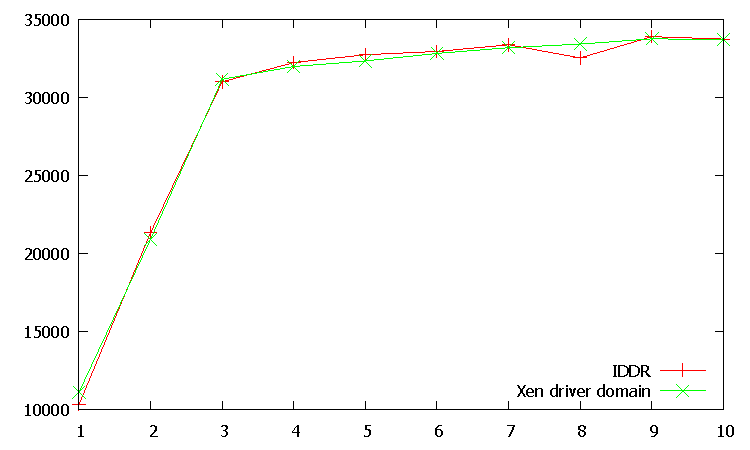
\includegraphics[scale=.7]{iddrvsxen-ramdisk-rdwr}
  \caption{Random reads-writes on a ramdisk}
  \label{fig:iddrvsxen-ramdisk-rdwr}
  \end{subfigure}
  \hspace{50mm}
  %\hfill
  \begin{subfigure}[b]{0.2\textwidth}
  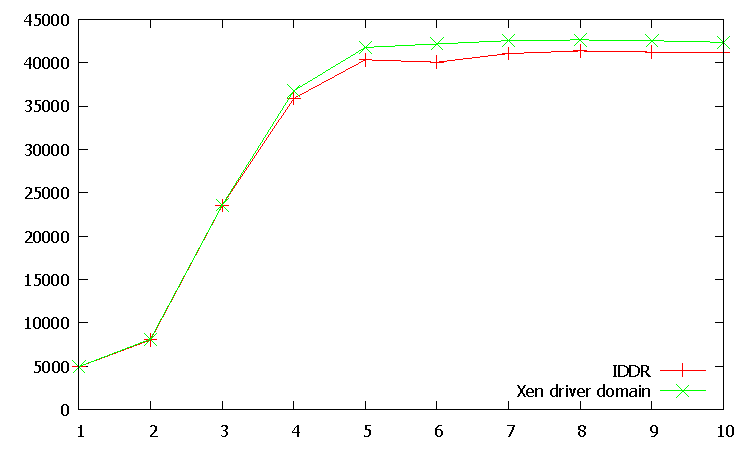
\includegraphics[scale=.7]{iddrvsxen-loop-rd}
  \caption{Random reads on a loop device}
  \label{fig:iddrvsxen-loop-rd}
  \end{subfigure}\\
\caption{Interrupt Based IDDR system vs Xen split driver}\label{fig:seqloopdisk}
\end{figure}

\section{Interrupt Based IDDR System vs Spinning Based IDDR System}
We measure and compare the performance of the interrupt based IDDR system with the spinning based IDDR system. To compare the performance of both systems, we measure performance of the system by varying the number of SysBench threads. The SysBench benchmark executes random read write on a ramdisk and loop device. 
\subsection*{Experimental Setup}
In both systems, the application domain is domain 0, and the driver domain is domain U. We create a ramdisk and insert the backend driver in the driver domain. We insert the frontend driver in the application domain. 

We measure the performance of both systems on a loop device with same setup.

\subsubsection*{Random reads and writes}

\paragraph{Comparison :}

Figure~\ref{fig:rndramdisk}, Figure~\ref{fig:rndloopdisk} and Figure~\ref{fig:rndharddisk} compares the throughput of the interrupt based IDDR and the spinning based IDDR system when data is randomly read from a ramdisk, loop device, SATA disk and is written on them.

Figure~\ref{subfig:rndrd-ramdisk}, Figure~\ref{subfig:rndrd-loopdisk} Figure~\ref{subfig:rndrd-harddisk} show that the spinning based IDDR system performs better when data is read from a device randomly.  

Figure~\ref{subfig:rndwr-ramdisk}, Figure~\ref{subfig:rndwr-loopdisk} and Figure~\ref{subfig:rndwr-harddisk} compare the performance of the device when data is written randomly to a device. The graph shows that initially the spinning based IDDR system performs better than the interrupt based IDDR system, but as number of SysBench threads increases, the throughput of the spinning based IDDR system decreases.
\\[3mm] 
Figure~\ref{subfig:rndrw-ramdisk}, Figure~\ref{subfig:rndrw-loopdisk} and Figure~\ref{subfig:rndrw-harddisk} compare the performance for mix random read and write workload. 

\begin{figure}[!ht]
% \centering
  \begin{subfigure}[b]{0.2\textwidth}
  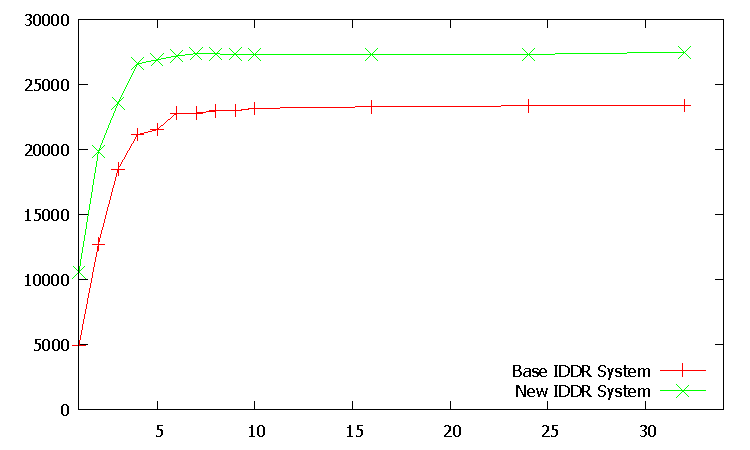
\includegraphics[scale=.7]{rndrd-ramdisk}
  \caption{Random reads}
  \label{subfig:rndrd-ramdisk}
  \end{subfigure}
  \hspace{50mm}
  \begin{subfigure}[b]{0.2\textwidth}
  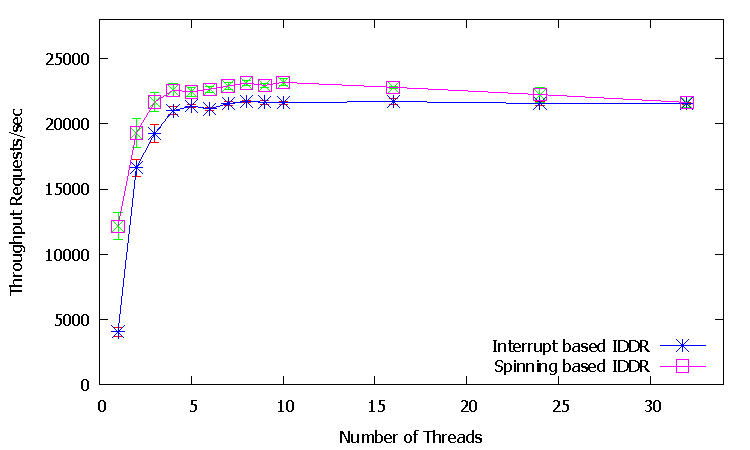
\includegraphics[scale=.7]{rndwr-ramdisk}
  \caption{Random writes}
  \label{subfig:rndwr-ramdisk}
  \end{subfigure}\\*
  \hspace{150mm}
  \begin{subfigure}[b]{0.3\textwidth}
  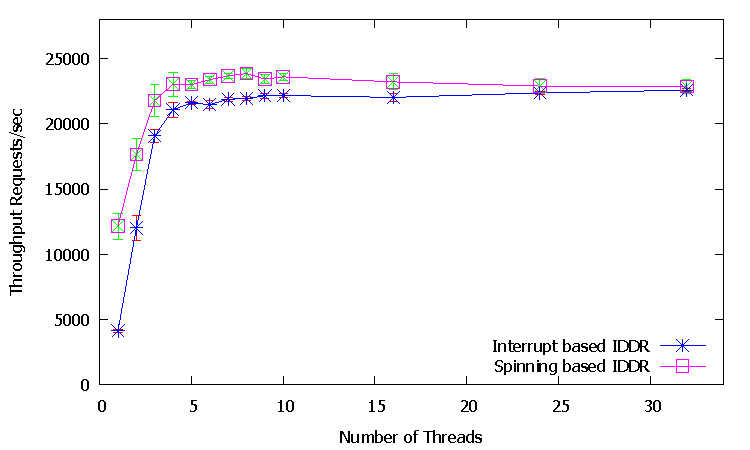
\includegraphics[scale=.7]{rndrw-ramdisk}
  \caption{Random reads writes}
  \label{subfig:rndrw-ramdisk}
  \end{subfigure}
  \caption{Random reads and writes on a Ramdisk}\label{fig:rndramdisk}
\end{figure}

\begin{figure}[!ht]
%\centering
  \begin{subfigure}[b]{0.2\textwidth}
  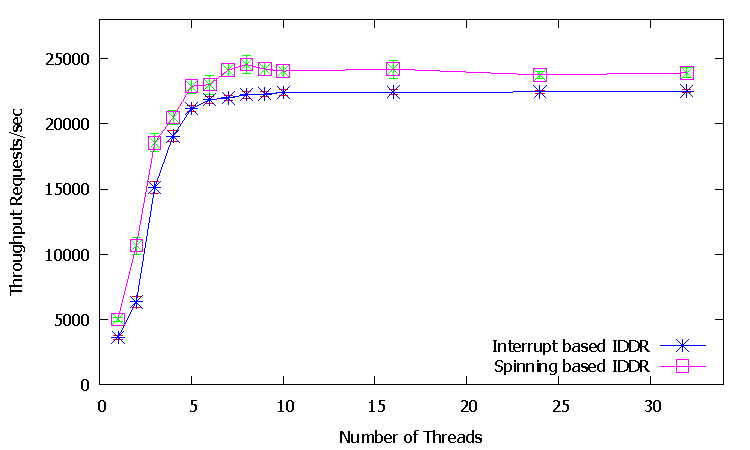
\includegraphics[scale=.7]{rndrd-loopdisk}
  \caption{Random reads}
  \label{subfig:rndrd-loopdisk}
  \end{subfigure}
  \hspace{50mm}
  \begin{subfigure}[b]{0.2\textwidth}
  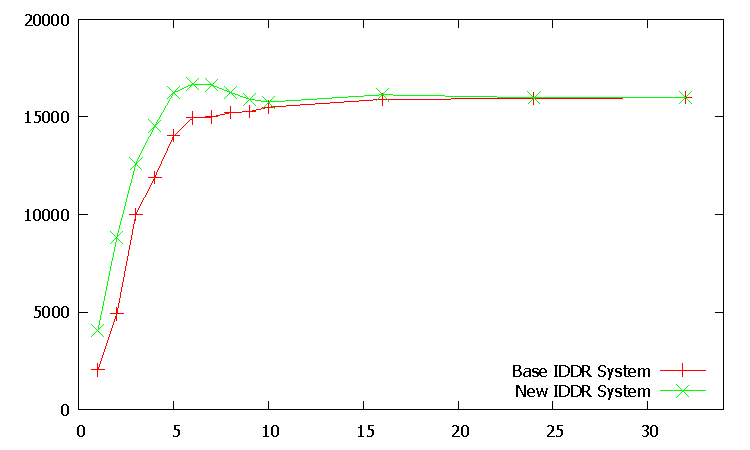
\includegraphics[scale=.7]{rndwr-loopdisk}
  \caption{Random writes}
  \label{subfig:rndwr-loopdisk}
  \end{subfigure}\\
  \begin{subfigure}[b]{0.3\textwidth}
  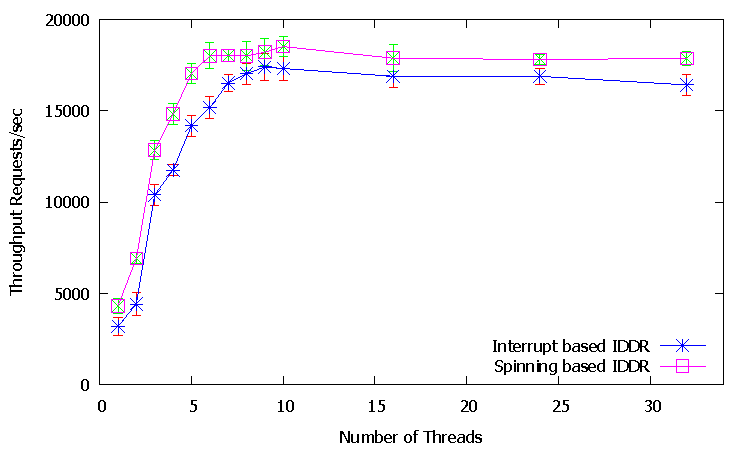
\includegraphics[scale=.7]{rndrw-loopdisk}
  \caption{Random reads writes}
  \label{subfig:rndrw-loopdisk}
  \end{subfigure}
\caption{Random reads and writes on a Loop device}\label{fig:rndloopdisk}
\end{figure}

\begin{figure}[!ht]
%\centering
  \begin{subfigure}[b]{0.2\textwidth}
  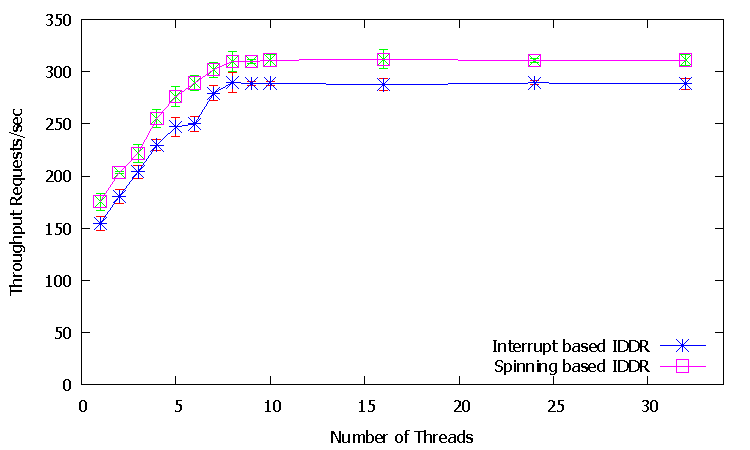
\includegraphics[scale=.7]{rndrd-harddisk}
  \caption{Random reads}
  \label{subfig:rndrd-harddisk}
  \end{subfigure}
  \hspace{50mm}
  \begin{subfigure}[b]{0.2\textwidth}
  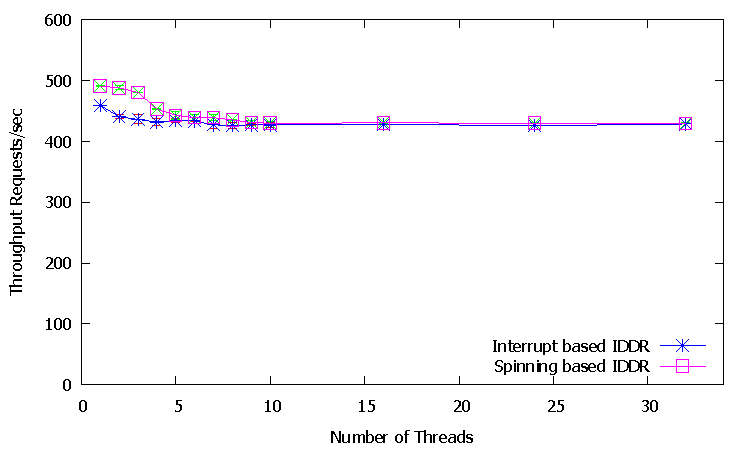
\includegraphics[scale=.7]{rndwr-harddisk}
  \caption{Random writes}
  \label{subfig:rndwr-harddisk}
  \end{subfigure}\\
  \begin{subfigure}[b]{0.3\textwidth}
  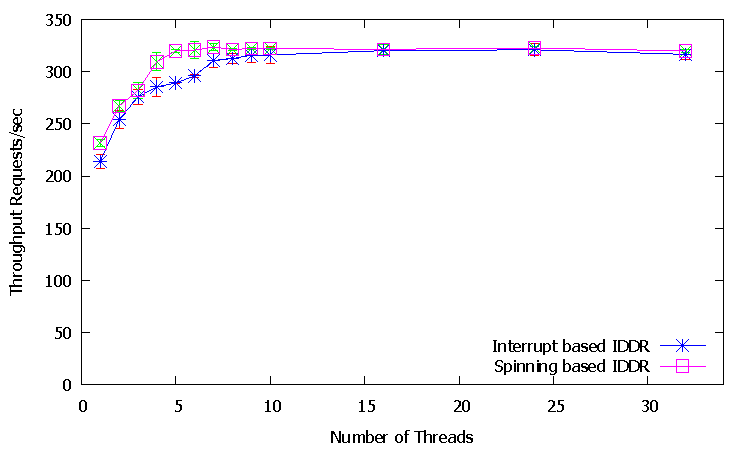
\includegraphics[scale=.7]{rndrw-harddisk}
  \caption{Random reads writes}
  \label{subfig:rndrw-harddisk}
  \end{subfigure}
\caption{Random reads and writes on a SATA disk}\label{fig:rndharddisk}
\end{figure}


\paragraph{Observation :}
The performance analysis of the interrupt based and spinning IDDR system shows that initially the throughput of the system increases and then it remains constant. We measure the throughput of the system with varying number of SysBench threads. 

In both the systems, when the number of SysBench threads is low, the rate at which data is read and written is low and when number of SysBench threads is high, the rate at which data is read and written is high. Low data workload results in low throughput and high data workload results in high data throughput. Once maximum throughput is achieved, it remains constant.

In interrupt based IDDR system, virtual interrupt is send between application domain and driver domain for read and write requests and in spinning based IDDR system, both the domains spin for the request and responses. Our optimization technique reduces the frequency of the virtual interrupt being sent between domains. Hence the improvement in performance depends upon number of virtual interrupts avoided. In the interrupt based IDDR system, when data workload is low, requests are generated with larger gaps of interval. Hence less number of requests are batched together, which results in more virtual interrupts. However, high workload observes more requests being batched together. Since spinning based IDDR system avoids more portion of virtual interrupts when workload is low, we observe a more performance gain when data workload is low. 

\subsubsection*{CPU utilization}

In spinning based IDDR system the frontend and backend driver spin for the request and responses and uses the CPU cycles. Hence we see a trade-off between high CPU utilization and high throughput. 

In this section we compare the CPU utilization of interrupt based and spinning based IDDR system.

Figure~\ref{fig:cpuramdisk}, Figure~\ref{fig:cpuloopdisk} and Figure~\ref{fig:cpuharddisk} compares the CPU performance of both the systems with ramdisk, loop device and SATA disk as a physical device. 

\paragraph{Observation: }
Since in IDDR system, read response thread and read request thread spin continuously both threads consume 2 cores of the system all the time. In below graphical presentation, 100\% CPU utilization denotes full utilization of 1 CPU. It can be seen that CPU utilization of spinning based system is near 200\% i.e. 2 cores. 

\begin{figure}[!ht]
%\centering
  \begin{subfigure}[b]{0.2\textwidth}
  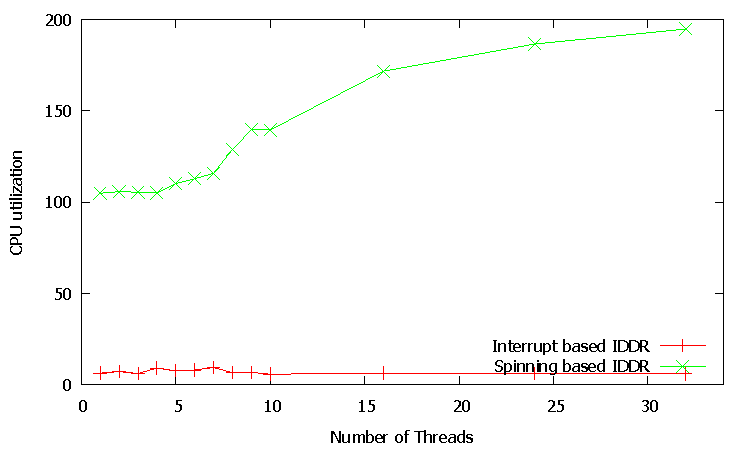
\includegraphics[scale=.7]{cpu-rndrd-ramdisk}
  \caption{Random reads}
  \label{subfig:cpu-rndrd-ramdisk}
  \end{subfigure}
  \hspace{50mm}
  \begin{subfigure}[b]{0.2\textwidth}
  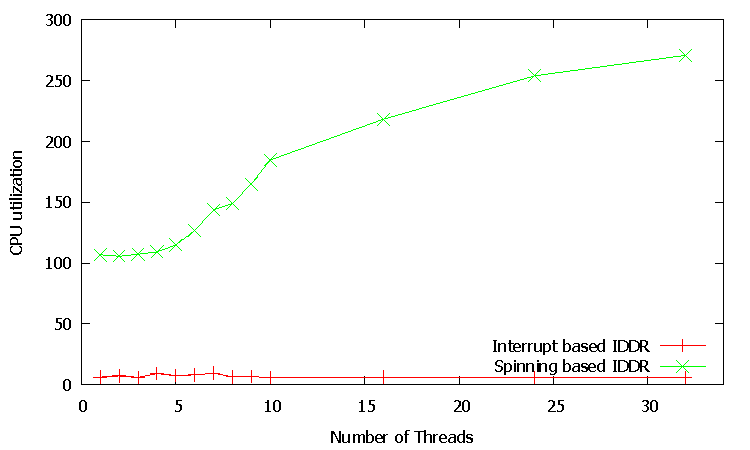
\includegraphics[scale=.7]{cpu-rndrw-ramdisk}
  \caption{Random writes}
  \label{subfig:cpu-rndrw-ramdisk}
  \end{subfigure}\\
  \begin{subfigure}[b]{0.3\textwidth}
  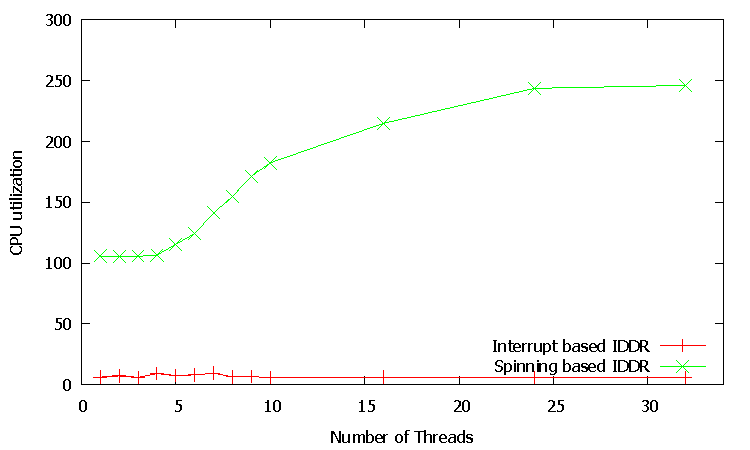
\includegraphics[scale=.7]{cpu-rndwr-ramdisk}
  \caption{Random reads writes}
  \label{subfig:cpu-rndwr-ramdisk}
  \end{subfigure}
\caption{Comparison of CPU utilization - ram disk}\label{fig:cpuramdisk}
\end{figure}

\begin{figure}[!ht]
  \begin{subfigure}[b]{0.2\textwidth}
  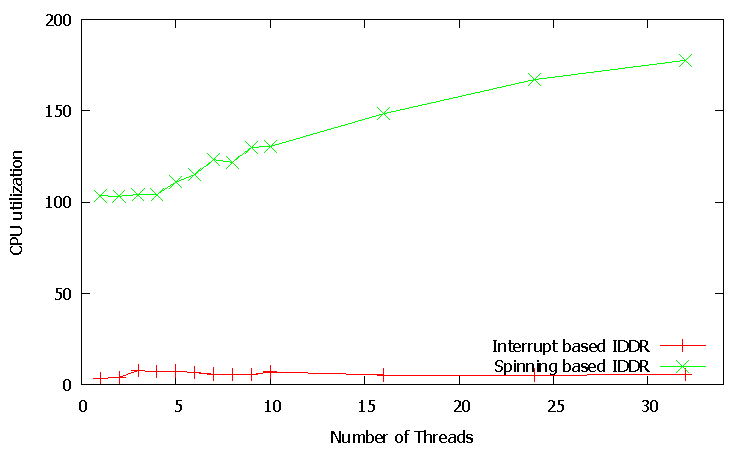
\includegraphics[scale=.7]{cpu-rndrd-loopdisk}
  \caption{Random reads}
  \label{subfig:cpu-rndrd-loopdisk}
  \end{subfigure}
  \hspace{50mm}
  \begin{subfigure}[b]{0.2\textwidth}
  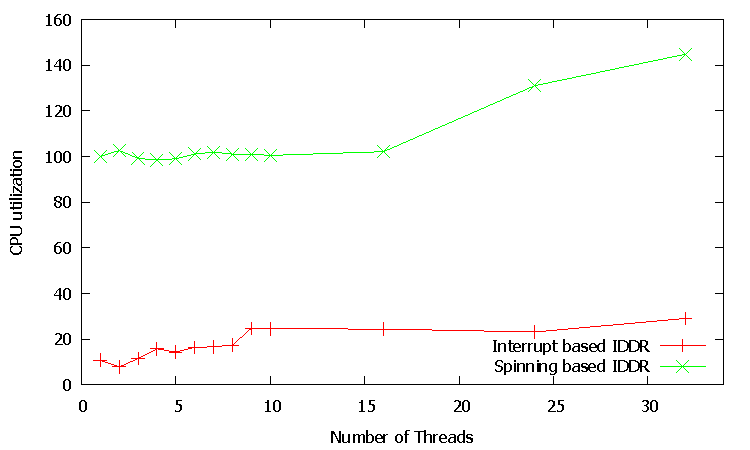
\includegraphics[scale=.7]{cpu-rndrw-loopdisk}
  \caption{Random writes}
  \label{subfig:cpu-rndrw-loopdisk}
  \end{subfigure}\\
  \begin{subfigure}[b]{0.3\textwidth}
  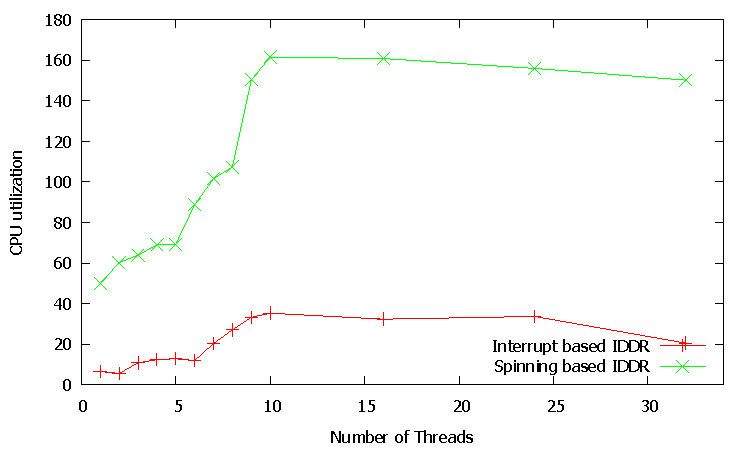
\includegraphics[scale=.7]{cpu-rndwr-loopdisk}
  \caption{Random reads writes}
  \label{subfig:cpu-rndwr-loopdisk}
  \end{subfigure}
\caption{Comparison of CPU utilization - loop device}\label{fig:cpuloopdisk}
\end{figure}

\begin{figure}[!ht]
%\centering
  \begin{subfigure}[b]{0.2\textwidth}
  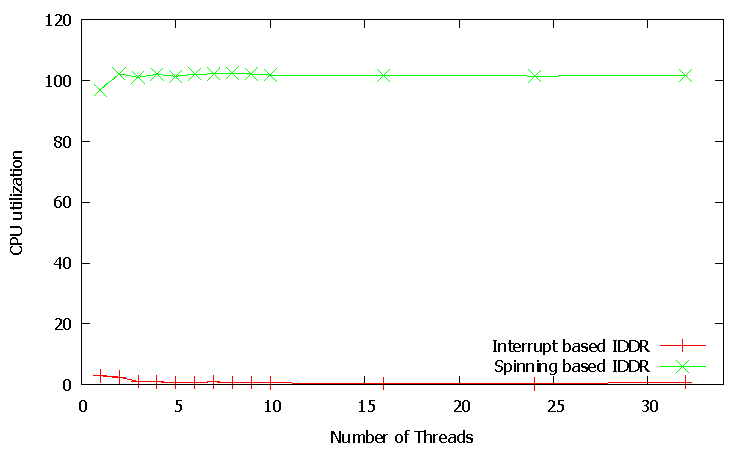
\includegraphics[scale=.7]{cpu-rndrd-harddisk}
  \caption{Random reads}
  \label{subfig:rndrd-harddisk}
  \end{subfigure}
  \hspace{50mm}
  \begin{subfigure}[b]{0.2\textwidth}
  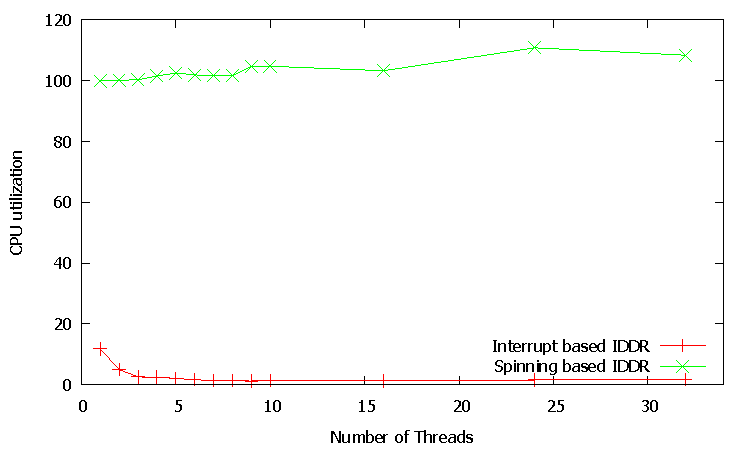
\includegraphics[scale=.7]{cpu-rndwr-harddisk}
  \caption{Random writes}
  \label{subfig:rndwr-harddisk}
  \end{subfigure}\\
  \begin{subfigure}[b]{0.3\textwidth}
  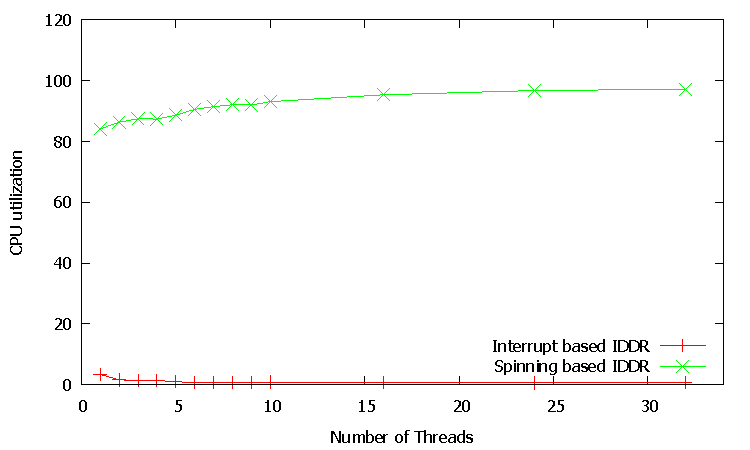
\includegraphics[scale=.7]{cpu-rndrw-harddisk}
  \caption{Random reads writes}
  \label{subfig:rndrw-harddisk}
  \end{subfigure}
\caption{Comparison of CPU utilization - SATA disk}\label{fig:cpuharddisk}
\end{figure}



\ifbool{toShowBibliography}{\bibliography{references}}{}

\chapter{Related Work}
\markright{Sushrut Shirole \hfill Chapter 5. Related Work \hfill}

This chapter briefly discusses work closely related to the IDDR System. Our work is divided into two parts: 
\begin{enumerate}
\item Implementation of the isolated driver domain which improves the reliability of the system 
\item Performance improvement of inter-domain communication in the isolated driver domain 
\end{enumerate}
This chapter is divided into two sections. Section~\ref{sec:robustness} discusses work on improving the reliability of a system and Section~\ref{sec:interdomain} discusses work which concentrates on improving inter-domain communication.
\\[3mm]

\section{Reliability of the System}
\label{sec:robustness}
The goal of the baseline implementation of the IDDR system is to increase the reliability of an operating system. In this section we describe research in the operating systems area which focuses on increasing the reliability of a system.

\subsection{Driver Protection Approaches}
A faulty device driver causes a significant number of failures in the Linux kernel~\cite{tanenbaum2006can, coveritykernel}. In the past, research in areas, such as hardware based driver isolation, language based driver isolation and user level device drivers, has contributed towards isolating device drivers, hence increasing the reliability of a system.
\\[3mm]
Numerous implementations run device drivers in the user mode. Even though user mode device drivers allow user level programming and a good fault isolation between components, they suffer from poor performance~\cite{armand1991give} and also require re-writing of the existing device drivers. The user mode device drivers also lack compatibility~\cite{Leslie+:jcst2005}. Microdrivers~\cite{Ganapathy:2008:DIM:1346281.1346303} extend the user mode device driver research and split a device driver into two parts. In Microdrivers, performance critical operations of the device driver run in the kernel and the rest of the driver code runs in a user mode process. Microdrivers deliver good performance and compatibility.
\\[3mm]
Apart from user mode device driver, some approaches use hardware based driver isolation to achieve the isolation between components. Nooks is one example of such approaches. Nooks~\cite{swift2005improving} maintains the monolithic kernel structure, and focuses on making device drivers less vulnerable. It creates a lightweight protection domain around each device driver. The domain is created by wrapping a layer of protective software around a device driver. The wrapper layer monitors all interactions between the driver and the kernel, and protects the kernel from a faulty device driver. Nooks requires device drivers to be modified as their interaction with the kernel changes. 
\\[3mm]
SUD~\cite{Boyd-Wickizer+:atc2010} runs unmodified Linux device drivers in the user space. It uses the emulated IOMMU hardware to run a device driver in the user space. Running device drivers in a user space safely isolates a system from a malicious device driver. 
\\[3mm]
Dune~\cite{Belay+:osdi12} is a system that provides an application direct and safe access to the hardware features, such as page tables, tagged TLBs and ring protection. It uses virtualized hardware to isolate applications from each other. Dune delivers hardware interrupts directly to applications in order to improve the signal delivery performance. However, Dune does not isolate device drivers from each other.

\subsubsection*{Virtualization Based Approaches}
The IDDR system isolates a device driver from a Linux kernel using Xen VMM. Research work, which uses virtualization techniques to isolate the kernel components is related more closely to our work.
\\[3mm]
Xen isolated driver domain~\cite{Fraser04safehardware} is a device driver isolation architecture presented by Xen. The isolated device driver allows unmodified device drivers to be run in a separate domain and shared across operating system instances. Isolated driver domain protects individual operating systems, from driver failure. The base IDDR system is the re-implementation of Xen isolated driver domain. 
\\[3mm]
LeVesseur et. al.~\cite{LeVasseur04UnmodifiedDriverReuse} presents a virtualization based system to reuse unmodified device drivers. It also improves system reliability. In this approach, an unmodified device driver is run with a kernel in a separate virtual machine. The main goal of this system is to reuse the device driver across different operating systems. However, the system isolates faults caused by a device driver by running a device driver in separate virtual machine.
\\[3mm]
VirtuOS~\cite{Nikolaev:2013:VOS:2517349.2522719} is a library level solution that allows processes to directly communicate with a domain. VirtuOS exploits
virtualization to isolate the components of existing OS kernels in separate virtual machines. These virtual machines directly serve system calls from
user processes.

\subsection{Other Approaches}
\subsubsection*{Kernel Based Approach}
In this approach, systems provide a better fault containment by disintegrating the kernel functionality as system components. Microkernels are examples of such approaches. They provide fault containment by providing an isolation between the system components. In the microkernels such as Mach~\cite{Accetta+:usenix86} and L4~\cite{Liedtke+:sosp95}, only essential functionalities like memory management, interprocess communication, scheduling and low level device drivers are implemented in the kernel. Remaining system components, like file system and process management are implemented as user processes.
\\[3mm]
Some of the recent work also uses the similarity in the abstraction provided by the hypervisor and microkernel. Microvisor~\cite{Heiser+:acm10} is a kernel that satisfies the combined objectives of microkernels and hypervisors, and provides an abstraction of a virtual machine, where a guest OS schedules activities on one or more VCPUs.

\section{Inter-domain Communication}
\label{sec:interdomain}
In the past numerous work on inter domain communication mechanisms was presented. In Xen VMM, a domain communicates with the privileged domain through the split device driver mechanism~\cite{Fraser04safehardware}. In a way, the split device driver mechanism is a restricted inter domain communication path. The Xen split driver faces the performance issues becuase of the overhead of numerous context switches in form of event channel interrupts. It also incurs an overhead due to an extra data copy and page flipping~\cite{Zhang:2007:XHI:1516124.1516138}. 
\\[3mm]
In order to overcome the page flipping performance overhead, Xen hypervisor also provides a UNIX domain socket like interface called XenSocket~\cite{Zhang:2007:XHI:1516124.1516138}. XenSocket provides a high throughput inter-domain communication. It replaces the page flipping design of the split driver. However, XenSocket needs an existing socket interface APIs to be changed. 
\\[3mm]
Fido~\cite{Burtsev:2009:FFI:1855807.1855832} is a shared memory based inter domain communication mechanism. Fido implements the fast inter-domain communication mechanism by reducing data copies in the Xen hypervisor. In contrast, the IDDR system improves the inter domain communication mechanism of Split device drivers by avoiding the context switches. Also, Fido removes overhead with zero copy by sacrificing the security and protections guarantees.
\\[3mm]

\ifbool{toShowBibliography}{\bibliography{references}}{}


\chapter{Conclusion}
\markright{Sushrut Shirole \hfill Chapter 7. Conclusion\hfill}


In this thesis we presented the Isolated Device Driver (IDDR) system. The IDDR system is an operating system which provides isolation between a device driver and the Linux kernel components by running the device driver in the driver domain. The IDDR system is a re-implementation of Xen's isolated driver domain.

Isolated driver domains use Xen's split device driver mechanism. Originally split device drivers exploit an interrupt based approach to interdomain communication. We replaced the interrupt based approach with a spinning based approach. This spinning based approach has the potential to reduce interdomain communication overhead including the number of context switch. IDDR system trades CPU cycles for better performance.

The IDDR system will be advantageous if used with I/O intensive applications. I/O intensive system can afford to utilize the idle CPU cycles for the benefit of the performance. 

\section{Future Work}
\paragraph{Adaptive spinning : }
In current implementation the read request thread and read response thread spins for a constant amount of time. It will be interesting to see the impact on performance if adaptive spinning is used.

%%%%%%%%%%%%%%%%
% Do tables like this:

%  \begin{table}
%  \caption{The Graduate School wants captions above the tables.}
% \begin{center}
%  \begin{tabular}{ccc}
%  x & 1 & 2 \\ \hline
%  1 & 1 & 2 \\
%  2 & 2 & 4 \\ \hline
%  \end{tabular}
% \end{center}
%  \end{table}

%%%%%%%%%%%%%%%%%
% all sections and sub-sections

%\part
%\chapter (report style only)
%\section
%\subsection
%\subsubsection
%\paragraph
%\subparagraph
%\subsubparagraph (milstd and book-form styles only)
%\subsubsubparagraph (milstd and book-form styles only)

%%%%%%%%%%%%%%%%%%%%%%%%%%%%%%%%

\nocite{*}
\bibliographystyle{plain}
\bibliography{references}
\end{document}